%Version 3.1 December 2024
% See section 11 of the User Manual for version history
%
%%%%%%%%%%%%%%%%%%%%%%%%%%%%%%%%%%%%%%%%%%%%%%%%%%%%%%%%%%%%%%%%%%%%%%
%%                                                                 %%
%% Please do not use \input{...} to include other tex files.       %%
%% Submit your LaTeX manuscript as one .tex document.              %%
%%                                                                 %%
%% All additional figures and files should be attached             %%
%% separately and not embedded in the \TeX\ document itself.       %%
%%                                                                 %%
%%%%%%%%%%%%%%%%%%%%%%%%%%%%%%%%%%%%%%%%%%%%%%%%%%%%%%%%%%%%%%%%%%%%%

%%\documentclass[referee,sn-basic]{sn-jnl}% referee option is meant for double line spacing

%%=======================================================%%
%% to print line numbers in the margin use lineno option %%
%%=======================================================%%

%%\documentclass[lineno,pdflatex,sn-basic]{sn-jnl}% Basic Springer Nature Reference Style/Chemistry Reference Style

%%=========================================================================================%%
%% the documentclass is set to pdflatex as default. You can delete it if not appropriate.  %%
%%=========================================================================================%%

%%\documentclass[sn-basic]{sn-jnl}% Basic Springer Nature Reference Style/Chemistry Reference Style

%%Note: the following reference styles support Namedate and Numbered referencing. By default the style follows the most common style. To switch between the options you can add or remove Numbered in the optional parenthesis. 
%%The option is available for: sn-basic.bst, sn-chicago.bst%  
 
%%\documentclass[pdflatex,sn-nature]{sn-jnl}% Style for submissions to Nature Portfolio journals
%%\documentclass[pdflatex,sn-basic]{sn-jnl}% Basic Springer Nature Reference Style/Chemistry Reference Style
\documentclass[pdflatex,sn-mathphys-num]{sn-jnl}% Math and Physical Sciences Numbered Reference Style
%%\documentclass[pdflatex,sn-mathphys-ay]{sn-jnl}% Math and Physical Sciences Author Year Reference Style
%%\documentclass[pdflatex,sn-aps]{sn-jnl}% American Physical Society (APS) Reference Style
%%\documentclass[pdflatex,sn-vancouver-num]{sn-jnl}% Vancouver Numbered Reference Style
%%\documentclass[pdflatex,sn-vancouver-ay]{sn-jnl}% Vancouver Author Year Reference Style
%%\documentclass[pdflatex,sn-apa]{sn-jnl}% APA Reference Style
%%\documentclass[pdflatex,sn-chicago]{sn-jnl}% Chicago-based Humanities Reference Style

%%%% Standard Packages
%%<additional latex packages if required can be included here>

\usepackage{graphicx}%
\usepackage{multirow}%
\usepackage{amsmath,amssymb,amsfonts}%
\usepackage{amsthm}%
\usepackage{mathrsfs}%
\usepackage[title]{appendix}%
\usepackage{xcolor}%
\usepackage{textcomp}%
\usepackage{manyfoot}%
\usepackage{booktabs}%
\usepackage{algorithm}%
\usepackage{algorithmicx}%
\usepackage{algpseudocode}%
\usepackage{listings}%
\usepackage{rotating}%
\usepackage{subfigure}%
\usepackage{color}%
\usepackage{float}%
\usepackage{microtype}%
\usepackage{url}%
\usepackage{hyperref}%
\usepackage{adjustbox}%
\usepackage{placeins}%
\usepackage{longtable}%
\usepackage{pdflscape}%
\usepackage{pgfplots}%
\pgfplotsset{compat=1.18}
%%%%

%%%%%=============================================================================%%%%
%%%%  Remarks: This template is provided to aid authors with the preparation
%%%%  of original research articles intended for submission to journals published 
%%%%  by Springer Nature. The guidance has been prepared in partnership with 
%%%%  production teams to conform to Springer Nature technical requirements. 
%%%%  Editorial and presentation requirements differ among journal portfolios and 
%%%%  research disciplines. You may find sections in this template are irrelevant 
%%%%  to your work and are empowered to omit any such section if allowed by the 
%%%%  journal you intend to submit to. The submission guidelines and policies 
%%%%  of the journal take precedence. A detailed User Manual is available in the 
%%%%  template package for technical guidance.
%%%%%=============================================================================%%%%

%% as per the requirement new theorem styles can be included as shown below
\theoremstyle{thmstyleone}%
\newtheorem{theorem}{Theorem}%  meant for continuous numbers
%%\newtheorem{theorem}{Theorem}[section]% meant for sectionwise numbers
%% optional argument [theorem] produces theorem numbering sequence instead of independent numbers for Proposition
\newtheorem{proposition}[theorem]{Proposition}% 
%%\newtheorem{proposition}{Proposition}% to get separate numbers for theorem and proposition etc.

\theoremstyle{thmstyletwo}%
\newtheorem{example}{Example}%
\newtheorem{remark}{Remark}%

\theoremstyle{thmstylethree}%
\newtheorem{definition}{Definition}%

\raggedbottom

%%\unnumbered% uncomment this for unnumbered level heads

\begin{document}

\title[Subchat Trees]{Subchat Trees: A Scalable Hierarchical Architecture for Multi-Threaded Dialogue and Context Isolation in LLMs}

\author*[1]{\fnm{Mehedi Hasan} \sur{Moon}}\email{the.mehedi.hasan.moon@gmail.com}

\author[1]{\fnm{Kabbo Sarker} \sur{Surjo}}\email{kabbosarker29@gmail.com}

\author[1]{\fnm{Md.} \sur{Akhtaruzzaman}}\email{akhter900@cse.mist.ac.bd}

\affil*[1]{\orgdiv{Department of Computer Science and Engineering}, \orgname{Military Institute of Science and Technology (MIST)}, \orgaddress{\city{Dhaka}, \country{Bangladesh}}}

%%==================================%%
%% ABSTRACT                        %%
%%==================================%%


% \abstract{Current LLM chat interfaces are still organized mainly as linear transcripts: every topic, correction, side question, and follow-up is appended to the same chronological history. This design works for short single-topic exchanges, but it becomes fragile in realistic long conversations where users switch between tasks, return to earlier topics, or open nested follow-ups. Unrelated context can leak across topics, older details can be evicted or buried, and increasing the model's context length alone does not decide which part of the conversation should be active. We introduce \textit{Subchat Trees}, a user-facing nested branching architecture for conversation management. Instead of treating the chat as one flat buffer, Subchat Trees represents dialogue as a tree of parent and child subchats, where each node maintains its own local buffer, rolling summary, and vector-indexed long-term memory. A user can create a focused subchat from a selected parent fragment, continue a detailed side discussion in that branch, and later return to the parent without contaminating sibling or ancestor contexts. This external conversation structure is model-agnostic and can improve LLM behavior without fine-tuning, because the model receives a cleaner branch-local context at inference time. We evaluate the approach on a 309-turn Variable-Block Randomized Interleaving (VBRI) benchmark derived from five LMSYS-Chat-1M conversations, covering 59 topic labels and 43 topic-recall probes. Across Qwen2.5 7B, 14B, and 32B AWQ models and buffer sizes $C \in \{5,10,20,40\}$, Subchat Trees improves context-isolation F1 over the linear baseline in every model-buffer setting. The best absolute result occurs with the 32B model at $C=20$, where F1 improves from 69.6\% to 85.2\% and topic pollution falls from 32.7\% to 16.5\%. The 14B model provides the strongest practical tradeoff, reaching 83.4\% F1 at $C=10$ and 83.1\% at $C=20$. Recall probes also show stronger topic retention: average ROUGE-1 improves over baseline in all tested settings, including 0.2476 to 0.4187 for 14B at $C=20$ and 0.3338 to 0.4283 for 32B at $C=20$. Although raw input tokens sometimes increase because cleaner context elicits fuller answers, tokens per correct answer decreases across all tested configurations. These results suggest that complex conversations need explicit external structure, not only longer context windows, and that nested branching is a practical interface-level method for improving long-running LLM reliability.}





%HUMANIZE
\abstract{
Current LLM chat interfaces use linear transcripts to communicate with the user. In linear conversation every topic, sub-topic and even follow-up is appended to the same chronological history. This design is useful for short single-topic conversations but it becomes fragile in realistic long-term conversations. Where users switch between task/topic, return or mention earlier topic or ask nested follow-ups. Human conversations naturally follow a hierarchical structure but modern day AI interface lack conversational flow control in their interfaces. As a result, Unrelated context can leak across topics and older context can be evicted or buried. Current studies try to address this problem by increasing context length and models complexity. But Human conversation lacks its natural flow in chat interface. We see it as a design problem and propose Subchat Trees, a user-facing nested branching architecture for conversation management. Instead of treating the chat as one flat linear conversation, SubchatTree represents dialogue as a tree of parent and child subchats, where each node maintains its own local buffer, rolling summary and  a shared vector-indexed long-term memory. A user can create a focused subchat from a selected parent excerpt, continue a side discussion in that branch and later return to parent without contaminating sibling or ancestor contexts. This external architecture is model-agnostic and can imporve LLM performance without fine-tuning, as the model receives a cleaner branch-local context at inference time. The approach was evaluated on a controlled 353 turn Variable-Block Randomized Interleaving (VBRI) stress-test benchmark derived from five LMSYS-Chat-1M conversations, covering 59 topic labels and 43 topic-recall probes. Across Qwen2.5 7B, 14B and 32B models and buffer sizes $C \in \{5,10,20,40\}$. SubchatTrees improves context-isolation F1 over the linear baseline in every model-buffer setting. The best performing model was Qween32B at $C=20$, with an F1 score of 85.2\% and pollution rate was 16.2\%. Recall probes also show stronger topic retention. Average ROUGE-1 improves over baseline in all tested settings, including 0.2476 to 0.4187 for 14B at $C=20$ and 0.3338 to 0.4283 for 32B at $C=20$. A reduction in input token per correct answer is also observed across all tested configurations. The results suggest that complex conversations need explicit external structure, not only longer context windows.
}




\keywords{Large Language Models, Conversational AI, Hierarchical Dialogue, Context Isolation, Retrieval-Augmented Generation, Multi-threaded Conversations}

\maketitle

%%==================================%%
%% SECTION 1: INTRODUCTION         %%
%%==================================%%

\section{Introduction}\label{sec1}

% Large language models now serve as the backbone of chat systems used for programming assistance, education, planning, research, and open-domain dialogue. Despite these gains, failures remain common in long, multi-topic conversations: earlier constraints are forgotten, separate tasks become mixed, and outdated turns keep influencing later responses. These pathologies persist because most chat interfaces still organize every exchange as a single chronological transcript, even when the underlying interaction contains multiple partially overlapping threads. As sessions grow, this flat structure increases context pollution and makes it harder for the model to recover the right information at the right time~\cite{liu2023lostinthemiddle,laban2024limt}.





% HUMANIZE

Large language models now serve as the backbone of chat systems used for programming assistance, education, planning, research and open-domain dialogue. Despite this advancement, failures remain common in long, multi-topic conversations. Earlier constraints are forgotten, separate task become mixed and outdated turns keep influencing later responses. This problem persists because most chat interface still organize every turn into a single chronological transcript, even when the underlying interaction contains multiple partially overlapping threads. As session grows, this chronological structure increase context pollution and makes it harder for the model to recover right information at the right time ~\cite{liu2023lostinthemiddle,laban2024limt}.








% At the same time, several research directions suggest that explicit structure can improve language-model behaviour. Chain-of-Thought, Self-Consistency, Tree-of-Thought, and Graph-of-Thought show that structured intermediate reasoning improves problem solving on complex tasks~\cite{wei2022cot,wang2023selfconsistency,yao2023tot,besta2023got}. Conversation disentanglement studies show that mixed message streams naturally contain distinct threads, but recovering those threads after the fact is difficult and error-prone~\cite{elsner2008talking,jiang2018disentangle,kummerfeld2019disentanglement}. Hierarchical dialogue models, memory systems, retrieval augmentation, and role-based interaction frameworks likewise add structure at different levels of the stack~\cite{serban2016hred,packer2023memgpt,wu2024stateful,lewis2020rag,li2023camel}.


Recent studies suggest that explicit structure can improve language-model performance. Studies including  Chain-of-Thought, Self-Consistency, Tree-of-
Thought and Graph-of-Thought show that structured intermediate reasoning can improve LLM problem- solving ability on complex tasks. Conversation disentangle studies show that mixed message streams naturally contain distinct threads, but separating this thread after the fact is difficult and error-prone~\cite{elsner2008talking,jiang2018disentangle,kummerfeld2019disentanglement}. Other studies such as Hierarchical dialogue models, memory systems, retrieval augmentation and role-based interaction frameworks also introduce structure into how conversations are represented, stored, retrieved and managed ~\cite{serban2016hred,packer2023memgpt,wu2024stateful,lewis2020rag,li2023camel}.











% More recent work treats multi-turn interaction as a distinct capability regime rather than a simple repetition of single-turn prompting. Long-context studies show that relevant evidence becomes harder to use when it is buried in the middle of an input sequence~\cite{liu2023lostinthemiddle}. Dialogue-focused benchmarks and memory studies report similar degradation across long-running interactions, including failures in factual consistency, event recall, and persona tracking~\cite{laban2024limt,maharana2024locomo,xu2022goldfish,xu2022longpersona}. Prompt compression can reduce token cost and improve information density, but it still operates over a fundamentally linear interaction record~\cite{jiang2024longllmlingua}.






More recent work shows that multi-turn interaction is not simply repeated single term prompting. It is treated as a separate challenge that requires models to track users context, state and intent over time. This can be observed for multi-agents systems as well. Long-context studies show that relevent evidence becomes harder to use when it is buried in the middle of a input sequence~\cite{liu2023lostinthemiddle}. Dialogue-focused studies also observed similar degradation pattern over long-running interaction such as, failures in factual consistency, event recall and context tracking~\cite{laban2024limt,maharana2024locomo,xu2022goldfish,xu2022longpersona}. Context compression can reduce token cost and imporve information density, but again this can compress multiple distinct threads into a single one~\cite{jiang2024longllmlingua}.










Consider a user who starts with Python debugging, shifts to python snakes for a biology question, opens a side discussion about Linux audio, and later returns to the original code. In a linear transcript, the latest query is interpreted against an interleaved history where keywords, pronouns, and instructions now refer to multiple competing contexts. The result can be semantic drift, role confusion, privacy leakage between topics and unnecessary token growth from carrying a broad history that no longer belongs to the current task.




% The central issue, is not only how to store more context, but how to organize context so that unrelated conversational threads stop competing with one another. \textit{Subchat Trees} addresses this problem at the interaction layer. Rather than asking the model to untangle a mixed transcript internally, the interface preserves topic structure explicitly through branch creation, local buffers, rolling summaries, and branch-scoped retrieval. The goal is to keep active context focused while still allowing long-term information to remain accessible.



The central issue, is not only how to store more context, but how to organize them so that unrelated conversational threads stop competing with one another. \textit{SubchatTrees} address this problem at the interaction layer. Rather than asking the model to untangle a mixed transcript, the interface preserves topic structure explicitly through branch creation, local buffer, rolling summaries and branch-scoped retrieval. The goal is to keep active context focused, while still allowing long-term information to remain accessible.









\subsection{Overview of Subchat Trees}\label{subsec:approach}

\textbf{SubchatTrees} organizes a session as a tree of related dialogue nodes rather than a single linear transcript. The design goal is to keep each active branch semantically focused while still allowing information to grow and persist through summarization and retrieval. The architecture centers on four design elements:




\begin{itemize}
    \item Each conversation node maintains isolated context through local circular buffers ($C$ messages) and vector-indexed long-term memory.
    \item Users create focused ``subchats'' by selecting specific text fragments from parent conversations.
    \item Follow-up prompts inject selected context as system messages, guiding the LLM's attention.
    \item Parallel reasoning threads coexist without interference, and rolling summarization preserves semantic continuity beyond the buffer horizon.
\end{itemize}

\subsection{Objectives}\label{subsec:objectives}

\begin{enumerate}
    % \item To reduce context pollution in long, multi-topic conversations by separating unrelated threads into branch-local dialogue contexts.
    \item To minimize context pollution in long, multi-topic conversations by separating unrelated threads thorugh chat interface.



    \item To enable isolated and focused sub-conversations (subchats) where users can pursue side discussions without contaminating parent or sibling contexts.
    \item To implement scalable memory management through a tree-structured conversation architecture that combines local buffers, rolling summaries and retrieval-based long-term memory.
    
    % \item To reduce latency while maintaining conversation quality by providing the model with more relevant, branch-specific context at inference time.
    
    \item To reduce latency and token cost while maintaining conversation quality by providing the model with more relevant context at inference time.

\end{enumerate}

Section~\ref{sec2} reviews prior work on dialogue modelling, structured reasoning, memory, retrieval, disentanglement, and multi-turn interaction. Section~\ref{sec3} describes the system architecture and evaluation methodology. Section~\ref{sec4} reports the experimental results, and Sections~\ref{sec5} and~\ref{sec6} discuss implications and conclusions.



%%==================================%%
%% SECTION 2: RELATED WORK         %%
%%==================================%%

\section{Related Work}\label{sec2}

% Modern work on multi-turn LLM systems builds on a longer line of sequence modeling research. Early encoder-decoder models showed that end-to-end neural systems could map one sequence to another within a unified framework~\cite{sutskever2014seq2seq}. Attention mechanisms then reduced the bottleneck of fixed-length sequence representations~\cite{bahdanau2014attention}, and the Transformer made attention the dominant architecture for large-scale language modeling and generation~\cite{vaswani2017attention}. With scale, autoregressive models began to exhibit broad in-context task adaptation, most visibly in GPT-3's few-shot results~\cite{brown2020gpt3}. Instruction tuning and alignment work then pushed these systems closer to practical task-following assistants by improving zero-shot generalization and adherence to user intent~\cite{wei2022flan,ouyang2022instructgpt}. Against that background, current research on long-context and multi-topic dialogue focuses less on basic language generation and more on how context should be organized, retrieved, and controlled during interaction.





Modern work on multi-turn LLM systems builds on a longer line of sequence modeling  and neural dialogue research. Early encoder-decoder models showed that neural network could learn to map an input sequence to an output sequence~\cite{sutskever2014seq2seq}. The transformer based attention mechanism  reduced the bottleneck of fixed-length sequence representations~\cite{bahdanau2014attention}, becoming the foundation of modern large-language models~\cite{vaswani2017attention}. Later, autoregressive models began to exhibit broad in-context task adaptation, like GPT-3's few-shot results ~\cite{brown2020gpt3}. Futher, Instruction tuning and alignment work made this model practical task-following assistants by improving zero-shot generalization and their ability to follow user intent~\cite{wei2022flan,ouyang2022instructgpt}. Against that background, current studies are more focused on how context should be organized, retrived and controlled during interaction.



\subsection{Background: End-to-End Dialogue Modelling}\label{subsec:dialogue_background}

Before the current wave of instruction-following LLM systems, dialogue modelling was often approached through end-to-end generative architectures trained on conversational corpora. Early studies like, Hierarchical recurrent encoder-decoder models (HRED) introduced a two-level structure in which token sequences formed utterances and utterances formed conversations~\cite{serban2016hred}. This work  established an early argument that dialogues can be benefitted from explicit hierarchical organization rather than flat sequence processing alone.

Though the hierarchy remains internal to the model rather than exposed in the interaction design. But it proves that structure can improved model's performance.

\subsection{Structured Reasoning and Branching Search}\label{subsec:reasoning}

Chain-of-Thought prompting shows that exposing intermediate reasoning steps can significantly improve models performance on complex reasoning tasks that require multi step inference~\cite{wei2022cot}. Self-Consistency extends this idea by sampling multiple reasoning paths and aggregating them rather than trusting a single chain~\cite{wang2023selfconsistency}. Tree-of-Thought and Graph-of-Thought push the same idea further by representing reasoning as a branching or graph-structured search process rather than a single linear derivation~\cite{yao2023tot,besta2023got}.






% Taken together, these methods support a broader conclusion: structured representations can improve robustness, interpretability, and search efficiency. Their scope, however, is usually limited to single tasks or single prompts. They do not specify how multi-topic conversational history should be segmented over time. Subchat Trees adopts the same high-level intuition about branching and decomposition, but applies it to persistent interaction structure rather than only to reasoning traces.



Taken together these studies suggest a broader conclusion. Structured representation and proper context engineering can improve models robustness, interpretability and search efficiency. Though their scope is limited to single tasks or single prompts, but subchat trees adopts the same high-level intuition about branching and decomposition. Though it is  applied to persistent interaction structure rather than only to reasoning traces.








\subsection{Context, Memory, and Retrieval}\label{subsec:memory_related}

The limitations of long multi-turn conversational history are now well establish. Phenomenon such as ``Lost in the middle'' shows that language models exhibit strong position bias. Often struggle to utilize evidence placed in the middle of a conversation or prompt~\cite{liu2023lostinthemiddle}. LiMuT extends this concern from static prompts to multi-turn dialogue. The study proves factual consistency degrades as conversations grow and the model must preserve earlier details across many exchanges just to be relevant~\cite{laban2024limt}. These findings help explain why simply increasing context length does not reliably solve long-running dialogue problems.










Long-term dialogue benchmarks reach similar conclusions from the generation side. work such as "Beyond Goldfish Memory" studies multi-session open-domain conversation and finds that models trained on short exchanges struggle when dialogue depends on information learned across sessions~\cite{xu2022goldfish}. "Long Time No See!" shows that long-term persona memory remains difficult to maintain without explicit memory management~\cite{xu2022longpersona}. LoCoMo provides a large benchmark for very long-term conversational memory and reports that even long-context and RAG-enabled systems remain far from human performance on dialogue-grounded recall and event tracking~\cite{maharana2024locomo}. Stateful memory-augmented transformers likewise target efficient retention of dialogue history without replaying the entire conversation at each turn~\cite{wu2024stateful}.








% Memory and retrieval methods provide a complementary line of work. Retrieval-Augmented Generation (RAG) supplements parametric memory with document retrieval~\cite{lewis2020rag}. MemGPT frames long-context management as a hierarchical memory problem with movement between short-term context and archival storage~\cite{packer2023memgpt}. LongLLMLingua targets efficiency by compressing prompts while preserving important information~\cite{jiang2024longllmlingua}. These methods improve memory use, retrieval, or prompt efficiency, but they generally still operate over a single interaction thread. Subchat Trees is complementary to them because it addresses not only what information should be stored or retrieved, but also how the conversation itself should be partitioned.






Memory and retrieval studies provide a relatable but different direction. Retrieval-Augmented Generation (RAG) improve language model performance by adding relevant external document to the prompt, instead of relying only on models internal parametric memory~\cite{lewis2020rag}. MemGPT treats long-context management as a hierarchical memory problem, where information can move between short term and long-term archival memory~\cite{packer2023memgpt}. LongLLMLingua improves efficiency by compressing context while preserving relevent information~\cite{jiang2024longllmlingua}. Though these approaches can improve retrieval, memory management and prompt efficiency. However, the assumption of conversation organized as a single interaction threaded persist. SubchatTrees on the other hand, not only focuses on how conversation should be stored or retrieved, but also how conversation itself should be divided into seperate branches.






\subsection{Conversation Structure and Disentanglement}\label{subsec:disentangle}

% Conversation disentanglement research studies how multiple threads become interleaved inside a shared message stream. Elsner and Charniak introduced an early corpus and algorithmic formulation for recovering detached conversations from mixed chat logs~\cite{elsner2008talking}. Jiang et al.~\cite{jiang2018disentangle} later showed that representation-learning approaches improve thread recovery by modeling message similarity within local windows. Kummerfeld et al.~\cite{kummerfeld2019disentanglement} substantially expanded the scale and quality of annotated data, helping establish disentanglement as a robust research area.


Conversation disentanglement research studies how multiple threads become interleaved inside a single shared message stream. Elsner and Charniak introduced an early corpus and algorithm formulation for recovering detached conversations from mixed chat logs~\cite{elsner2008talking}.Jiang et al.~\cite{jiang2018disentangle} later showed that representation-learning approaches imporve thread recovery by modeling message similarly within local context windows.Kummerfeld et al.~\cite{kummerfeld2019disentanglement} substantially expanded the scale and quality of annotated data, Establishing disentanglement as a robust research area.





% These studies are closely related to the problem addressed in this work, but they differ in where the intervention occurs. Conversation disentanglement is mainly reactive: the system attempts to infer structure after messages from different threads have already been mixed. However, prior work also shows that recovering clean thread boundaries after interleaving has occurred remains difficult and imperfect. This limitation supports the view that conversation structure should be preserved before topic mixing occurs, rather than recovered only afterward. In contrast, Subchat Trees treats branching as an explicit user action during interaction, allowing the system to maintain separate thread contexts from the beginning and reduce context contamination across topics.



These works are closely related to the problem addressed in this study, but they differ in where the intervention occurs. Conversation disentanglement is mainly reactive, the system tries to recover structure after the message from different thread have already been mixed. However, prior work also shows that recovering clean thread after Interleaving has occurred remains difficult and imperfect. This limitation suggest that conversation structure should be preserved before topic mixing occurs. Thus, SubchatTrees treats branching as an explicit user action during interaction, allowing the system to maintain separate thread from the beginning so that they don't mix up in the first place. 



\subsection{Multi-Turn Interaction and Role-Based Structure}\label{subsec:multi_turn}

Recent work increasingly treats multi-turn interaction as a problem in its own right rather than a side effect of stronger single-turn prompting. LiMuT, LoCoMo, Beyond Goldfish Memory, and Long Time No See! all point to the same pattern: coherence, recall, and state tracking degrade over extended dialogue unless the system actively manages long-term dependencies~\cite{laban2024limt,maharana2024locomo,xu2022goldfish,xu2022longpersona}. The implication is that multi-turn reliability depends not only on raw model capability, but also on how conversational state is organized and revisited across turns.

CAMEL adds a relatable perspective from multi-agent systems~\cite{li2023camel}. By assigning roles and communication protocols, it shows that explicit interaction structure can improve coordination and task performance. Subchat Trees applies a similar principle to a single-user setting: instead of multiple agents, separate branches provide explicit structure for topic-specific continuations, follow-ups and parallel exploration.



\subsection{Research Gap}\label{subsec:gap}

% The literature consistently shows that language models benefit from structure in reasoning, memory, and interaction, that long unsegmented contexts are difficult to use reliably, and that mixed conversational threads are hard to disentangle after contamination has already occurred. Yet current systems still largely rely on a flat chronological transcript as the default interface, and prior work stops short of proposing a user-facing hierarchical conversation architecture that allows sub-conversations to branch from any message, isolates context per branch, supports parallel exploration of alternatives, and scopes memory and retrieval to compact topic-specific units. To manage conversation flow more effectively and provide better context to the LLM, a user-centric interaction design is needed rather than relying only on larger context windows or post-hoc recovery. That missing interaction layer constitutes the core research gap addressed by Subchat Trees.



The literature consistently shows that Language Models benefits from structured in reasoning, memory and interaction. Long unsegmented context are difficult to use reliably and mixed conversational threads are hard to disentangle after contamination has already occurred. Yet current systems are largely depended on a linear chronological transcript as the default interface. Also, There is no such work found proposing a user-facing hierarchical conversation architecture that allows conversations branching, context isolation and parallel exploration of topics over same context. To manage conversation flow more effectively and provide better context to the LLM, a user-centric interaction design is needed rather than relying only on larger context windows or post-hoc recovery. That missing interaction layer constitutes the core research gap addressed by this study.

%%==================================%%
%% SECTION 3: METHODOLOGY          %%
%%==================================%%

\section{Methodology}\label{sec3}

.\subsection{System Architecture}\label{subsec:arch}

Figure~\ref{fig:methodology} provides an overview of the four main components of SubchatTrees: 1.tree-based conversation structure, 2.local buffer management, 3.global vector memory, and 4.the RAG retrieval pipeline.








\begin{figure}[H]
\centering
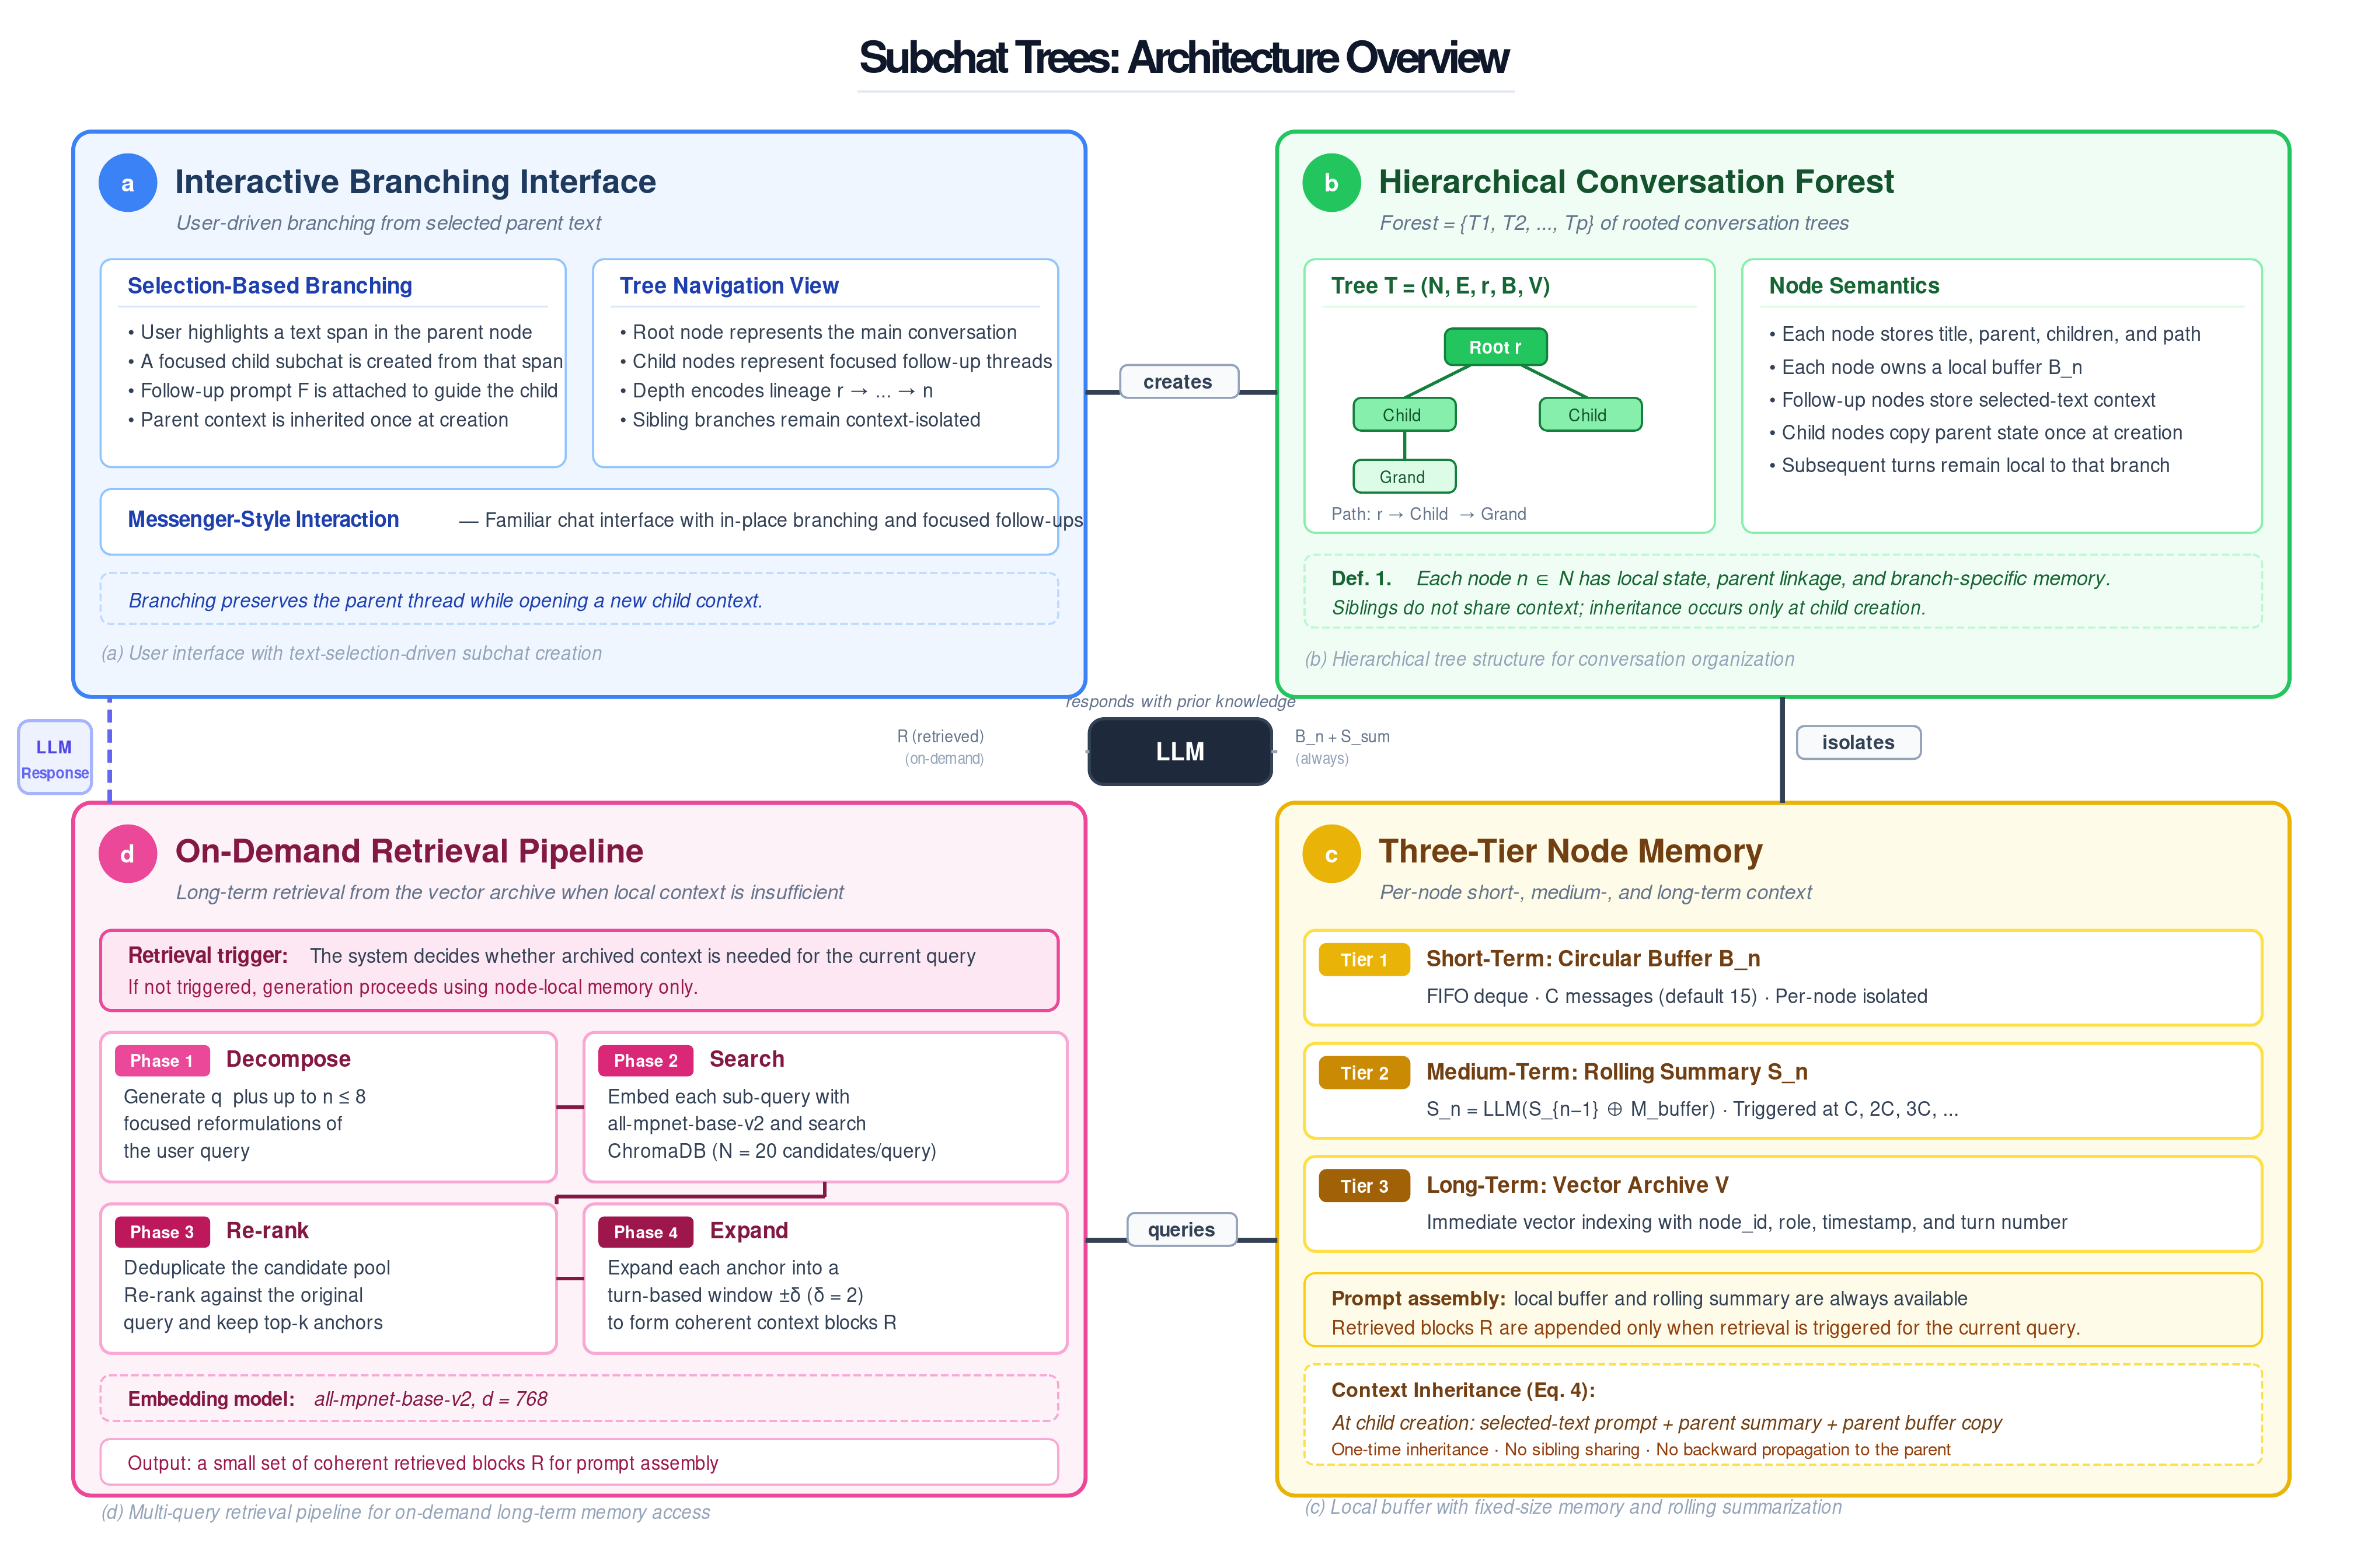
\includegraphics[width=1.15\textwidth]{diagrams/meth.png}
\caption{Overview of the SubchatTrees methodology showing four components: (a) hierarchical tree structure for conversation organization, (b) local buffer with fixed-size memory management, (c) global vector store for long-term archival and (d) multi-query RAG pipeline for context retrieval.}
\label{fig:methodology}
\end{figure}

\subsubsection{Hierarchical Conversation Tree Structure}\label{subsubsec:tree}

The system organizes conversations as hierarchical tree structures, where each node represents a distinct conversation thread with isolated context.





\begin{definition}[Conversation Tree]
A conversation tree $T$ is defined as a tuple of $(N, E, r, \mathcal{B}, \mathcal{V})$ here:
\begin{itemize}
    \item $N = \{n_1, n_2, \ldots, n_k\}$ set of conversation nodes,
    \item $E \subseteq N \times N$ set of directed parent$\to$child edges,
    \item $r \in N$  root node (main conversation),
    \item $\mathcal{B}: N \rightarrow B$ maps each node to its local buffer $B_i$,
    \item $\mathcal{V}: N \rightarrow \mathbb{R}^d$ maps each node's messages to $d$-dimensional embeddings space in a shared vector store.
\end{itemize}
\end{definition}

A \texttt{Forest} is a collection of independent trees $\mathcal{F} = \{T_1, T_2, \ldots, T_p\}$, allowing users to maintain isolate conversation threads (e.g., work projects, personal queries, research topics) without any cross-contamination. Figure~\ref{fig:forest} illustrates Hierarchical organization of Conversational Trees, composing the \texttt{conversation Forest}.





\begin{figure}[H]
\centering
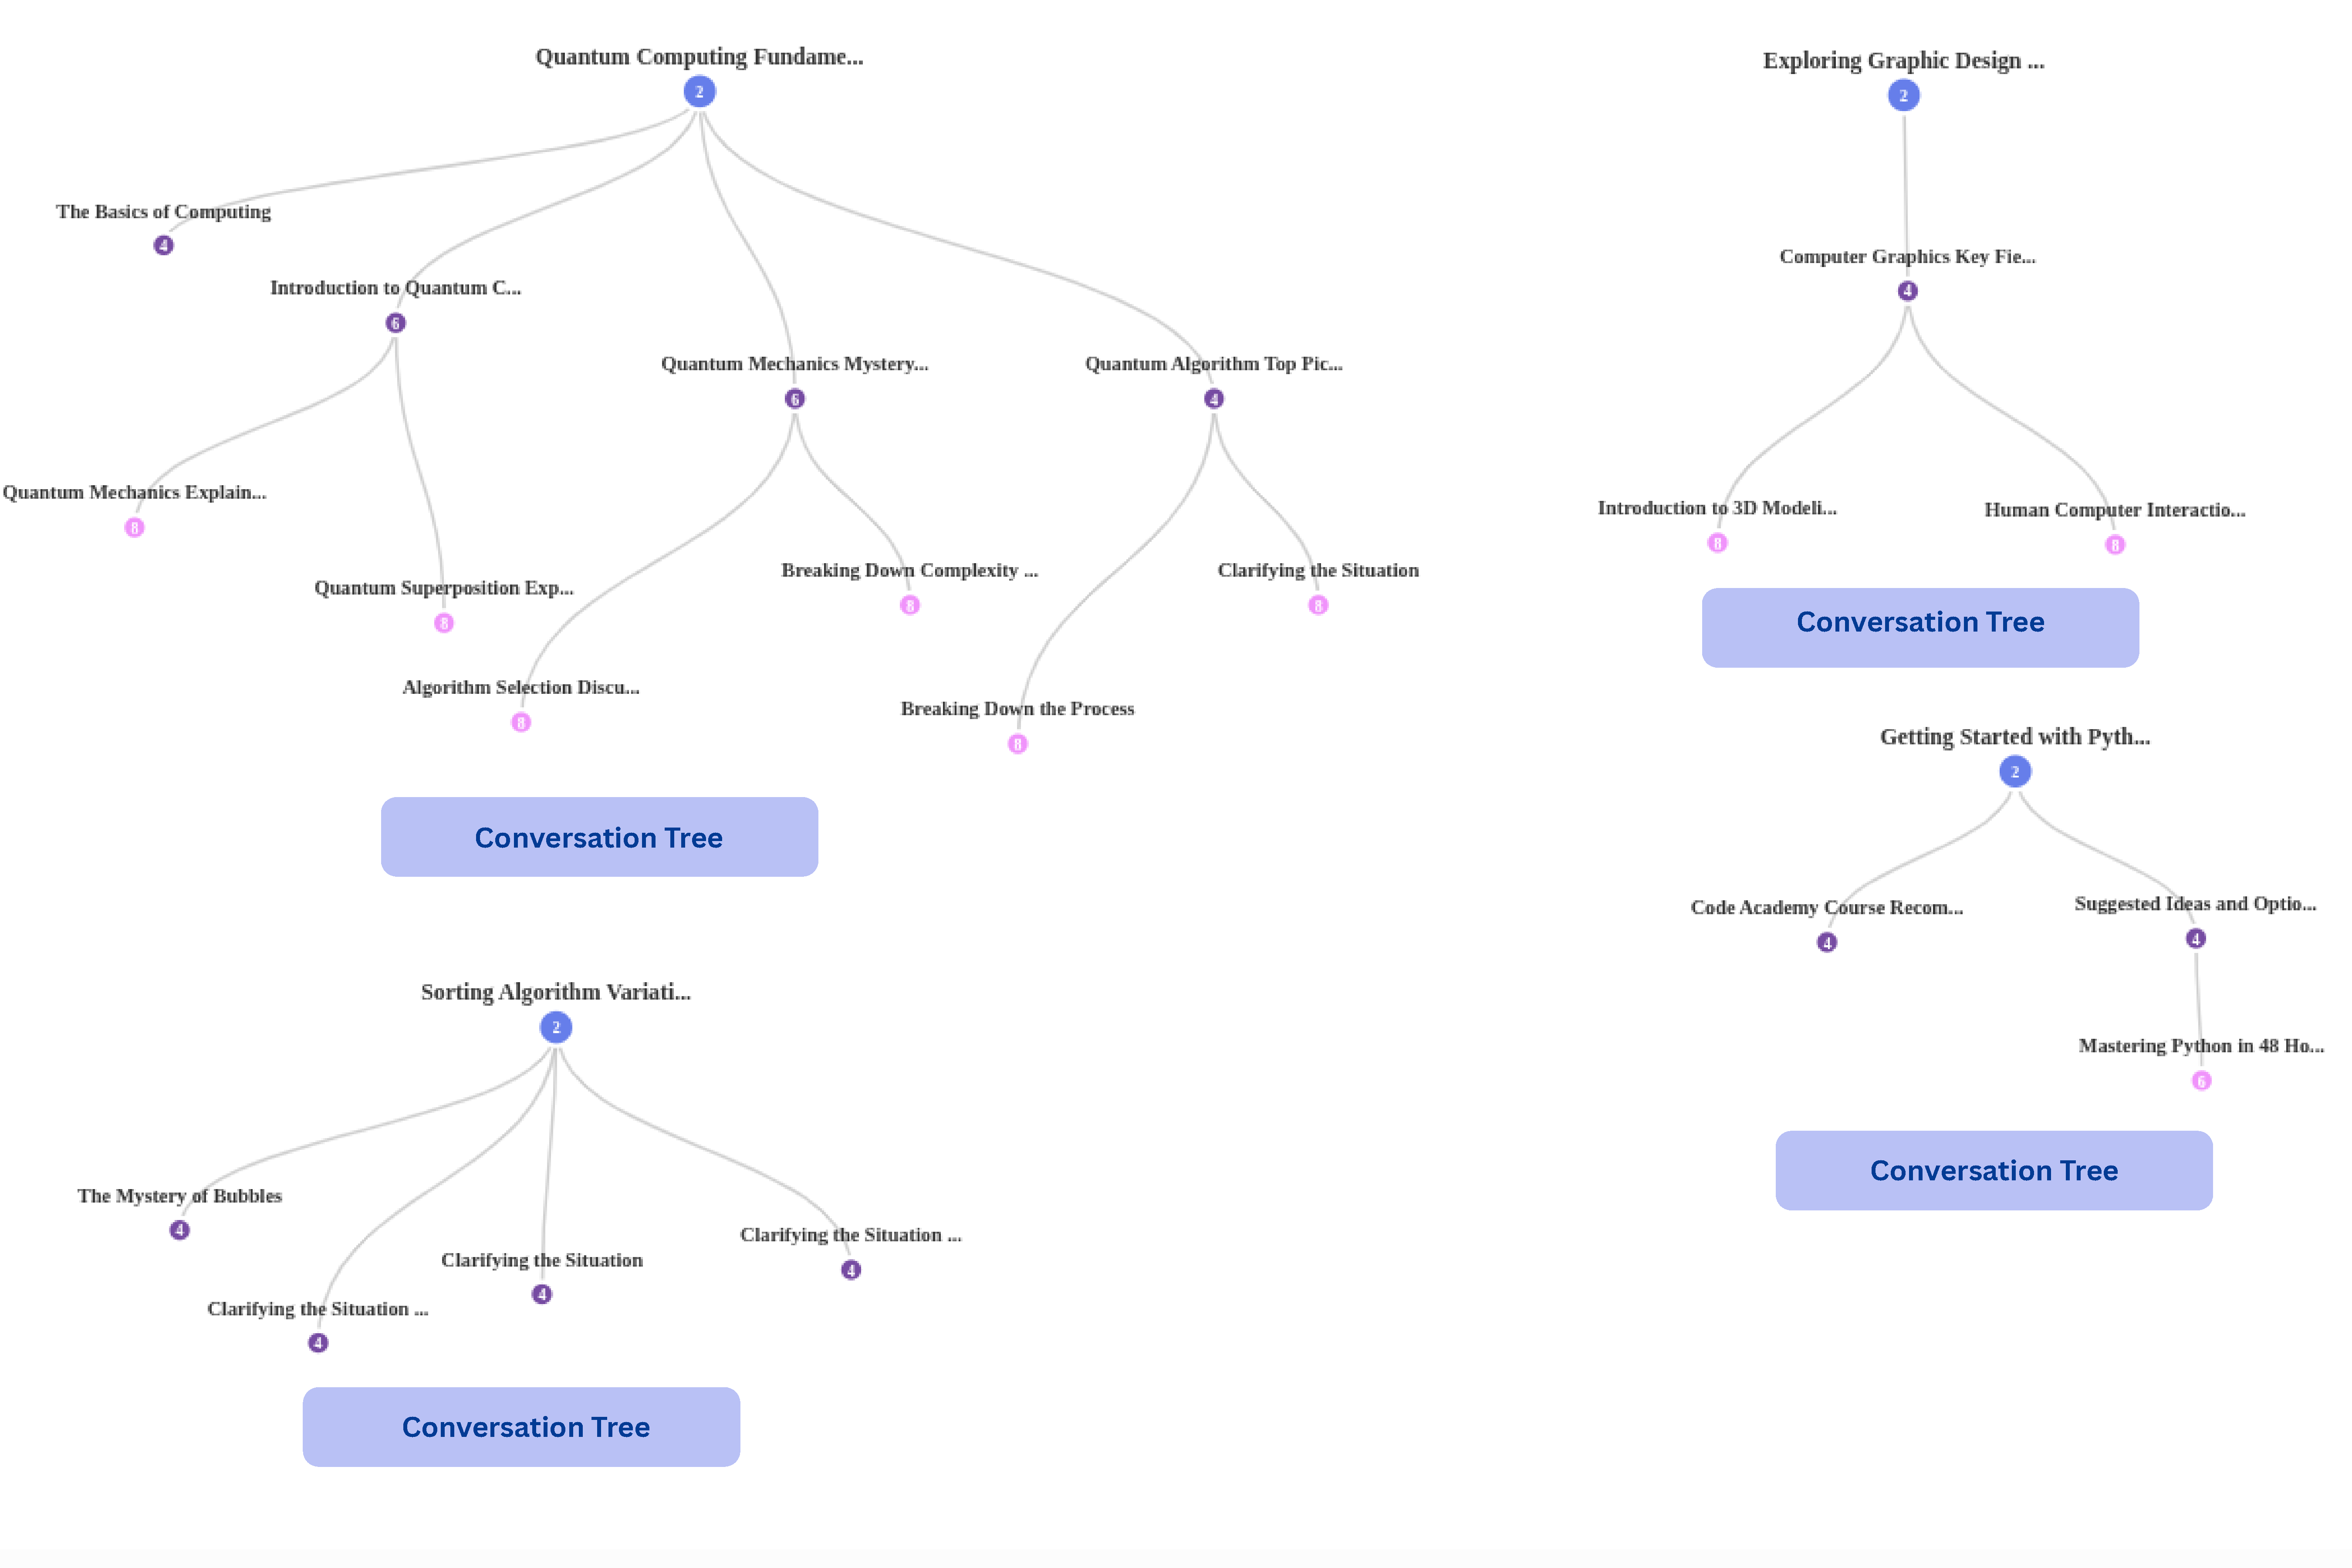
\includegraphics[width=\textwidth]{diagrams/conversation tree.pdf}
\caption{Tree view of a Conversation Forest showing multiple conversation branches. Each node represents a subchat with isolated context.}
\label{fig:forest}
\end{figure}

Each \texttt{Tree} node $n_i$ maintains its own:
\begin{enumerate}
    \item \textbf{Local Buffer} $B_i$: a circular deque with configurable capacity $C$ (default $C{=}20$ messages).
    \item \textbf{Node Metadata:} unique identifier (\texttt{node\_id}), title, parent reference, children pointers.
    \item \textbf{Follow-up Context:} user intent behind branch creation and context type (\texttt{follow\_up}, \texttt{new\_topic}, or \texttt{general}).
\end{enumerate}

\subsubsection{Memory Management Strategy}\label{subsubsec:memory}

The memory architecture is divided into three complementary tiers, illustrated in Figure~\ref{fig:memory}.

\begin{figure}[H]
\centering
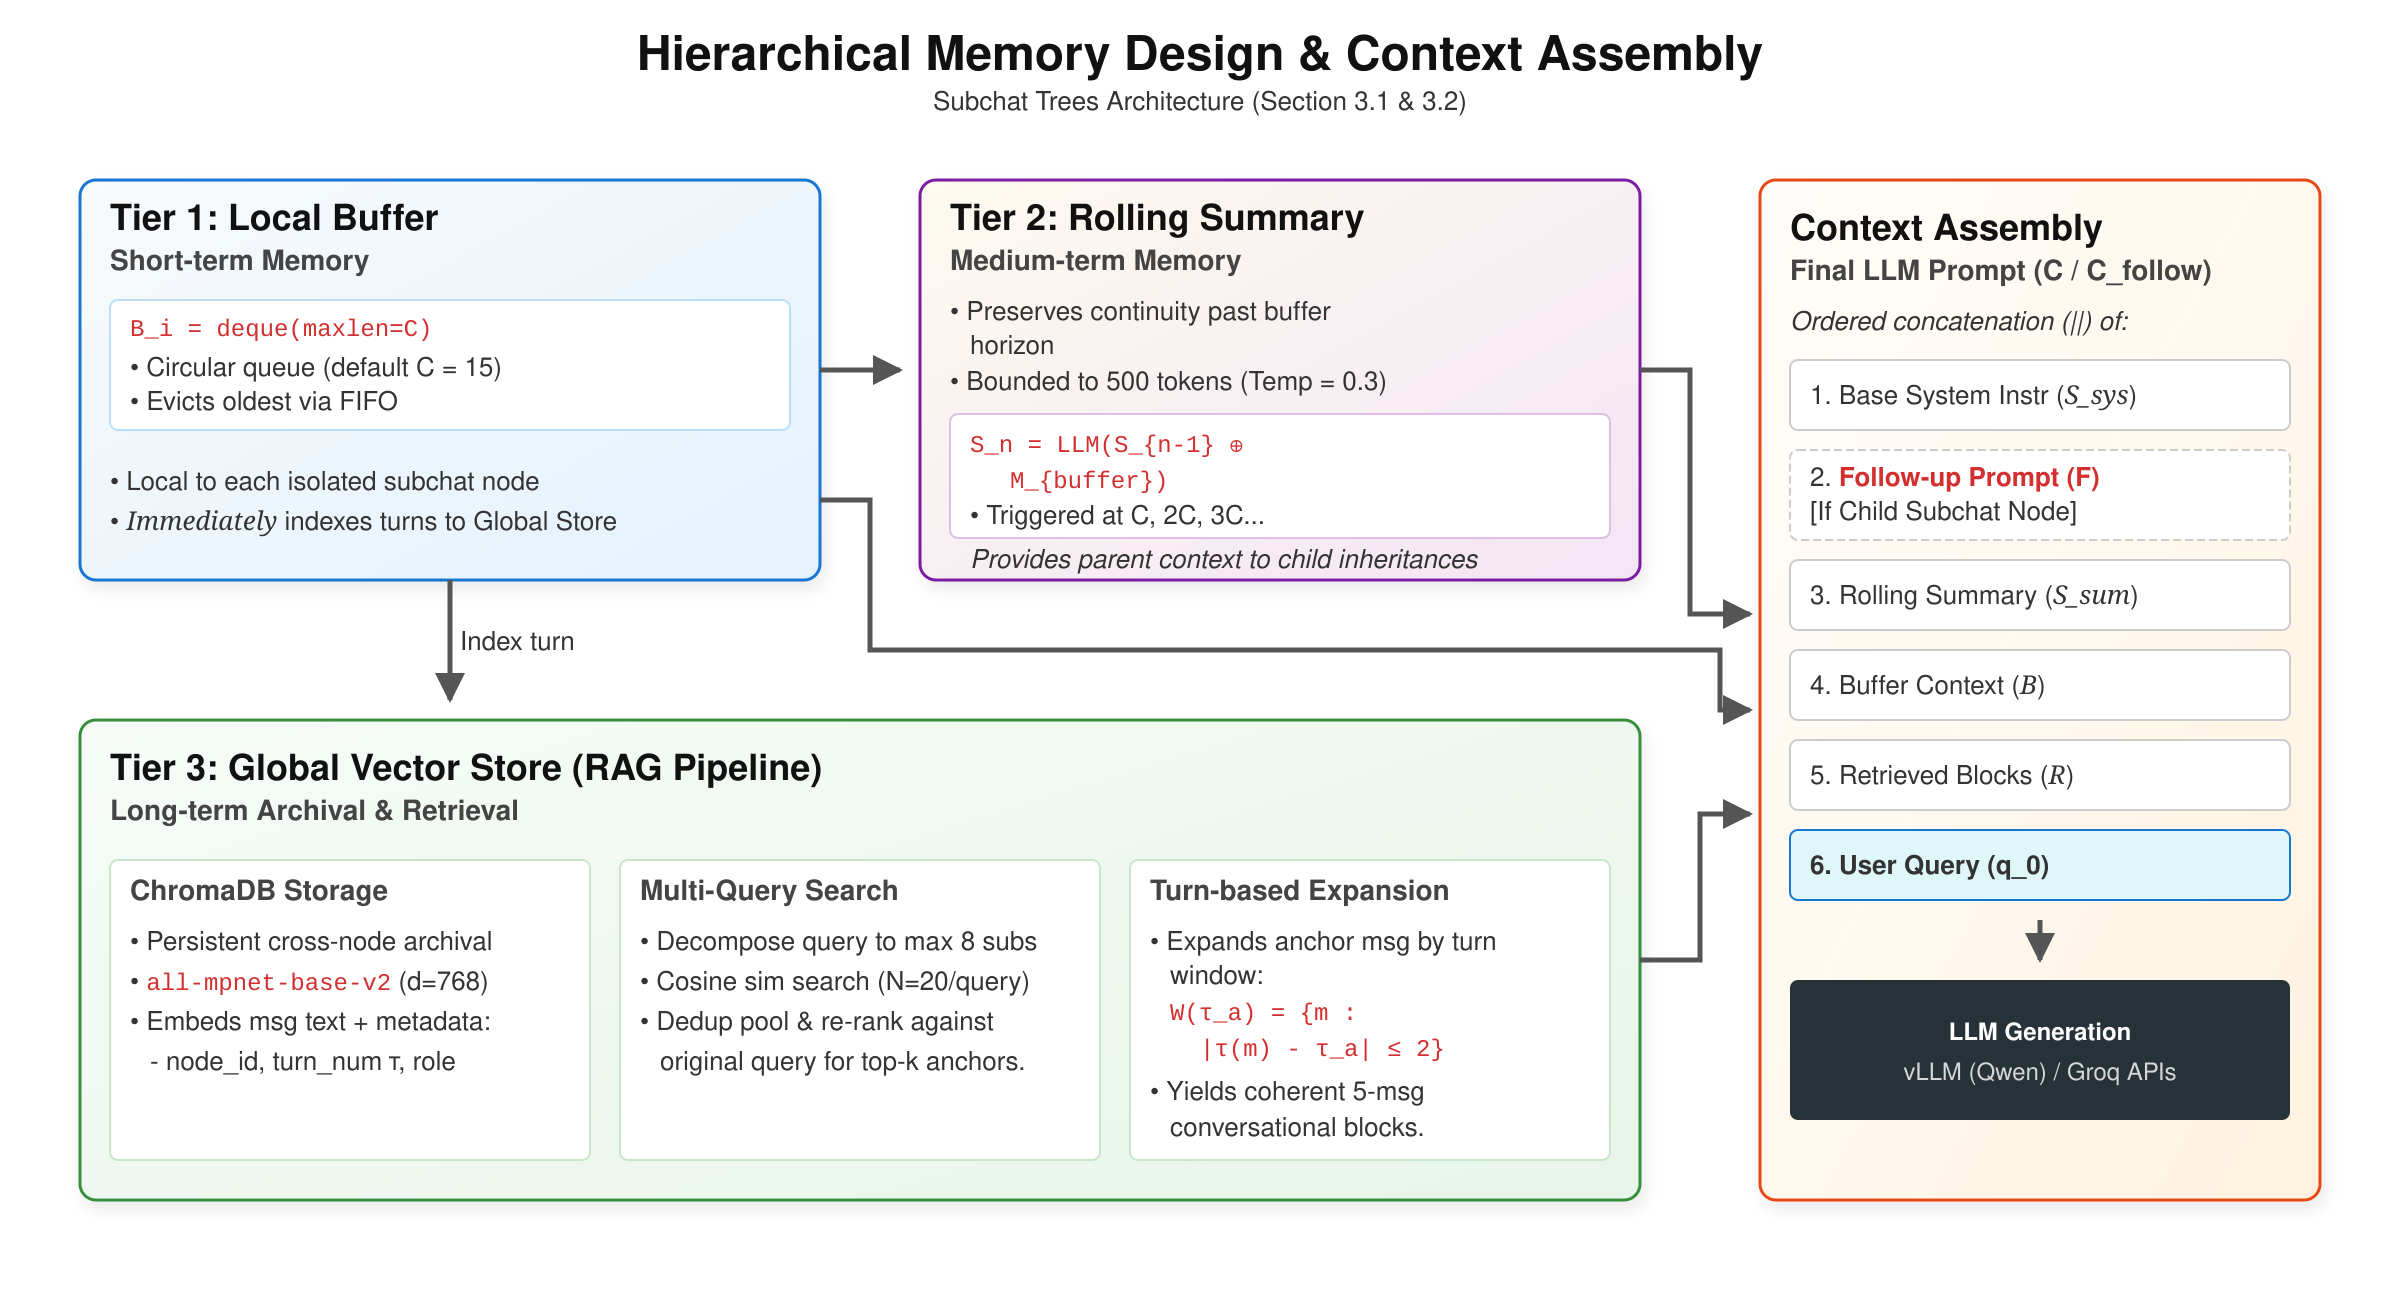
\includegraphics[width=0.85\textwidth]{diagrams/memory_design_academic.png}
\caption{Three-tier memory design showing the relationship between the LocalBuffer (circular deque), rolling summarization, and vector store archival.}
\label{fig:memory}
\end{figure}

\textbf{Tier~1: Local Buffer (Short-term Memory).}
Each node maintains a fixed-size circular buffer implemented as a \texttt{deque(maxlen=C)}:
\begin{equation}
B_i = \{(m_1, t_1), (m_2, t_2), \ldots, (m_C, t_C)\}
\label{eq:buffer}
\end{equation}
where $m_j$ is the $j$-th message, $t_j$ its timestamp, and $C$ the capacity. When $|B_i| > C$ or buffer limit reached, the oldest message is automatically evicted via FIFO policy. Crucially, messages are indexed to the global vector store \emph{immediately} upon addition (not upon eviction), ensuring up to date information availability during buffer turnover or node switching.

\textbf{Tier~2: Rolling Summarization (Medium-term Memory).}
To preserve semantic continuity beyond the buffer limit in long multi-turn conversation. A rolling summarization is triggered whenever the total message count reaches a multiple of the buffer size:
\begin{equation}
S_{n} = \text{LLM}_{\text{sum}}\!\left(S_{n-1} \oplus M_{\text{buffer}}\right), \quad \text{triggered at counts}\ C, 2C, 3C, \ldots
\label{eq:summary}
\end{equation}
where $S_n$ represent current summary, $S_{n-1}$ represent previous summary, $M_{\text{buffer}}$ is the complete set of messages currently in the buffer and $\oplus$ denotes concatenation. This dynamic triggering adapts to any buffer size without hard-coded thresholds. The summary is bounded at 500~tokens and generated at temperature $T{=}0.3$.

\textbf{Tier~3: Global Vector Store (Long-term Memory).}
All messages are embedded using \texttt{all-mpnet-base-v2} (SentenceTransformers, $d{=}768$) and stored in ChromaDB along with metadata:
\begin{equation}
\mathcal{V} = \left\{\left(\mathbf{e}(m),\; \text{meta}(m)\right) \;\middle|\; m \in \text{all messages}\right\}
\label{eq:vectorstore}
\end{equation}
where $\mathbf{e}(m) \in \mathbb{R}^{768}$ is the embedding and $\text{meta}(m)$ includes \texttt{node\_id}, \texttt{timestamp}, \texttt{role}, and \texttt{conversation\_title}. 

\subsubsection{Context Inheritance}\label{subsubsec:inheritance}

Creation of a child node $n_c$ from parent $n_p$:

\begin{equation}
\text{Context}(n_c) = \text{FollowUpPrompt}(n_c) \;\cup\; \text{BufferCopy}(n_p) \;\cup\; \text{SummaryInherit}(n_p)
\label{eq:inheritance}
\end{equation}

Specifically:
\begin{enumerate}
    \item \textbf{Buffer Inheritance:} All messages from the parent's buffer are copied into the child's buffer. This provides immediate conversational context.
    \item \textbf{Summary Inheritance:} The parent's rolling summary is also inherited. Transfering long term context to child.
    \item \textbf{Follow-up Prompt:} The selected text(parent's fragment) and user's intent (reason behind creating branch) are injected as a system message guiding the LLM's attention.
\end{enumerate}

The follow-up prompt is constructed as:
\begin{equation}
\text{FollowUpPrompt} = \texttt{``User selected:~''} \,\|\, s_{\text{sel}} \,\|\, \texttt{``~Focus on this.''}
\label{eq:followup}
\end{equation}

Here, subsequent messages in the child subchat do \emph{not} propagate back to the parent node, achieving bidirectional context isolation.

\subsubsection{Follow-up Mechanism}\label{subsubsec:followup_alg}

Algorithm~\ref{alg:subchat} formalizes the subchat creation process.

\begin{algorithm}[htbp]
\caption{Follow-up Subchat Creation}\label{alg:subchat}
\begin{algorithmic}[1]
\Require Parent node $n_p$, selected text $s_{\text{sel}}$, user query $q$, buffer size $C$
\Ensure Child node $n_c$ with isolated context
\State $n_c \gets \textsc{NewNode}(\text{parent}{=}n_p,\; C)$
\State $n_c.\text{context} \gets (s_{\text{sel}},\; \texttt{``follow\_up''})$
\State $\text{sys\_msg} \gets \textsc{BuildFollowUpPrompt}(s_{\text{sel}})$
\For{each message $m \in n_p.\text{buffer}$}
    \State $n_c.\text{buffer}.\textsc{Add}(m.\text{role},\; m.\text{text})$ \Comment{Inherit parent context}
\EndFor
\State $n_c.\text{summary} \gets n_p.\text{summary}$ \Comment{Inherit rolling summary}
\State $r \gets \text{LLM}\!\left(\text{sys\_msg} \;\|\; n_c.\text{buffer} \;\|\; q\right)$
\State $n_c.\text{buffer}.\textsc{Add}(\texttt{``user''},\; q)$
\State $n_c.\text{buffer}.\textsc{Add}(\texttt{``assistant''},\; r)$
\State \Return $n_c$
\end{algorithmic}
\end{algorithm}

\subsection{Vector Memory and RAG Pipeline}\label{subsec:rag}

The global vector store serves as long-term memory. It enables retrieval of relevant context from any point in any branch.

\subsubsection{Multi-Query Decomposition and Retrieval}\label{subsubsec:decomposition}

A single user query rarely captures all retrievable facets of a topic. Thus, the retrieval pipeline uses a four-phase process, 1. sub-query generation, 2. embedding-based vector search, 3. deduplication and 4. re-ranking. Figure~\ref{fig:retrieval_pipeline} illustrates the full flow.

\paragraph{Sub-Query Generation.}
We prompt the LLM (Groq API, temperature~$T{=}0.3$) with intent-specific templates to decompose~$q$ into a set of sub-queries $Q = \{q_0, q_1, \dots, q_{n-1}\}$, where $q_0 = q$ is the original query and $q_1 \dots q_{n-1}$ are alternative query versions targeting related concepts, specific entities, or broader context ($n \leq 8$).






\paragraph{Embedding and Vector Search.}
Each sub-query~$q_i$ is independently embedded using the \texttt{all-mpnet-base-v2} sentence-transformer model~\cite{reimers2019sentencebert}, producing a dense vector $e(q_i) \in \mathbb{R}^{768}$. Every indexed message in the system has been embedded with the same model and stored in a persistent ChromaDB~\cite{chromadb} collection. Each stored message also includes metadata fields such as \texttt{node\_id}, \texttt{role}, \texttt{timestamp}, \texttt{turn\_number}~$\tau$, \texttt{title}, and an \texttt{archived} flag. A cosine-similarity search retrieves top $N{=}20$ candidate messages per sub-query from the collection.

\paragraph{Deduplication.}
Multiple sub-queries can return the same message. Thus, the system  deduplicate per sub-query (by content and message identifier), retaining at most $u = 5$ unique results each. A shared \emph{seen} set further removes cross-query duplicates. The candidate pool is then:
\begin{equation}
\mathcal{P} = \bigcup_{i=0}^{n-1} R_i, \quad |R_i| \leq u, \quad |\mathcal{P}| \leq n \cdot u
\label{eq:candidate_pool}
\end{equation}
where $R_i$ denotes the unique results for sub-query~$q_i$. A cosine-similarity re-ranking scores every candidate in~$\mathcal{P}$ against the original query~$q_0$ and returns the top-$k$ anchor messages ($k \in [3, 10]$, default~5) for downstream turn-based expansion (Section~\ref{subsubsec:window}).

\begin{figure}[H]
\centering

\includegraphics[width=\textwidth, keepaspectratio]{diagrams/retrieval_pipeline.png}
\caption{End-to-end retrieval pipeline. \textbf{Phase~1}: LLM-based sub-query generation decomposes the user query into up to $n \leq 8$ sub-queries. \textbf{Phase~2}: each sub-query is embedded via \texttt{all-mpnet-base-v2} ($d{=}768$) and dispatched to ChromaDB for cosine search ($N{=}20$ candidates each), then deduplicated to $u{=}5$ unique results per sub-query. \textbf{Phase~3}: all anchor candidates are re-ranked by cosine similarity to the original query~$q_0$; top-$k$ are selected. \textbf{Phase~4}: each winning anchor expands $\pm\delta$ turns ($\delta{=}2$) into a coherent conversational block (Eq.~\ref{eq:window}). The resulting~$k$ blocks are injected into the LLM prompt.}
\label{fig:retrieval_pipeline}
\end{figure}

\subsubsection{Context Window Retrieval}\label{subsubsec:window}

A retrieved message in isolation often lacks the conversational context necessary for coherent understanding. A na\"ive approach would define a temporal window (e.g.,\ $\pm 60$\,s around the anchor), but user response latencies are inconsistent and unpredictable---a reader may pause for seconds or minutes before replying---making time-based windows unreliable. We Therefore define a \emph{turn-based} context window anchored on conversational sequence.

Each message~$m$ is indexed with a monotonically increasing turn number $\tau(m)$ within its node. For an anchor message with turn number~$\tau_a$, the context window is:
\begin{equation}
W(\tau_a) = \left\{m \in M_{n} : |\tau(m) - \tau_a| \leq \delta\right\}
\label{eq:window}
\end{equation}
where $M_n$ is the set of all indexed messages in node~$n$ and $\delta = 2$ (i.e.,\ two turns before and two turns after the anchor). This yields at most $2\delta + 1 = 5$ messages per anchor regardless of the time elapsed between turns. As with temporal windows, we exclude any message still held in the active buffer:
\begin{equation}
W_{\mathrm{filtered}}(\tau_a) = W(\tau_a) \setminus B
\label{eq:window_filtered}
\end{equation}
here, $B$ denotes the current buffer contents.

Context expansion is applied \emph{after} re-ranking rather than before. The retrieval pipeline first re-ranks all deduplicated anchor candidates by cosine similarity to the original query~$q_0$ and selects the top-$k$ anchors ($k \in [3, 10]$, default~5). Only then does each winning anchor expand into its $\pm\delta$ turn window. This "\emph{rank-then-expand}" ordering ensures that neighbouring  messages never compete with anchors during ranking. Instead of that, each anchor is delivered to the LLM as a coherent conversational block rather than as scattered fragments interleaved with unrelated messages. Neighbour messages receive a discounted relevance score of $0.8 \times$ the anchor score. This helps preserving the distinction between directly matched content and its surrounding narrative.

\subsubsection{Context Assembly}\label{subsubsec:assembly}

The final prompt sent to the LLM is an ordered sequence of messages. Its composition differs depending on whether the active node is a \emph{root-level} conversation or a \emph{follow-up subchat}. Figure~\ref{fig:dataflow} illustrates both paths.

\begin{figure}[H]
\centering
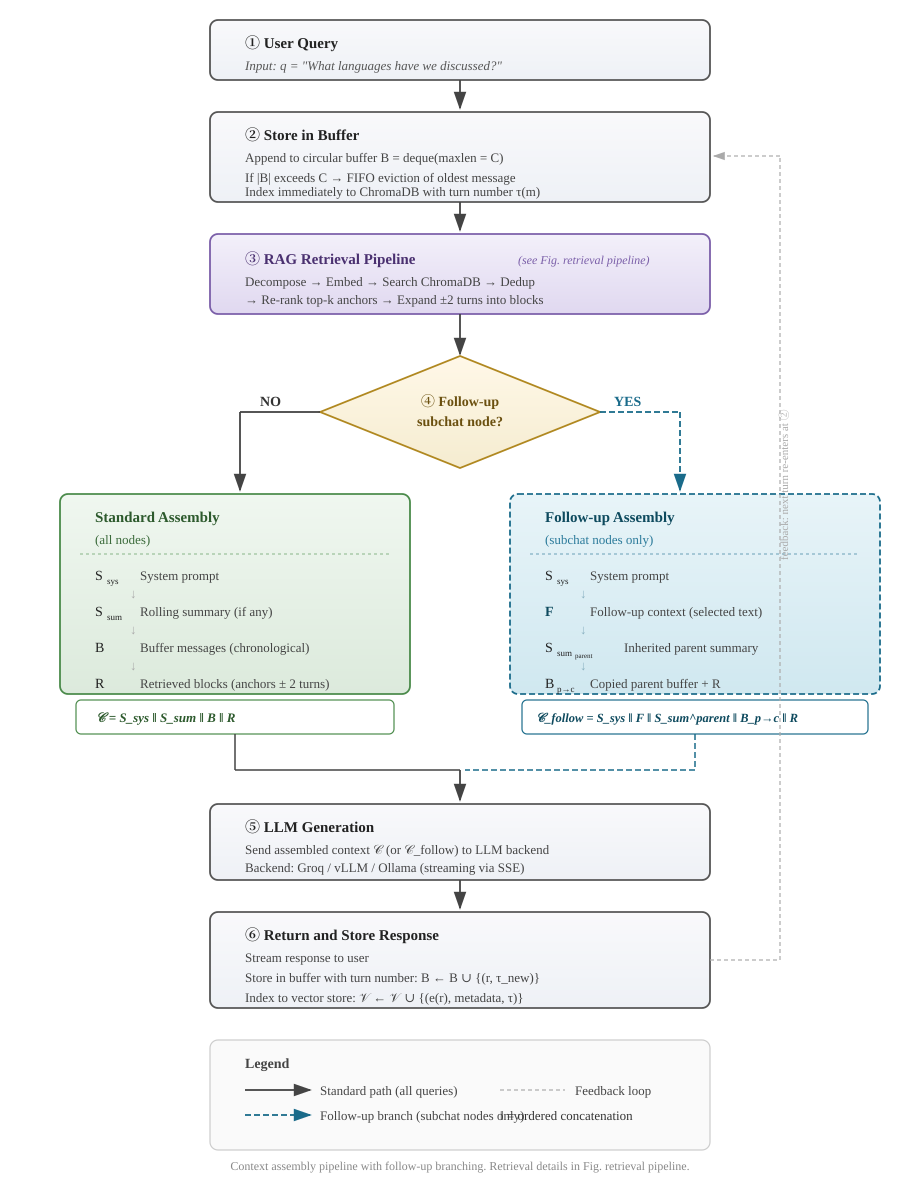
\includegraphics[width=\textwidth, keepaspectratio]{diagrams/context_assembly_pipeline.png}
\caption{Context assembly pipeline. The user query is buffered (\textcircled{1}--\textcircled{2}) and passed through the RAG retrieval pipeline (\textcircled{3}; detailed in Figure~\ref{fig:retrieval_pipeline}), which returns coherent context blocks~$R$. At step~\textcircled{4} the pipeline branches: root-level nodes follow the \emph{standard} path (solid arrows, Eq.~\ref{eq:context_standard}), while follow-up subchat nodes additionally inject the selected-text prompt~$F$ and the inherited parent summary $S_{\mathrm{sum}}^{\,\mathrm{parent}}$ (dashed arrows, Eq.~\ref{eq:context_followup}). Both paths converge at step~\textcircled{5} for LLM generation, after which the response is stored back in the buffer and vector store (\textcircled{6}).}
\label{fig:dataflow}
\end{figure}

\paragraph{Standard Assembly (all nodes).}
Every query passes through the seven-step RAG pipeline described above. The assembled prompt takes the form:
\begin{equation}
\mathcal{C} = S_{\mathrm{sys}} \;\|\; S_{\mathrm{sum}} \;\|\; B \;\|\; R
\label{eq:context_standard}
\end{equation}
where $S_{\mathrm{sys}}$ is the base system instruction, $S_{\mathrm{sum}}$ is the node's rolling summary (omitted if none exists), $B$ is the circular buffer (recent turns in chronological order), $R$ is the set of retrieved messages returned by the RAG pipeline (empty when retrieval is not triggered), and $\|$ denotes ordered concatenation.

\paragraph{Follow-up Assembly (subchat nodes).}
When a user selects text in a parent conversation and creates a subchat. The child node inherits three artifacts from its parent at creation time:
\begin{enumerate}
    \item \textbf{User intent prompt.} The text the user highlighted, along with users intent, is wrapped in a system message directing the model to focus on that specific topic.
    \item \textbf{Inherited summary.} The parent's rolling summary is copied to the child, providing long term context.
    \item \textbf{Parent buffer messages.} All messages currently in the parent's circular buffer are copied into the child's buffer. This ensures the child begins with the full recent context of the parent conversation.
\end{enumerate}
The resulting prompt becomes:
\begin{equation}
\mathcal{C}_{\mathrm{follow}} = S_{\mathrm{sys}} \;\|\; F \;\|\; S_{\mathrm{sum}}^{\,\mathrm{parent}} \;\|\; B_{\mathrm{parent} \to \mathrm{child}} \;\|\; R
\label{eq:context_followup}
\end{equation}
where $F$ is the follow-up context, $S_{\mathrm{sum}}^{\,\mathrm{parent}}$ is the inherited parent summary, and $B_{\mathrm{parent} \to \mathrm{child}}$ denotes the child's buffer initialized with the parent's messages. As the child conversation progresses, new turns are appended to this buffer (evicting older ones via FIFO), and its own rolling summary gradually replaces the inherited one, ensuring continuity while allowing topic divergence. But parent's state remain unchanged.

\subsection{User Interface}\label{subsec:ui}

\paragraph{Design Rationale.}
The interface deliberately adopts a messenger-style layout---a familiar paradigm shared by WhatsApp, iMessage, and Slack---so that users can transfer existing mental models to the new system without additional learning overhead~\cite{nielsen1994usability}. By anchoring interaction in a well-understood pattern (send a message, receive a reply), the cognitive cost of the novel \emph{subchat} mechanism is kept low.

\paragraph{The Problem with Linear Chat.}
Conventional LLM chat interfaces present all exchanges in a single, chronologically ordered thread. As conversations grow in length or branch across topics, this layout introduces several usability failures: (i)~users must scroll extensively to relocate earlier context, (ii)~there is no affordance for branching---returning to a prior topic forces the user to re-state context or risk contaminating the current thread, and (iii)~the model's fixed context window silently evicts earlier turns, creating an invisible boundary between what the user remembers and what the model can still ``see.'' These issues compound in exploratory or multi-topic sessions.

\paragraph{Subchat Trees as a Solution.}
Our interface exposes the underlying tree structure through two complementary views (Figure~\ref{fig:ui}): a collapsible \emph{tree navigator} on the left and a focused \emph{chat panel} on the right. Users create a subchat by selecting any text in the chat panel and clicking a single button; the new subchat inherits relevant context (Section~\ref{subsubsec:assembly}) without disrupting the parent conversation. This design follows the principle of \emph{progressive disclosure}~\cite{norman2013design}: the default view is a simple chat, but richer structure (branching, parallel follow-ups, hierarchical navigation) is available on demand.

\begin{figure}[H]
\centering
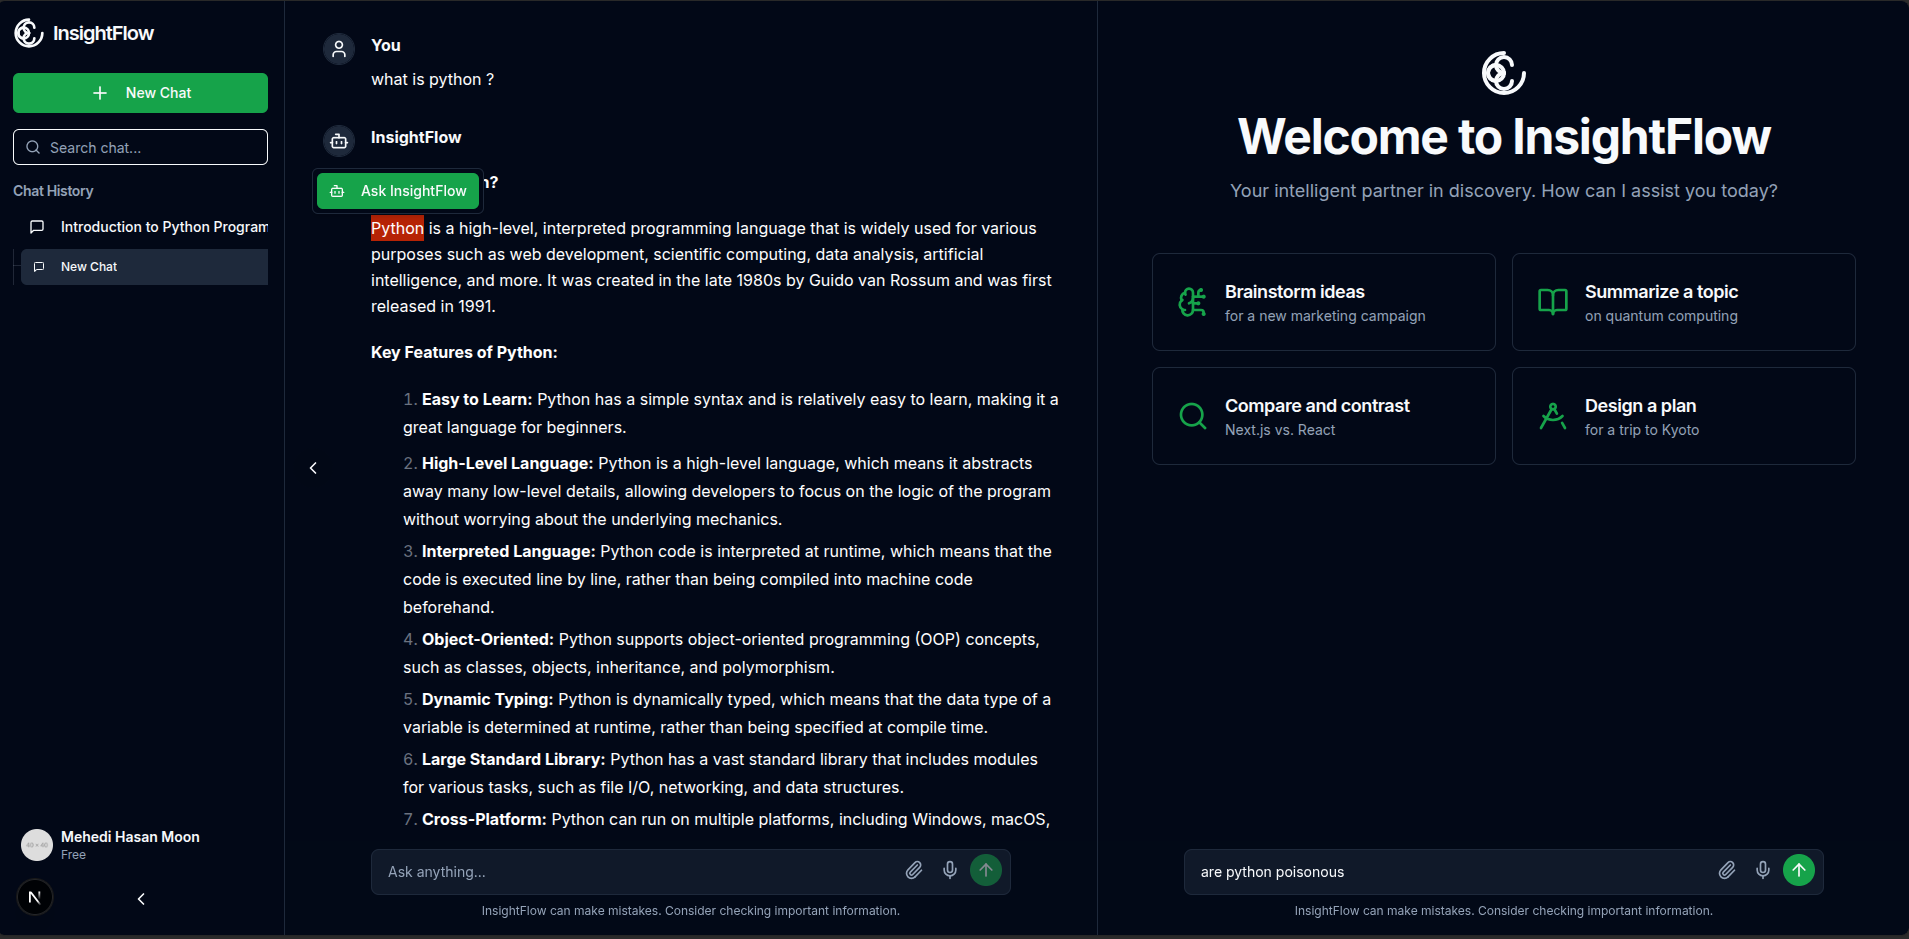
\includegraphics[width=0.9\textwidth]{diagrams/frontend.png}
\caption{User interface: (left) the conversation forest tree view with expandable nodes, and (right) the chat panel with text selection for one-click subchat creation.}
\label{fig:ui}
\end{figure}

Key affordances include: (i)~breadcrumb navigation showing the path from root to the active subchat, (ii)~visual indicators for inherited context and active retrieval status, (iii)~parallel follow-ups that let users explore multiple branches of a topic simultaneously, and (iv)~real-time token streaming via Server-Sent Events across multiple LLM backends (Groq, vLLM, Ollama).

\subsection{Baseline System}\label{subsec:baseline}

For comparison, we implement a linear chat baseline:
\begin{itemize}
    \item Single conversation thread with a shared circular buffer ($C$ messages, FIFO eviction).
    \item All topics share the same context window---no isolation mechanism.
    \item Identical LLM backend, embedding model, and temperature settings.
\end{itemize}
Both systems use the same buffer capacity $C$ in each experiment, isolating the effect of conversation structure.

\subsection{Evaluation Framework}\label{subsec:eval}

\subsubsection{Dataset Design}\label{subsubsec:dataset}

The final evaluation dataset is \texttt{VBRI\_merged.json}, a 352-turn stress-test conversation derived from five real LMSYS-Chat-1M conversations~\cite{zheng2024lmsyschat} produced by vicuna-13b, alpaca-13b, and koala-13b. Each source conversation was first transformed into a replayable hierarchical script with explicit topic labels, subchat actions, selected-text spans, and required response-prefix labels. The final benchmark then merges these five scripts into a single interleaved conversation.

\textbf{Variable-Block Randomized Interleaving (VBRI).}
To stress-test context isolation and recall under realistic multi-topic switching patterns, we developed a merged evaluation scenario using Variable-Block Randomized Interleaving (VBRI). VBRI simulates sessions where users return to earlier topics after short bursts of unrelated discussion while preserving the temporal logic of each original conversation.

The VBRI algorithm operates as follows:
\begin{enumerate}
    \item \textbf{Source-Level FIFO:} Each of the five source scenarios maintains a local queue of ordered blocks. On each iteration, the algorithm selects one source scenario and removes the next block from that source's queue. This guarantees that the original temporal order within every source conversation is preserved.
    \item \textbf{Variable Blocks:} Consecutive same-topic turns are grouped into blocks. Blocks longer than $b_{\max}{=}4$ are split into smaller ordered sub-blocks, preserving short local coherence while preventing one topic from dominating the merged stream.
    \item \textbf{Temporal Preservation:} Within each source scenario, turns maintain their original sequential order. This preserves logical dependencies (e.g., follow-up questions must appear after their referents) while allowing cross-scenario interleaving.
    \item \textbf{Topic Return Dynamics:} With probability $p_{\text{ret}}{=}0.3$, the next block is drawn from the same source as the previous block; otherwise, another active source is selected uniformly. This creates bursty topic revisitation rather than complete random shuffling.
    \item \textbf{Deterministic Reproducibility:} A fixed random seed (42) ensures identical interleaving across experimental runs.
\end{enumerate}

The resulting merged dataset contains 309 original conversation turns spanning 59 distinct LMSYS-derived topics. It contains 91 topic switches, 64 source-conversation switches, 25 topic returns, and no temporal-order violations within any source conversation.

\textbf{Summarization Probes.}
After the 309 ordinary turns, the dataset appends 43 summarization-probe steps, producing 352 total steps. These probes are added only for topics with at least three user turns. Each probe asks the model to summarize what was discussed about one topic, for example: \texttt{Summarize everything we have discussed about ai chat tools. Include all key points, details, and questions that were raised.} The purpose is to test topic-level context retention after a long interleaved conversation, not only immediate topic-prefix selection. In the linear baseline, every probe is sent to the same main conversation node, where all topics have been mixed into one shared history. In Subchat Trees, probes are routed to the relevant topic subchat branch , so the model retrieves from a branch whose local buffer, summary, and vector memory are focused on one topic. This design directly tests whether dividing roles across topic-specific nodes improves the model's ability to recall earlier information.

\textbf{Dataset Structure.}
The dataset is encoded as a JSON file with the following schema:
\begin{itemize}
    \item \texttt{scenario\_name}: Unique identifier for the scenario.
    \item \texttt{conversations}: Ordered list of conversation steps.
    \item Each step contains:
    \begin{itemize}
        \item \texttt{step}: Integer turn number (1-indexed).
        \item \texttt{context}: Ground-truth topic label (e.g., \texttt{``indian\_history''}, \texttt{``astrology''}).
        \item \texttt{message}: Raw user query.
        \item \texttt{node\_type}: Target subchat identifier (e.g., \texttt{``main''}, \texttt{``subchat\_indian\_history''}).
        \item \texttt{action}: Operation type (\texttt{create\_subchat}, \texttt{switch\_node}, or implicit continuation).
        \item \texttt{selected\_text}: (Optional) Text fragment selected for follow-up subchat creation.
        \item \texttt{subchat\_title}: (Optional) Human-readable title for new subchats.
        \item \texttt{parent\_node\_type}: (Optional) Parent node for hierarchical subchat creation.
        \item \texttt{is\_recall\_probe}: (Optional) Boolean marker for appended summarization-probe steps.
        \item \texttt{probe\_topic}: (Optional) Topic being tested by a summarization probe.
        \item \texttt{probe\_target\_node}: (Optional) Target node for a summarization probe.
    \end{itemize}
\end{itemize}

For example, a step from the merged interleaved dataset:
\begin{verbatim}
{
  "step": 45,
  "context": "indian_legal_family",
  "message": "Can you explain the Hindu Succession Act?",
  "node_type": "subchat_indian_legal_family",
  "action": "create_subchat",
  "selected_text": "Indian legal framework",
  "subchat_title": "Hindu Succession Act Discussion",
  "parent_node_type": "subchat_indian_legal"
}
\end{verbatim}

This structure enables deterministic replay: the test harness iterates through steps sequentially, performs the specified action (create subchat, switch node), sends the user message to the target node, and scores the response against the ground-truth context label.

Summarization probes use the same replay mechanism. They are encoded as \texttt{switch\_node} steps so the baseline can ask the probe in its single main node, while Subchat Trees can ask the same probe in the topic-specific node indicated by \texttt{probe\_target\_node}. Probe responses are excluded from topic-prefix isolation counts and are used only for recall scoring.

In the baseline condition, all steps are replayed into one linear conversation node (MAIN) regardless of their annotated \texttt{node\_type}. In the Subchat Trees condition, \texttt{create\_subchat} steps instantiate child nodes under the annotated parent, \texttt{switch\_node} steps route the next message to an existing node, and ordinary continuation steps remain in the current annotated node. This means both conditions receive the same user messages in the same order; only the context organization differs.

Table~\ref{tab:scenarios} summarizes the dataset provenance using the original LMSYS conversation identifiers. The table reports the five source conversations that form \texttt{merged\_vbri\_temporal}, the final dataset used in the Kaggle run.

\begin{table}[htbp]
\caption{Conversation-level provenance for the final VBRI dataset. Turns denote replay turns contributed to \texttt{merged\_realistic\_interleaved.json}, excluding appended recall probes.}\label{tab:scenarios}
\centering
\scriptsize
\setlength{\tabcolsep}{4pt}
\begin{tabular*}{\textwidth}{@{\extracolsep\fill}p{3.2cm}ccp{6.0cm}@{}}
\toprule
\textbf{Source Conversation ID} & \textbf{Turns} & \textbf{Topics} & \textbf{Source Stress Pattern} \\
\midrule
\texttt{22807e655dd04}\newline\texttt{2348cb0ee402}\newline\texttt{3672e70} & 52 & 4 & Persona roleplay, role reversal, LLM-knowledge questions, and Twenty Questions game-state confusion \\
\texttt{6c4992f0aed04}\newline\texttt{dd3bf9a4bc225}\newline\texttt{bb4fb0} & 62 & 11 & Medical discussion, AI consciousness, repetitive-loop failure, pandemic safety, and literature analysis \\
\texttt{8d10c143f8fc4}\newline\texttt{a7599a5a1877}\newline\texttt{8fec112} & 77 & 17 & DSP, C programming, medical genetics, Linux audio, physics, science fiction, geography, and games \\
\texttt{eaf06f12a1d74}\newline\texttt{e5ca30a7ca94}\newline\texttt{a7c4128} & 53 & 8 & Cookie recipes, recipe-halving math errors, argumentative correction, jokes, and emoji game turns \\
\texttt{ec366fd3e4b54}\newline\texttt{82e8acac750f}\newline\texttt{9b3b55b} & 64 & 19 & Explicit context resets across Indian history, LSAT reasoning, law, nutrition, astrology, travel, therapy, and chess \\
\midrule
\textbf{\texttt{merged\_vbri\_temporal}} & \textbf{309} & \textbf{59} & \textbf{Final interleaved benchmark used for context-isolation scoring and recall probes} \\
\botrule
\end{tabular*}
\end{table}

The final replay contains 309 ordinary conversation turns and 59 normalized topic labels. Its replay annotations create 51 subchats. The probe-injected version appends 43 recall probes, producing 352 total steps; those probes are not counted as ordinary conversation turns in Table~\ref{tab:scenarios}.

\subsubsection{Evaluation Matrices}\label{subsubsec:metrics}

The evaluation reports four complementary matrices. Each matrix measures a different part of the study: whether a conversation system can keep the right topic active, retain the content of that topic, how  efficiently the system is and can we reduce retrieval rate.

\textbf{Context Isolation Matrix.}
The context isolation matrix measures turn-level topic control. For each ordinary replay turn $t$, the dataset provides a ground-truth topic label $\tau_t$. The model response is scored by extracting the leading topic prefix, denoted $\hat{\tau}_t$. A turn is correct when $\hat{\tau}_t=\tau_t$; otherwise it is counted as context pollution because the response has been assigned to the wrong conversational context. This metric therefore evaluates both memory of the active topic and the ability to match the user query to the correct topic state.

For each topic $\tau_i$, we build a one-vs-rest confusion matrix:
\begin{itemize}
    \item $\text{TP}_i$: $\tau_i$ was expected and the response was labeled as $\tau_i$.
    \item $\text{FP}_i$: another topic was expected, but the response was labeled as $\tau_i$.
    \item $\text{FN}_i$: $\tau_i$ was expected, but the response was labeled as another topic or as unknown.
\end{itemize}
The support $n_i$ is the number of turns whose ground-truth topic is $\tau_i$. Per-topic precision, recall, and F1 are:
\begin{equation}
P_i = \frac{\text{TP}_i}{\text{TP}_i + \text{FP}_i}, \quad
R_i = \frac{\text{TP}_i}{\text{TP}_i + \text{FN}_i}, \quad
F1_i = \frac{2P_iR_i}{P_i + R_i}.
\label{eq:per_topic_metrics}
\end{equation}
The main table reports support-weighted averages:
\begin{equation}
\text{Precision}_w = \sum_i \frac{n_i}{\sum_j n_j} P_i, \quad
\text{Recall}_w = \sum_i \frac{n_i}{\sum_j n_j} R_i, \quad
\text{F1}_w = \sum_i \frac{n_i}{\sum_j n_j} F1_i.
\label{eq:weighted_isolation}
\end{equation}
Macro averages are also computed by giving every topic equal weight. Weighted scores show performance over the full replay distribution, while macro scores check whether improvements are not limited to high-frequency topics.

Overall accuracy and pollution rate are computed over all ordinary replay turns:
\begin{equation}
\text{Accuracy} = \frac{|\{t:\hat{\tau}_t=\tau_t\}|}{N}, \quad
\text{Pollution Rate} = 1-\text{Accuracy},
\label{eq:accuracy_pollution}
\end{equation}
where $N$ is the number of ordinary replay turns. A lower pollution rate means fewer responses were contaminated by another topic.

\textbf{Topic Recall Matrix.}
The topic recall matrix evaluates content retention rather than only topic-label selection. After the 309 ordinary replay turns, the dataset adds summarization probes for every topic with at least three user turns. Each probe asks the model to summarize what was discussed about one topic:
\begin{equation}
\operatorname{Probe}(\tau_i) = \textsc{SummarizeTopic}(\tau_i).
\label{eq:probe}
\end{equation}
For each probed topic, the reference trace $R_i$ is built from the user messages and assistant responses that occurred under that topic during the same evaluation run. The model's generated summary $S_i$ is compared with $R_i$ using ROUGE-1 F1, ROUGE-L F1, and BLEU-2:
\begin{equation}
\text{Recall}^{m} = \frac{1}{|\mathcal{P}|}\sum_{\tau_i \in \mathcal{P}} m(S_i, R_i),
\label{eq:recall_probe_agg}
\end{equation}
where $\mathcal{P}$ is the set of 43 probed topics and $m$ is one of the three overlap metrics. ROUGE-1 measures unigram content overlap, ROUGE-L measures ordered sequence overlap, and BLEU-2 measures short phrase overlap~\cite{lin2004rouge,papineni2002bleu}. These probes are relevant because a system may output the correct topic prefix while still failing to recover the earlier details of that topic.

In the baseline, all recall probes are asked in the same main node after the full interleaved conversation. The model must therefore recover one topic from a mixed history. In SubchatTrees, probes are routed to the corresponding topic branch when such a branch exists. Since each branch stores a more focused local buffer, summary, and vector memory, the recall matrix directly tests whether topic-specific structure improves long-range retention.

\textbf{System Performance Matrix.}
The system performance matrix measures the operational cost of producing correct answers. For each ordinary replay turn, we record input tokens, output tokens, total tokens, and latency. The average total-token cost is:
\begin{equation}
\overline{T}_{\text{total}} = \frac{1}{N}\sum_{t=1}^{N} T_t.
\label{eq:avg_tokens}
\end{equation}
Token compression compares the average total tokens used by Subchat Trees against the linear baseline:
\begin{equation}
\text{Token Compression} = \frac{\overline{T}_{\text{baseline}}-\overline{T}_{\text{SubchatTrees}}}{\overline{T}_{\text{baseline}}}\times100\%.
\label{eq:compression}
\end{equation}
Because a cheaper answer is not useful if it is wrong, we also report tokens per correct answer:
\begin{equation}
\text{Tokens Per Correct Answer} = \frac{\sum_{t=1}^{N} T_t}{|\{t:\hat{\tau}_t=\tau_t\}|}.
\label{eq:tpca}
\end{equation}
This combines context accuracy and token use into one efficiency measure. Cost per query is estimated from average input and output tokens:
\begin{equation}
\text{Cost Per Query} = \frac{\overline{T}_{\text{in}}p_{\text{in}}+\overline{T}_{\text{out}}p_{\text{out}}}{10^6},
\label{eq:cost}
\end{equation}
where $p_{\text{in}}$ and $p_{\text{out}}$ are prices per million input and output tokens.

\textbf{RAG Decision Matrix.}
The RAG decision matrix measures how often the system needs to leave the active buffer and retrieve archived context. For every RAG-eligible turn, the retrieval controller returns either \textit{search triggered} or \textit{buffer sufficient}. Let $N_{\text{rag}}$ be the number of eligible turns, $N_{\text{search}}$ the number of turns that triggered retrieval, and $N_{\text{buffer}}$ the number of turns handled by the recent buffer. We report:
\begin{equation}
\text{Retrieval Rate} = \frac{N_{\text{search}}}{N_{\text{rag}}}\times100\%, \quad
\text{Buffer Rate} = \frac{N_{\text{buffer}}}{N_{\text{rag}}}\times100\%.
\label{eq:rag_rates}
\end{equation}
This matrix is relevant because retrieval behavior reflects context locality. In a flat transcript, the active buffer often contains unrelated topics, so the model may need archived retrieval to recover the relevant history. In Subchat Trees, each subchat contains information related mainly to its own topic. A lower retrieval rate together with higher isolation or recall therefore indicates that the system is relying less on archive search because the active branch already contains more relevant context.

\subsubsection{Topic-Scoring Pipeline}\label{subsubsec:classify}

All scripted evaluation turns require the model to start its answer with the active topic label followed by a colon. The primary isolation score therefore uses deterministic prefix extraction rather than a subjective semantic judge. This choice makes the metric reproducible and intentionally strict: a response that discusses the correct content but begins with the wrong topic label is counted as polluted because the system failed to preserve conversational state.

\begin{algorithm}[htbp]
\caption{Deterministic Topic-Prefix Scoring}\label{alg:classify}
\begin{algorithmic}[1]
\Require Response $r$, expected topic $\tau$, valid topic set $\mathcal{T}$
\Ensure Correctness flag $y \in \{0,1\}$ and detected topic $\hat{\tau}$
\State $\hat{\tau} \gets \textsc{RegexExtractPrefix}(r)$ \Comment{First token sequence before ``:''}
\If{$\hat{\tau} \in \mathcal{T}$ \textbf{and} $\hat{\tau} = \tau$}
    \State \Return $(1, \hat{\tau})$
\Else
    \State \Return $(0, \hat{\tau})$
\EndIf
\end{algorithmic}
\end{algorithm}

For non-introductory turns, the scorer extracts the response prefix using a regular expression of the form \texttt{\^{}([a-zA-Z\_][a-zA-Z0-9\_]*)\textbackslash s*:}. If the extracted prefix equals the normalized ground-truth topic, the turn is counted as correct; otherwise it contributes a false negative for the expected topic and, when applicable, a false positive for the detected topic. Introductory acknowledgement turns are scored only for non-empty completion and are excluded from topic-prefix matching. An LLM-based judge module is retained in the codebase for diagnostic analysis, but the reported isolation tables use the deterministic prefix scorer.

% \subsection{Implementation}\label{subsec:impl}

% \subsubsection{Technology Stack}\label{subsubsec:stack}

% \begin{itemize}
%     \item \textbf{Backend:} FastAPI (Python~3.12), stateless design for horizontal scaling.
%     \item \textbf{LLM (Cloud):} Groq API support for hosted inference and tool-calling configurations.
%     \item \textbf{LLM (Local GPU):} vLLM with Qwen-2.5 14B Instruct AWQ~\cite{qwen2025qwen25} (4-bit quantization) on Kaggle T4 GPUs.
%     \item \textbf{Vector DB:} ChromaDB with \texttt{all-mpnet-base-v2} embeddings ($d{=}768$).
%     \item \textbf{Frontend:} Next.js~14, TypeScript, with Server-Sent Events for streaming.
%     \item \textbf{Testing:} Custom Python harness with deterministic topic-prefix scoring and ChromaDB clearing between runs.
% \end{itemize}

\begin{table}[htbp]
\caption{LLM temperature settings by task.}\label{tab:temps}
\begin{tabular*}{\textwidth}{@{\extracolsep\fill}lcc@{}}
\toprule
\textbf{Task} & \textbf{Temperature} & \textbf{Rationale} \\
\midrule
Main conversation  & 0.3 & Deterministic replay \\
Title generation   & 0.3 & Consistent naming \\
Summarization      & 0.3 & Structured output \\
Topic-prefix scoring & --- & Deterministic regex evaluation \\
Query decomposition & 0.3 & Structured retrieval \\
\botrule
\end{tabular*}
\end{table}

% \subsubsection{Serverless Kaggle Evaluation Harness}\label{subsubsec:kaggle}

% A key design choice is our \emph{serverless} evaluation harness, which enables fully reproducible experiments from a single Kaggle notebook. The traditional evaluation path routes requests through a FastAPI HTTP server; however, on GPU-constrained cloud notebooks, maintaining a separate server process alongside the vLLM model is impractical.

% Our serverless runner eliminates this overhead by directly importing and instantiating the core backend classes (\texttt{SimpleChat}, \texttt{ChatGraphManager}, \texttt{Forest}, \texttt{TreeNode}, and the vector-memory components) within the same Python process as the vLLM model. The workflow proceeds as follows:

% \begin{enumerate}
%     \item \textbf{Model Loading:} vLLM loads Qwen-2.5 14B Instruct AWQ with 4-bit quantization, utilizing 91\% of available GPU memory (\texttt{gpu\_memory\_utilization=0.91}), with \texttt{max\_model\_len=5000} and prefix caching enabled.
%     \item \textbf{Registration:} The loaded model is registered globally via \texttt{VLLMClient.set\_model(llm)}, making it available to all backend components for response generation and rolling summarization without network hops.
%     \item \textbf{Inference:} Prompts are formatted using the Hugging Face tokenizer's native \texttt{apply\_chat\_template()}, ensuring correct special tokens for the Qwen chat format. Single-batch offline inference via \texttt{llm.generate()} avoids HTTP serialization overhead.
%     \item \textbf{State Management:} Between baseline and system tests, all node maps and forest state are cleared, and the vector index collection is reset to prevent cross-condition leakage.
%     \item \textbf{Logging:} After each buffer size completes, the runner writes Markdown tables, raw JSON metrics, recall-probe outputs, and component logs to the buffer-specific results directory.
% \end{enumerate}

% This architecture ensures that response generation and rolling summarization use the same in-process model, while topic-prefix scoring remains deterministic and independent of any judge model.

% \subsection{Experimental Setup}\label{subsec:setup}

% For each scenario, model scale, and buffer size $C \in \{5, 10, 20, 40\}$:
% \begin{enumerate}
%     \item Run the linear baseline from a clean server state (fresh ChromaDB).
%     \item Run the Subchat Trees system from a clean server state.
%     \item Score all responses using deterministic topic-prefix extraction and compute per-topic metrics.
% \end{enumerate}

% \textbf{Reproducibility.} Deterministic decoding for evaluation runs, deterministic topic-prefix scoring, vector-store clearing between tests, version-controlled JSON scenario files, and the single-notebook Kaggle harness ensure full reproducibility. Output length is capped during inference to standardize response length across conditions.

%%==================================%%
%% SECTION 4: RESULTS              %%
%%==================================%%



\section{Experimental Results}\label{sec4}

The final evaluation compares a linear-chat baseline against Subchat Trees on the same 309-turn VBRI Dataset. The system evaluate Qwen2.5 7B, 14B, and 32B AWQ models at buffer sizes $C \in \{5,10,20,40\}$. The ordinary replay turns measure topic isolation through deterministic prefix scoring. After those turns, 43 recall probes ask the model to summarize prior discussion for each sufficiently frequent topic. This section is organized model by model because the most important result is not a single global score, but how model capacity changes the useful buffer range, retrieval behavior, and failure mode.

\subsection{How to Read the Result Tables}\label{subsec:reading_results}

% The topic-isolation task uses a deliberately strict instruction. The model is told that each new topic is introduced with a pattern such as \texttt{topic\_name : user query}, and that every answer must start with the active topic name followed by a colon. The key instruction is:


The topic-isolation task uses a deliberately strict instruction. The model is told that each new topic starts with a pattern such as \texttt{topic\_name : user query}, and every reponse from the LLM active topic name followed by a colon. The key instruction was:


\begin{verbatim}
REQUIRED FORMAT for EVERY response:
Start your answer with the active topic or sub-topic name,
followed by a colon, then give your actual answer.
\end{verbatim}

This matters because Table~1 isolation metrics are not semantic relevance scores. A response can discuss the right content and still be counted as polluted if it starts with the wrong topic prefix or no prefix at all. This strict scoring is useful for testing conversational state control. it can also exposes instruction-following limits in smaller models.


On the other hand, The 43 recall probes use a different measurement. For each eligible topic, the probe asks:

\begin{verbatim}
Summarize everything we have discussed about {topic}. Include all
key points, details, and questions that were raised.
\end{verbatim}

% These probes are excluded from topic-prefix F1 and are reported through ROUGE-1, ROUGE-L, BLEU-2, probe token cost, and probe RAG decisions. In the baseline, every probe is asked in the single linear node. In Subchat Trees, probes are routed to the relevant topic branch when available. Therefore, recall probes test whether the system can recover topic content after long interleaving, while isolation F1 tests whether it can keep the active topic label correct during ordinary turns.


These probes are not included in topic-prefix F1 score. Instead, they are evaluated using ROUGE-1, ROUGE-L, BLEU-2, probe token cost, and probe RAG decisions. For baseline every probe is asked in a single linear node. In SubchatTrees, probles are routed in their relevent branch. Thus, recall probes measures weither the system can recover topic content after a long interleaving Conversation.On the other hand, isolation F1 tests whether it can correctly classify topic labels based on user query.





\subsection{7B Model: Context Structure Helps, but Instruction Following Remains Fragile}\label{subsec:results_7b}

% The 7B model exposes the hardest operating regime. Subchat Trees improves the linear baseline at every buffer size, but the model remains fragile as the prompt grows. Table~\ref{tab:7b_context_main} shows that system F1 is highest at $C=5$ (62.9\%) and then falls to 55.2\%, 45.6\%, and 39.3\% as the buffer grows. The baseline collapses more severely, reaching only 9.8\% F1 at $C=40$. This is a model-capacity problem as much as a memory problem: the small model has difficulty preserving a hidden formatting rule after many turns, summaries, and retrieved snippets.




The 7B model expose the hardest operating regime. SubchatTrees surplus the baseline at every buffer setting, but the model remains fragile as the context grows. From Table~\ref{tab:7b_context_main} it can be observed that system F1 is highest at $C=5$ (62.9\%). As buffer size increases both system and baselien performance decreases 55.2\%, 45.6\%, and 39.3\%. The baseline even collapses more severely reaching 9.8\% F1 at $C=40$. This is a model specific problem rather than a memory problem. The small model struggle preserving a formatting rule after many turns, as context grows exponentially larger. This is a limitation of the 7B model to follow instruction.




\begin{table*}[htbp]
\caption{7B: merged context-isolation metrics across buffer sizes.}\label{tab:7b_context_main}
\centering
\scriptsize
\setlength{\tabcolsep}{3pt}
\begin{adjustbox}{width=\textwidth}
\begin{tabular}{lcccccccc}
\toprule
\textbf{Metric} & \multicolumn{2}{c}{\textbf{Buffer 5}} & \multicolumn{2}{c}{\textbf{Buffer 10}} & \multicolumn{2}{c}{\textbf{Buffer 20}} & \multicolumn{2}{c}{\textbf{Buffer 40}} \\
\cmidrule(lr){2-3}\cmidrule(lr){4-5}\cmidrule(lr){6-7}\cmidrule(lr){8-9}
 & \textbf{Base} & \textbf{System} & \textbf{Base} & \textbf{System} & \textbf{Base} & \textbf{System} & \textbf{Base} & \textbf{System} \\
\midrule
Precision & 44.7\% & 84.0\% & 71.5\% & 88.7\% & 34.9\% & 80.7\% & 21.5\% & 76.2\% \\
Recall & 21.1\% & 58.1\% & 39.6\% & 46.1\% & 15.6\% & 38.3\% & 7.8\% & 33.4\% \\
F1 & 24.3\% & 62.9\% & 44.7\% & 55.2\% & 18.7\% & 45.6\% & 9.8\% & 39.3\% \\
Accuracy & 21.4\% & 58.3\% & 39.8\% & 46.3\% & 15.9\% & 38.5\% & 8.1\% & 33.7\% \\
Pollution Rate & 78.6\% & 41.7\% & 60.2\% & 53.7\% & 84.1\% & 61.5\% & 91.9\% & 66.3\% \\
Macro Precision & 48.5\% & 74.4\% & 70.9\% & 85.6\% & 41.7\% & 76.0\% & 29.0\% & 72.8\% \\
Macro Recall & 33.7\% & 59.6\% & 49.4\% & 59.7\% & 24.7\% & 50.5\% & 17.8\% & 41.4\% \\
Macro F1 & 35.2\% & 60.8\% & 53.6\% & 65.3\% & 27.2\% & 55.6\% & 19.0\% & 46.5\% \\
\botrule
\end{tabular}
\end{adjustbox}
\end{table*}

% The recall table changes the interpretation of the low 7B F1 scores. Table~\ref{tab:7b_recall_main} shows that the tree system retains substantially more topic content than the baseline even when prefix compliance degrades. At $C=20$, ROUGE-1 rises from 0.1811 to 0.4056, ROUGE-L rises from 0.1016 to 0.3194, and BLEU-2 rises from 0.0205 to 0.1325. In other words, the branch structure is preserving useful semantic material, but the 7B model cannot always turn that material into a correctly prefixed answer.




The recall table changes the interpretation of the low 7B F1 scores. Table~\ref{tab:7b_recall_main} shows that the tree system retains more topic content than the baseline. At $C=20$ ROUGE-1 rises from 0.1811 to 0.4046 double context retention, ROUGE-L rises from 0.1016 to 0.3194 and BLEU-2 rises from 0.0205 to 0.1325. In other words, the subchat system is preserving more useful semantic material than the baseline.





\begin{table*}[htbp]
\caption{7B: aggregate recall-probe scores and probe cost. Topic-specific rows are kept in the appendix; this table reports the major aggregate recall results.}\label{tab:7b_recall_main}
\centering
\scriptsize
\setlength{\tabcolsep}{3pt}
\begin{adjustbox}{width=\textwidth}
\begin{tabular}{lcccccccc}
\toprule
\textbf{Metric} & \multicolumn{2}{c}{\textbf{Buffer 5}} & \multicolumn{2}{c}{\textbf{Buffer 10}} & \multicolumn{2}{c}{\textbf{Buffer 20}} & \multicolumn{2}{c}{\textbf{Buffer 40}} \\
\cmidrule(lr){2-3}\cmidrule(lr){4-5}\cmidrule(lr){6-7}\cmidrule(lr){8-9}
 & \textbf{Base} & \textbf{System} & \textbf{Base} & \textbf{System} & \textbf{Base} & \textbf{System} & \textbf{Base} & \textbf{System} \\
\midrule
Avg ROUGE-1 (F1) & 0.2448 & 0.4240 & 0.2369 & 0.4094 & 0.1811 & 0.4056 & 0.1557 & 0.3545 \\
Avg ROUGE-L (F1) & 0.1270 & 0.3004 & 0.1349 & 0.3097 & 0.1016 & 0.3194 & 0.0861 & 0.2574 \\
Avg BLEU-2 & 0.0364 & 0.1581 & 0.0324 & 0.1259 & 0.0205 & 0.1325 & 0.0172 & 0.1142 \\
Topics Probed & 43 & 43 & 43 & 43 & 43 & 43 & 43 & 43 \\
Total Probe Tokens & 158,043 & 121,521 & 252,519 & 188,722 & 336,942 & 284,817 & 472,634 & 403,852 \\
Avg Tokens per Probe & 3,675 & 2,826 & 5,873 & 4,389 & 7,836 & 6,624 & 10,991 & 9,392 \\
Total Probe Latency & 918.00s & 710.28s & 814.85s & 776.91s & 767.61s & 792.74s & 723.47s & 703.08s \\
Avg Probe Latency & 21.35s & 16.52s & 18.95s & 18.07s & 17.85s & 18.44s & 16.82s & 16.35s \\
\botrule
\end{tabular}
\end{adjustbox}
\end{table*}

% The performance Table~\ref{tab:7b_recall_main} also shows why raw token count alone is not the right story. At $C=5$, the system uses fewer average input tokens than baseline, but at larger buffers system input becomes slightly larger. This does not contradict the architecture. The logs show that disorganized baseline context often produces short, generic, or incorrectly prefixed answers, while branch-local context gives the model enough relevant evidence to answer more fully. The better efficiency signal is tokens per correct answer: Subchat Trees lowers this metric at every 7B buffer size, including 35,451 to 15,389 at $C=20$ and 102,923 to 25,899 at $C=40$.




The performance Table~\ref{tab:7b_recall_main} shows that the system uses more average input token than the baseline. Further, observing the logs reveal that disorganized baseline context often produces short, generic response. In contrast, Subchat system provides enough context to the model to answer more confidently and fully. This behavior can increase token count. Where suchat provides more detailed and confident response and baseline provide safe and short response. At $C=10 to 40$ subchat system input becoming slightly larger than the baseline. A better efficiency measurement would be token used per correct answer: SubchatTrees lowers this metrics at every buffer size, including 35,451 to 15,389 at $C=20$ and at $C=40$ 102,923 to 25,899





\begin{table*}[htbp]
\caption{7B: merged system-performance metrics, including recall/summarization probe token accounting.}\label{tab:7b_perf_main}
\centering
\tiny
\setlength{\tabcolsep}{2.2pt}
\begin{adjustbox}{width=\textwidth}
\begin{tabular}{lcccccccc}
\toprule
\textbf{Metric} & \multicolumn{2}{c}{\textbf{Buffer 5}} & \multicolumn{2}{c}{\textbf{Buffer 10}} & \multicolumn{2}{c}{\textbf{Buffer 20}} & \multicolumn{2}{c}{\textbf{Buffer 40}} \\
\cmidrule(lr){2-3}\cmidrule(lr){4-5}\cmidrule(lr){6-7}\cmidrule(lr){8-9}
 & \textbf{Base} & \textbf{System} & \textbf{Base} & \textbf{System} & \textbf{Base} & \textbf{System} & \textbf{Base} & \textbf{System} \\
\midrule
Normal Conversation Turns & 309 & 309 & 309 & 309 & 309 & 309 & 309 & 309 \\
Avg Input Tokens & 2,270 & 2,205 & 3,384 & 3,556 & 5,386 & 5,685 & 8,107 & 8,487 \\
Avg Output Tokens & 205 & 164 & 214 & 235 & 235 & 241 & 220 & 230 \\
Avg Total Tokens & 2,476 & 2,369 & 3,598 & 3,791 & 5,622 & 5,927 & 8,327 & 8,717 \\
Total Tokens & 765,017 & 732,147 & 1,111,680 & 1,171,373 & 1,737,082 & 1,831,296 & 2,573,086 & 2,693,481 \\
Tokens Per Correct Answer & 11,591 & 4,067 & 9,038 & 8,191 & 35,451 & 15,389 & 102,923 & 25,899 \\
Avg Latency & 12.19s & 10.14s & 10.62s & 10.55s & 11.70s & 11.22s & 11.75s & 11.71s \\
Cost per Query & \$0.000130 & \$0.000123 & \$0.000186 & \$0.000197 & \$0.000288 & \$0.000304 & \$0.000423 & \$0.000443 \\
Summarization Probe Calls & 43 & 43 & 43 & 43 & 43 & 43 & 43 & 43 \\
Summarization Probe Tokens & 158,043 & 121,521 & 252,519 & 188,722 & 336,942 & 284,817 & 472,634 & 403,852 \\
Avg Tokens per Summarization Probe & 3,675 & 2,826 & 5,873 & 4,389 & 7,836 & 6,624 & 10,991 & 9,392 \\
Combined Evaluated Calls & 352 & 352 & 352 & 352 & 352 & 352 & 352 & 352 \\
Combined Total Tokens & 923,060 & 853,668 & 1,364,199 & 1,360,095 & 2,074,024 & 2,116,113 & 3,045,720 & 3,097,333 \\
Combined Avg Tokens per Call & 2,622 & 2,425 & 3,876 & 3,864 & 5,892 & 6,012 & 8,653 & 8,799 \\
\botrule
\end{tabular}
\end{adjustbox}
\end{table*}

The 7B recall-probe RAG table should be read as a retrieval-calibration failure. During recall probes, the system triggers RAG more than the baseline at every buffer size. At $C=5$, system probe retrieval is 39.5\% while baseline probe retrieval is only 2.3\%. This is not the expected memory-sufficiency pattern; it suggests the smaller model is unsure whether branch-local context is enough and overuses retrieval despite stronger recall scores. Or toll using capability is limited for this smaller version

\begin{table*}[htbp]
\caption{7B: merged recall/summarization-probe RAG decision breakdown.}\label{tab:7b_rag_main}
\centering
\tiny
\setlength{\tabcolsep}{2.2pt}
\begin{adjustbox}{width=\textwidth}
\begin{tabular}{lcccccccc}
\toprule
\textbf{Metric} & \multicolumn{2}{c}{\textbf{Buffer 5}} & \multicolumn{2}{c}{\textbf{Buffer 10}} & \multicolumn{2}{c}{\textbf{Buffer 20}} & \multicolumn{2}{c}{\textbf{Buffer 40}} \\
\cmidrule(lr){2-3}\cmidrule(lr){4-5}\cmidrule(lr){6-7}\cmidrule(lr){8-9}
 & \textbf{Base} & \textbf{System} & \textbf{Base} & \textbf{System} & \textbf{Base} & \textbf{System} & \textbf{Base} & \textbf{System} \\
\midrule
Probe Turns & 43 & 43 & 43 & 43 & 43 & 43 & 43 & 43 \\
RAG-Eligible Probe Turns & 43 & 43 & 43 & 43 & 43 & 43 & 43 & 43 \\
Probe RAG Triggered & 1 & 17 & 2 & 9 & 2 & 4 & 0 & 1 \\
Probe Buffer Sufficient & 42 & 26 & 41 & 34 & 41 & 39 & 43 & 42 \\
Probe Retrieval Rate & 2.3\% & 39.5\% & 4.7\% & 20.9\% & 4.7\% & 9.3\% & 0.0\% & 2.3\% \\
Probe Buffer Rate & 97.7\% & 60.5\% & 95.3\% & 79.1\% & 95.3\% & 90.7\% & 100.0\% & 97.7\% \\
Probe Errors & 0 & 0 & 0 & 0 & 0 & 0 & 0 & 0 \\
\botrule
\end{tabular}
\end{adjustbox}
\end{table*}

Overall, the 7B finding is clear: the SubChat architecture improves memory and reduces pollution. Here the main limiting factor was a small model not being able to handle tool calling or follow instruction. The architecture helps, but it cannot fully compensate for weak instruction following.

\subsection{14B Model: The Cleanest Practical Tradeoff}\label{subsec:results_14b}

% The 14B model provides the clearest evidence for the architecture. Table~\ref{tab:14b_context_main} shows that system F1 improves from 73.9\% at $C=5$ to 83.4\% at $C=10$ and 83.1\% at $C=20$. The drop to 73.1\% at $C=40$ is important: it shows that increasing the buffer is not automatically beneficial. At $C=40$, summarization happens later, leaving more raw user and assistant turns in the prompt together with summaries, system instructions, and possible retrieval context. The result is not simply more memory; it is a heavier prompt that can overwhelm the model.





The 14B model provides the clearest evidence for the architecture. Table~\ref{tab:14b_context_main} shows that system F1 improves from 73.9\% at $C=5$ to 83.4\% at $C=10$ and 83.1\% at $C=20$. The drop at $C=40$ to 73.1\% is also architecturally significant. It shows that increasing the buffer is not automatically beneficial. At $C=40$ summarization happens later, leaving more raw user and assistant turns in the prompt along with long rolling summaries, system instructions and possible retrieval context. The result is not simply more memory, it is a heavier context that can easily overwhelm the model.


\begin{table*}[htbp]
\caption{14B: merged context-isolation metrics across buffer sizes.}\label{tab:14b_context_main}
\centering
\scriptsize
\setlength{\tabcolsep}{3pt}
\begin{adjustbox}{width=\textwidth}
\begin{tabular}{lcccccccc}
\toprule
\textbf{Metric} & \multicolumn{2}{c}{\textbf{Buffer 5}} & \multicolumn{2}{c}{\textbf{Buffer 10}} & \multicolumn{2}{c}{\textbf{Buffer 20}} & \multicolumn{2}{c}{\textbf{Buffer 40}} \\
\cmidrule(lr){2-3}\cmidrule(lr){4-5}\cmidrule(lr){6-7}\cmidrule(lr){8-9}
 & \textbf{Base} & \textbf{System} & \textbf{Base} & \textbf{System} & \textbf{Base} & \textbf{System} & \textbf{Base} & \textbf{System} \\
\midrule
Precision & 64.5\% & 77.8\% & 81.2\% & 93.2\% & 85.0\% & 89.2\% & 81.6\% & 85.3\% \\
Recall & 52.6\% & 74.4\% & 59.7\% & 80.2\% & 60.1\% & 81.8\% & 55.8\% & 69.5\% \\
F1 & 51.2\% & 73.9\% & 64.3\% & 83.4\% & 62.5\% & 83.1\% & 59.8\% & 73.1\% \\
Accuracy & 52.8\% & 74.4\% & 59.9\% & 80.3\% & 60.2\% & 81.9\% & 56.0\% & 69.6\% \\
Pollution Rate & 47.2\% & 25.6\% & 40.1\% & 19.7\% & 39.8\% & 18.1\% & 44.0\% & 30.4\% \\
Macro Precision & 52.0\% & 67.5\% & 75.7\% & 88.1\% & 77.6\% & 85.4\% & 73.4\% & 79.5\% \\
Macro Recall & 52.7\% & 68.5\% & 67.3\% & 78.7\% & 65.4\% & 79.5\% & 61.8\% & 65.3\% \\
Macro F1 & 48.3\% & 65.8\% & 67.1\% & 80.1\% & 65.1\% & 79.7\% & 61.4\% & 67.9\% \\
\botrule
\end{tabular}
\end{adjustbox}
\end{table*}

The recall-probe table shows the same pattern from the memory side. System ROUGE-1 remains around 0.42 at $C=10$ and $C=20$, while baseline ROUGE-1 keeps droping from 0.3378 at $C=10$ to 0.2476 at $C=20$ and 0.1745 at $C=40$. This is fall indicates that baseline is not only forgetting, it is mixing unrelated context. The tree system keeps the relevant branch recoverable.

\begin{table*}[htbp]
\caption{14B: aggregate recall-probe scores and probe cost.}\label{tab:14b_recall_main}
\centering
\scriptsize
\setlength{\tabcolsep}{3pt}
\begin{adjustbox}{width=\textwidth}
\begin{tabular}{lcccccccc}
\toprule
\textbf{Metric} & \multicolumn{2}{c}{\textbf{Buffer 5}} & \multicolumn{2}{c}{\textbf{Buffer 10}} & \multicolumn{2}{c}{\textbf{Buffer 20}} & \multicolumn{2}{c}{\textbf{Buffer 40}} \\
\cmidrule(lr){2-3}\cmidrule(lr){4-5}\cmidrule(lr){6-7}\cmidrule(lr){8-9}
 & \textbf{Base} & \textbf{System} & \textbf{Base} & \textbf{System} & \textbf{Base} & \textbf{System} & \textbf{Base} & \textbf{System} \\
\midrule
Avg ROUGE-1 (F1) & 0.3428 & 0.3896 & 0.3378 & 0.4201 & 0.2476 & 0.4187 & 0.1745 & 0.3725 \\
Avg ROUGE-L (F1) & 0.2179 & 0.2634 & 0.1982 & 0.3211 & 0.1320 & 0.3143 & 0.0997 & 0.2648 \\
Avg BLEU-2 & 0.0967 & 0.1099 & 0.0870 & 0.1338 & 0.0516 & 0.1237 & 0.0182 & 0.1315 \\
Topics Probed & 43 & 43 & 43 & 43 & 43 & 43 & 43 & 43 \\
Total Probe Tokens & 136,045 & 104,023 & 274,209 & 156,136 & 322,902 & 269,171 & 359,355 & 304,196 \\
Avg Tokens per Probe & 3,164 & 2,419 & 6,377 & 3,631 & 7,509 & 6,260 & 8,357 & 7,074 \\
Total Probe Latency & 1155.49s & 989.76s & 1441.58s & 997.15s & 1284.58s & 1196.07s & 943.70s & 957.29s \\
Avg Probe Latency & 26.87s & 23.02s & 33.53s & 23.19s & 29.87s & 27.82s & 21.95s & 22.26s \\
\botrule
\end{tabular}
\end{adjustbox}
\end{table*}

The 14B performance table gives the practical tradeoff. Raw input tokens are not always lower for the system, especially at $C=20$ and $C=40$, but tokens per correct answer are lower at every buffer size. At $C=20$, the baseline sends 8,036 tokens per correct answer while the system spends 6,853. At $C=40$, the baseline sends 10,418 while the system sends 8,826 token. Considering correctness subchat system is more efficient than the baseline linear system.














\begin{table*}[htbp]
\caption{14B: merged system-performance metrics, including recall/summarization probe token accounting.}\label{tab:14b_perf_main}
\centering
\tiny
\setlength{\tabcolsep}{2.2pt}
\begin{adjustbox}{width=\textwidth}
\begin{tabular}{lcccccccc}
\toprule
\textbf{Metric} & \multicolumn{2}{c}{\textbf{Buffer 5}} & \multicolumn{2}{c}{\textbf{Buffer 10}} & \multicolumn{2}{c}{\textbf{Buffer 20}} & \multicolumn{2}{c}{\textbf{Buffer 40}} \\
\cmidrule(lr){2-3}\cmidrule(lr){4-5}\cmidrule(lr){6-7}\cmidrule(lr){8-9}
 & \textbf{Base} & \textbf{System} & \textbf{Base} & \textbf{System} & \textbf{Base} & \textbf{System} & \textbf{Base} & \textbf{System} \\
\midrule
Normal Conversation Turns & 309 & 309 & 309 & 309 & 309 & 309 & 309 & 309 \\
Avg Input Tokens & 1,818 & 1,919 & 3,152 & 3,092 & 4,659 & 5,396 & 5,685 & 5,981 \\
Avg Output Tokens & 133 & 145 & 170 & 182 & 177 & 215 & 148 & 160 \\
Avg Total Tokens & 1,952 & 2,064 & 3,321 & 3,274 & 4,837 & 5,611 & 5,833 & 6,141 \\
Total Tokens & 603,033 & 637,814 & 1,026,292 & 1,011,686 & 1,494,607 & 1,733,862 & 1,802,333 & 1,897,579 \\
Tokens Per Correct Answer & 3,700 & 2,773 & 5,548 & 4,079 & 8,036 & 6,853 & 10,418 & 8,826 \\
Avg Latency & 16.71s & 16.16s & 15.00s & 13.58s & 16.06s & 17.69s & 14.58s & 14.64s \\
Cost per Query & \$0.000102 & \$0.000108 & \$0.000171 & \$0.000169 & \$0.000247 & \$0.000287 & \$0.000296 & \$0.000312 \\
Summarization Probe Calls & 43 & 43 & 43 & 43 & 43 & 43 & 43 & 43 \\
Summarization Probe Tokens & 136,045 & 104,023 & 274,209 & 156,136 & 322,902 & 269,171 & 359,355 & 304,196 \\
Avg Tokens per Summarization Probe & 3,164 & 2,419 & 6,377 & 3,631 & 7,509 & 6,260 & 8,357 & 7,074 \\
Combined Evaluated Calls & 352 & 352 & 352 & 352 & 352 & 352 & 352 & 352 \\
Combined Total Tokens & 739,078 & 741,837 & 1,300,501 & 1,167,822 & 1,817,509 & 2,003,033 & 2,161,688 & 2,201,775 \\
Combined Avg Tokens per Call & 2,100 & 2,107 & 3,695 & 3,318 & 5,163 & 5,690 & 6,141 & 6,255 \\
\botrule
\end{tabular}
\end{adjustbox}
\end{table*}

From the RAG table, During recall probes, baseline retrieval is high at small buffers and then decreases as the buffer grows: 58.1\%, 44.2\%, 37.2\%, and 16.3\%. The system is much lower: 23.3\%, 2.3\%, 4.7\%, and 0.0\%. This behavior is expected. In the baseline, old topic content is either evicted or buried among unrelated turns, so the model asks for archive retrieval. In the tree system, the active branch often already contains enough local evidence, So the LLM decides not to use retrieval. As buffer size grows for both system and baseline the chances of having sufficient context in buffer increase, thus retrieval decreases.

\begin{table*}[htbp]
\caption{14B: merged recall/summarization-probe RAG decision breakdown.}\label{tab:14b_rag_main}
\centering
\tiny
\setlength{\tabcolsep}{2.2pt}
\begin{adjustbox}{width=\textwidth}
\begin{tabular}{lcccccccc}
\toprule
\textbf{Metric} & \multicolumn{2}{c}{\textbf{Buffer 5}} & \multicolumn{2}{c}{\textbf{Buffer 10}} & \multicolumn{2}{c}{\textbf{Buffer 20}} & \multicolumn{2}{c}{\textbf{Buffer 40}} \\
\cmidrule(lr){2-3}\cmidrule(lr){4-5}\cmidrule(lr){6-7}\cmidrule(lr){8-9}
 & \textbf{Base} & \textbf{System} & \textbf{Base} & \textbf{System} & \textbf{Base} & \textbf{System} & \textbf{Base} & \textbf{System} \\
\midrule
Probe Turns & 43 & 43 & 43 & 43 & 43 & 43 & 43 & 43 \\
RAG-Eligible Probe Turns & 43 & 43 & 43 & 43 & 43 & 43 & 43 & 41 \\
Probe RAG Triggered & 25 & 10 & 19 & 1 & 16 & 2 & 7 & 0 \\
Probe Buffer Sufficient & 18 & 33 & 24 & 42 & 27 & 41 & 36 & 41 \\
Probe Retrieval Rate & 58.1\% & 23.3\% & 44.2\% & 2.3\% & 37.2\% & 4.7\% & 16.3\% & 0.0\% \\
Probe Buffer Rate & 41.9\% & 76.7\% & 55.8\% & 97.7\% & 62.8\% & 95.3\% & 83.7\% & 100.0\% \\
Probe Errors & 0 & 0 & 0 & 0 & 0 & 0 & 0 & 2 \\
\botrule
\end{tabular}
\end{adjustbox}
\end{table*}

The 14B model therefore supports the main architectural claim most cleanly. Moderate buffers provide enough local context while allowing summarization to compact older turns before the prompt becomes too heavy and noisy. In this setting, Subchat Trees further improves isolation, recall, retrieval efficiency and tokens per correct answer.

\subsection{32B Model: Strongest Absolute Performance and Better Long-Context Tolerance}\label{subsec:results_32b}

% The 32B model reaches the strongest absolute performance. Table~\ref{tab:32b_context_main} shows that the system is above 83\% F1 from $C=5$ through $C=20$, peaking at 85.2\% at $C=20$. Even at $C=40$, the system remains at 78.2\%, a smaller drop than the 7B and 14B models. This indicates that stronger models can tolerate longer context better, but the system still improves over the baseline at every buffer size.






The 32B model reaches the strongest absolute performance. Table~\ref{tab:32b_context_main} shows that the system is above 83\% F1 at only $C=5$ through $C=20$. The peak score was 85.2\% at $C=20$. Even at $C=40$, the subchat system remains at 78.2\%, a reasonable drop compare to 7B and 14B models. This is expected as we know stronger models can tolerate longer context better, But the SubChat system still outperform baseline at every buffer settings.








\begin{table*}[htbp]
\caption{32B: merged context-isolation metrics across buffer sizes.}\label{tab:32b_context_main}
\centering
\scriptsize
\setlength{\tabcolsep}{3pt}
\begin{adjustbox}{width=\textwidth}
\begin{tabular}{lcccccccc}
\toprule
\textbf{Metric} & \multicolumn{2}{c}{\textbf{Buffer 5}} & \multicolumn{2}{c}{\textbf{Buffer 10}} & \multicolumn{2}{c}{\textbf{Buffer 20}} & \multicolumn{2}{c}{\textbf{Buffer 40}} \\
\cmidrule(lr){2-3}\cmidrule(lr){4-5}\cmidrule(lr){6-7}\cmidrule(lr){8-9}
 & \textbf{Base} & \textbf{System} & \textbf{Base} & \textbf{System} & \textbf{Base} & \textbf{System} & \textbf{Base} & \textbf{System} \\
\midrule
Precision & 88.0\% & 88.5\% & 87.3\% & 94.4\% & 89.9\% & 93.4\% & 84.9\% & 90.0\% \\
Recall & 64.6\% & 83.1\% & 69.2\% & 80.2\% & 67.2\% & 83.4\% & 63.6\% & 74.4\% \\
F1 & 68.6\% & 83.2\% & 71.1\% & 83.7\% & 69.6\% & 85.2\% & 65.7\% & 78.2\% \\
Accuracy & 64.7\% & 83.2\% & 69.3\% & 80.3\% & 67.3\% & 83.5\% & 63.8\% & 74.4\% \\
Pollution Rate & 35.3\% & 16.8\% & 30.7\% & 19.7\% & 32.7\% & 16.5\% & 36.2\% & 25.6\% \\
Macro Precision & 83.6\% & 85.1\% & 81.4\% & 91.8\% & 86.7\% & 93.0\% & 78.3\% & 88.2\% \\
Macro Recall & 73.9\% & 81.9\% & 75.2\% & 79.8\% & 75.8\% & 86.8\% & 71.6\% & 74.0\% \\
Macro F1 & 74.4\% & 80.8\% & 73.9\% & 81.9\% & 74.5\% & 87.1\% & 68.4\% & 76.7\% \\
\botrule
\end{tabular}
\end{adjustbox}
\end{table*}

The recall metrics \ref{tab:32b_recall_main} are also the strongest for the system so far. At $C=20$ system ROUGE-1 is 0.4283 in compare of 0.3338 for the baseline. As buffer grows, At $C=40$ the baseline collapses to 0.1503 while the system remains at 0.3918. The reduction in baseline recall happened simply because of too much irrelevant context. This is one of the clearest signs that the linear baseline becomes overwhelmed by topic mixture. The Subchat system keeps the relevant branch recoverable.











\begin{table*}[htbp]
\caption{32B: aggregate recall-probe scores and probe cost.}\label{tab:32b_recall_main}
\centering
\scriptsize
\setlength{\tabcolsep}{3pt}
\begin{adjustbox}{width=\textwidth}
\begin{tabular}{lcccccccc}
\toprule
\textbf{Metric} & \multicolumn{2}{c}{\textbf{Buffer 5}} & \multicolumn{2}{c}{\textbf{Buffer 10}} & \multicolumn{2}{c}{\textbf{Buffer 20}} & \multicolumn{2}{c}{\textbf{Buffer 40}} \\
\cmidrule(lr){2-3}\cmidrule(lr){4-5}\cmidrule(lr){6-7}\cmidrule(lr){8-9}
 & \textbf{Base} & \textbf{System} & \textbf{Base} & \textbf{System} & \textbf{Base} & \textbf{System} & \textbf{Base} & \textbf{System} \\
\midrule
Avg ROUGE-1 (F1) & 0.2687 & 0.4328 & 0.3674 & 0.4206 & 0.3338 & 0.4283 & 0.1503 & 0.3918 \\
Avg ROUGE-L (F1) & 0.1767 & 0.2830 & 0.2274 & 0.2982 & 0.2009 & 0.3016 & 0.0878 & 0.2624 \\
Avg BLEU-2 & 0.0502 & 0.1452 & 0.1023 & 0.1253 & 0.0731 & 0.1247 & 0.0234 & 0.1206 \\
Topics Probed & 43 & 43 & 43 & 43 & 43 & 43 & 43 & 43 \\
Total Probe Tokens & 119,832 & 131,487 & 249,908 & 175,875 & 373,285 & 264,906 & 324,171 & 310,617 \\
Avg Tokens per Probe & 2,787 & 3,058 & 5,812 & 4,090 & 8,681 & 6,161 & 7,539 & 7,224 \\
Total Probe Latency & 1959.92s & 2495.09s & 2965.46s & 2722.82s & 3002.40s & 2796.51s & 1888.54s & 2288.25s \\
Avg Probe Latency & 45.58s & 58.03s & 68.96s & 63.32s & 69.82s & 65.04s & 43.92s & 53.22s \\
\botrule
\end{tabular}
\end{adjustbox}
\end{table*}

The 32B performance table shows the cost of stronger inference, while confirming the same efficiency pattern observed so far. Though The 32B model is slower than the smaller models but Subchat  reduces tokens per correct answer at every buffer size. At $C=20$, the baseline sends 7,775 tokens per correct answer but the system sends 6,600. The system also has lower average latency than baseline at $C=5$, $C=10$, and $C=40$. This indicates organized context can offset some of the cost of richer answers.

\begin{table*}[htbp]
\caption{32B: merged system-performance metrics, including recall/summarization probe token accounting.}\label{tab:32b_perf_main}
\centering
\tiny
\setlength{\tabcolsep}{2.2pt}
\begin{adjustbox}{width=\textwidth}
\begin{tabular}{lcccccccc}
\toprule
\textbf{Metric} & \multicolumn{2}{c}{\textbf{Buffer 5}} & \multicolumn{2}{c}{\textbf{Buffer 10}} & \multicolumn{2}{c}{\textbf{Buffer 20}} & \multicolumn{2}{c}{\textbf{Buffer 40}} \\
\cmidrule(lr){2-3}\cmidrule(lr){4-5}\cmidrule(lr){6-7}\cmidrule(lr){8-9}
 & \textbf{Base} & \textbf{System} & \textbf{Base} & \textbf{System} & \textbf{Base} & \textbf{System} & \textbf{Base} & \textbf{System} \\
\midrule
Normal Conversation Turns & 309 & 309 & 309 & 309 & 309 & 309 & 309 & 309 \\
Avg Input Tokens & 2,038 & 2,119 & 3,165 & 3,156 & 5,043 & 5,292 & 6,252 & 6,405 \\
Avg Output Tokens & 139 & 158 & 173 & 176 & 191 & 219 & 162 & 170 \\
Avg Total Tokens & 2,177 & 2,277 & 3,338 & 3,331 & 5,234 & 5,511 & 6,413 & 6,575 \\
Total Tokens & 672,623 & 703,603 & 1,031,367 & 1,029,385 & 1,617,294 & 1,702,877 & 1,981,748 & 2,031,629 \\
Tokens Per Correct Answer & 3,363 & 2,738 & 4,819 & 4,151 & 7,775 & 6,600 & 10,060 & 8,833 \\
Avg Latency & 36.91s & 35.86s & 37.52s & 33.71s & 38.99s & 39.29s & 34.77s & 33.56s \\
Cost per Query & \$0.000113 & \$0.000119 & \$0.000172 & \$0.000172 & \$0.000267 & \$0.000282 & \$0.000326 & \$0.000334 \\
Summarization Probe Calls & 43 & 43 & 43 & 43 & 43 & 43 & 43 & 43 \\
Summarization Probe Tokens & 119,832 & 131,487 & 249,908 & 175,875 & 373,285 & 264,906 & 324,171 & 310,617 \\
Avg Tokens per Summarization Probe & 2,787 & 3,058 & 5,812 & 4,090 & 8,681 & 6,161 & 7,539 & 7,224 \\
Combined Evaluated Calls & 352 & 352 & 352 & 352 & 352 & 352 & 352 & 352 \\
Combined Total Tokens & 792,455 & 835,090 & 1,281,275 & 1,205,260 & 1,990,579 & 1,967,783 & 2,305,919 & 2,342,246 \\
Combined Avg Tokens per Call & 2,251 & 2,372 & 3,640 & 3,424 & 5,655 & 5,590 & 6,551 & 6,654 \\
\botrule
\end{tabular}
\end{adjustbox}
\end{table*}

% The 32B RAG behavior is more nuanced than 14B. At $C=5$, the system retrieves more during recall probes than the baseline, suggesting that a short branch-local buffer may not contain enough evidence for full-topic summaries. But once the buffer reaches 10, 20, and 40, system probe retrieval falls below baseline. At $C=40$, baseline probe retrieval is 72.1\% while system probe retrieval is only 2.4\%. The stronger model can use the organized branch context effectively once enough local history is available.




The 32B RAG behavior is more nuanced than the 14B or the 7B model. The system retrieves more during recall probes than the baseline. This suggest a short branch may not contain enough context thus the model decides to use its retrieval tool more often. But as buffer grows 10, 20 and 40, system probe retrieval falls below baseline. At $C=40$ baseline probe retrieval is 72.1\%, meaning it is now more confused with the large mixed context whether the buffer contains relevant information or whether it should search on the vector store with specific keywords that user asked. On the other hand at $C=40$ Subchat retrieval rate is only 2.4\%, indicating the stronger model can use the organized branch context more effectively. 
 




\begin{table*}[htbp]
\caption{32B: merged recall/summarization-probe RAG decision breakdown.}\label{tab:32b_rag_main}
\centering
\tiny
\setlength{\tabcolsep}{2.2pt}
\begin{adjustbox}{width=\textwidth}
\begin{tabular}{lcccccccc}
\toprule
\textbf{Metric} & \multicolumn{2}{c}{\textbf{Buffer 5}} & \multicolumn{2}{c}{\textbf{Buffer 10}} & \multicolumn{2}{c}{\textbf{Buffer 20}} & \multicolumn{2}{c}{\textbf{Buffer 40}} \\
\cmidrule(lr){2-3}\cmidrule(lr){4-5}\cmidrule(lr){6-7}\cmidrule(lr){8-9}
 & \textbf{Base} & \textbf{System} & \textbf{Base} & \textbf{System} & \textbf{Base} & \textbf{System} & \textbf{Base} & \textbf{System} \\
\midrule
Probe Turns & 43 & 43 & 43 & 43 & 43 & 43 & 43 & 43 \\
RAG-Eligible Probe Turns & 43 & 43 & 43 & 43 & 43 & 43 & 43 & 42 \\
Probe RAG Triggered & 23 & 38 & 40 & 23 & 26 & 8 & 31 & 1 \\
Probe Buffer Sufficient & 20 & 5 & 3 & 20 & 17 & 35 & 12 & 41 \\
Probe Retrieval Rate & 53.5\% & 88.4\% & 93.0\% & 53.5\% & 60.5\% & 18.6\% & 72.1\% & 2.4\% \\
Probe Buffer Rate & 46.5\% & 11.6\% & 7.0\% & 46.5\% & 39.5\% & 81.4\% & 27.9\% & 97.6\% \\
Probe Errors & 0 & 0 & 0 & 0 & 0 & 0 & 0 & 1 \\
\botrule
\end{tabular}
\end{adjustbox}
\end{table*}

The 32B model reveals that The stronger model tolerates larger buffers better, but the tree system still provides a consistent advantage in isolation, recall, pollution reduction and tokens per correct answer.







\subsection{Cross-Model Visual Synthesis}\label{subsec:cross_model_visuals}

 The following figures summarize the global pattern across models and buffers. The best observed system performances are reflected in Table \ref{tab:best_by_model} The best absolute result is 32B at $C=20$. The 14B at $C=10/20$ provides a strong practical tradeoff. The 7B model shows the largest rescue effect but instruction-following stays limited.

\begin{table*}[htbp]
\caption{Best Subchat Trees configuration for each model.}\label{tab:best_by_model}
\centering
\scriptsize
\begin{tabular*}{\textwidth}{@{\extracolsep\fill}lcccccc@{}}
\toprule
\textbf{Model} & \textbf{Best $C$} & \textbf{Base F1} & \textbf{System F1} & \textbf{F1 Gain} & \textbf{Base Pollution} & \textbf{System Pollution} \\
\midrule
7B & 5 & 24.3\% & 62.9\% & +38.6 pts & 78.6\% & 41.7\% \\
14B & 10 & 64.3\% & 83.4\% & +19.1 pts & 40.1\% & 19.7\% \\
32B & 20 & 69.6\% & 85.2\% & +15.7 pts & 32.7\% & 16.5\% \\
\botrule
\end{tabular*}
\end{table*}

Figure~\ref{fig:f1_buffer_all} shows context-isolation F1 across all runs. SubchatTrees improves over the baseline in every configuration. The weakest model benefits most in relative terms, while the strongest model reaches the highest absolute performance. SubchatTree shows strong performance, even the 14B Subchat System performs better than the 32B baseline.

\begin{figure*}[htbp]
\centering
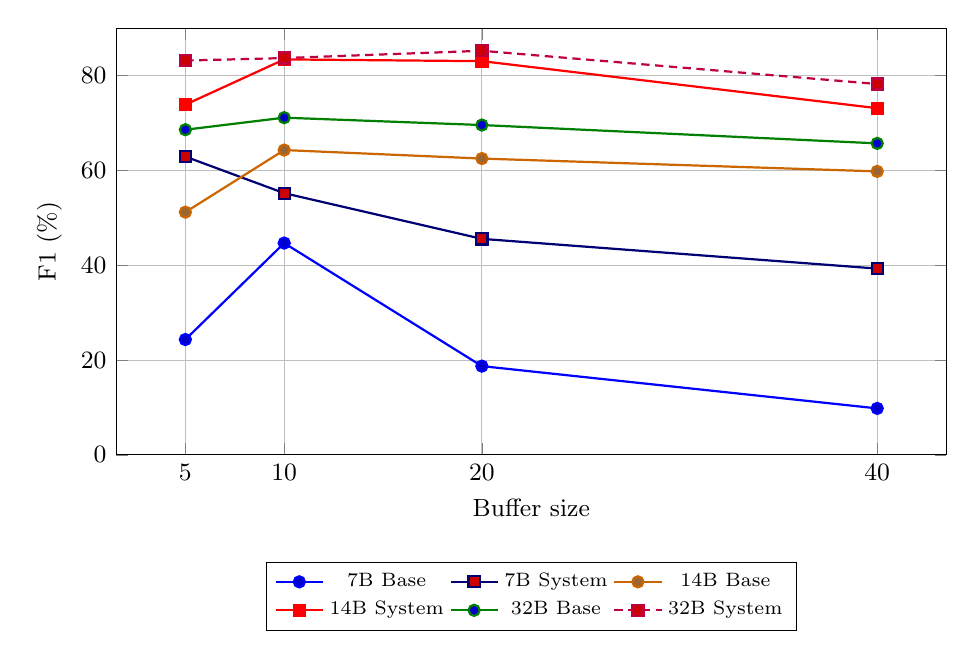
\begin{tikzpicture}
\begin{axis}[
width=\textwidth,
height=7cm,
xlabel={Buffer size},
ylabel={F1 (\%)},
xtick={5,10,20,40},
grid=both,
legend columns=3,
legend style={font=\scriptsize, at={(0.5,-0.25)}, anchor=north},
tick label style={font=\small},
label style={font=\small},
ymin=0,
ymax=90
]
\addplot+[color=blue, mark=*, thick] coordinates {(5,24.3277) (10,44.6750) (20,18.7204) (40,9.8033)};
\addlegendentry{7B Base}
\addplot+[color=blue!45!black, mark=square*, thick] coordinates {(5,62.9179) (10,55.2057) (20,45.5658) (40,39.2950)};
\addlegendentry{7B System}
\addplot+[color=orange!80!black, mark=*, thick] coordinates {(5,51.1988) (10,64.2995) (20,62.5056) (40,59.7974)};
\addlegendentry{14B Base}
\addplot+[color=red, mark=square*, thick] coordinates {(5,73.8736) (10,83.4215) (20,83.0537) (40,73.1313)};
\addlegendentry{14B System}
\addplot+[color=green!50!black, mark=*, thick] coordinates {(5,68.5899) (10,71.1312) (20,69.5766) (40,65.7086)};
\addlegendentry{32B Base}
\addplot+[color=purple, mark=square*, thick] coordinates {(5,83.1796) (10,83.7040) (20,85.2437) (40,78.2294)};
\addlegendentry{32B System}
\end{axis}
\end{tikzpicture}
\caption{Context-isolation F1 across model sizes and buffer sizes. Subchat Trees improves F1 over the linear baseline in every configuration.}
\label{fig:f1_buffer_all}
\end{figure*}

Figure~\ref{fig:pollution_buffer_all} gives the matching pollution rate. At $C=20$, pollution falls from 84.1\% to 61.5\% for 7B, for 14B it is from 39.8\% to 18.1\%, and  32.7\% to 16.5\% for 32B. This directly supports that the failure is not only forgetting, but also contamination from unrelated conversational state.

\begin{figure*}[htbp]
\centering
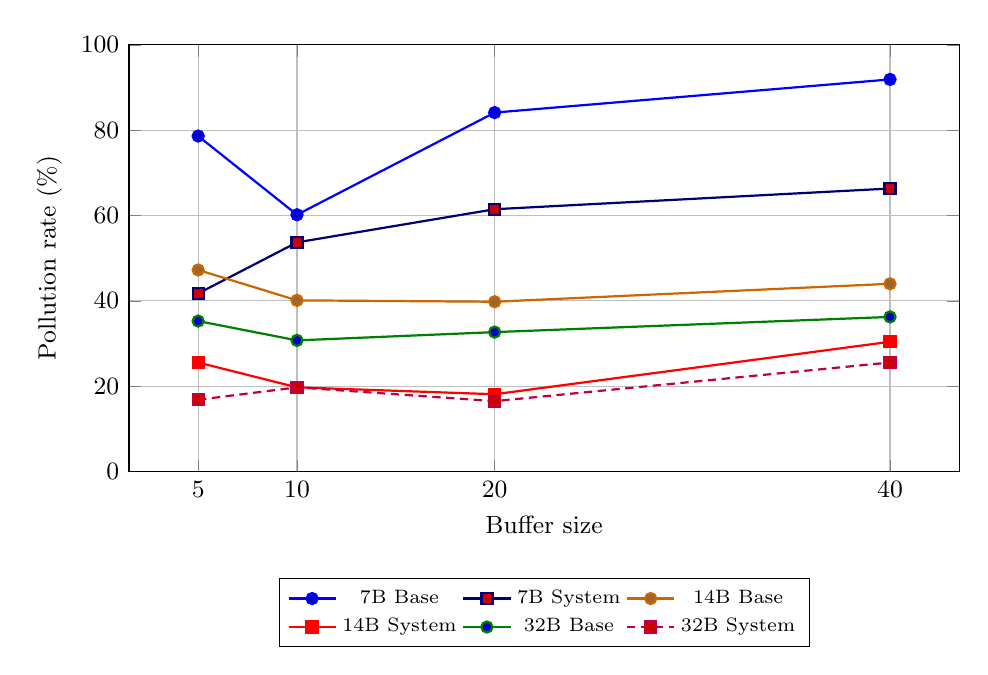
\begin{tikzpicture}
\begin{axis}[
width=\textwidth,
height=7cm,
xlabel={Buffer size},
ylabel={Pollution rate (\%)},
xtick={5,10,20,40},
grid=both,
legend columns=3,
legend style={font=\scriptsize, at={(0.5,-0.25)}, anchor=north},
tick label style={font=\small},
label style={font=\small},
ymin=0,
ymax=100
]
\addplot+[color=blue, mark=*, thick] coordinates {(5,78.6408) (10,60.1942) (20,84.1424) (40,91.9094)};
\addlegendentry{7B Base}
\addplot+[color=blue!45!black, mark=square*, thick] coordinates {(5,41.7476) (10,53.7217) (20,61.4887) (40,66.3430)};
\addlegendentry{7B System}
\addplot+[color=orange!80!black, mark=*, thick] coordinates {(5,47.2492) (10,40.1294) (20,39.8058) (40,44.0129)};
\addlegendentry{14B Base}
\addplot+[color=red, mark=square*, thick] coordinates {(5,25.5663) (10,19.7411) (20,18.1230) (40,30.4207)};
\addlegendentry{14B System}
\addplot+[color=green!50!black, mark=*, thick] coordinates {(5,35.2751) (10,30.7443) (20,32.6861) (40,36.2460)};
\addlegendentry{32B Base}
\addplot+[color=purple, mark=square*, thick] coordinates {(5,16.8285) (10,19.7411) (20,16.5049) (40,25.5663)};
\addlegendentry{32B System}
\end{axis}
\end{tikzpicture}
\caption{Pollution rate across buffer sizes. Lower values are better. Subchat Trees consistently reduces cross-topic contamination by routing turns into branch-local buffers instead of keeping all topics in one linear transcript.}
\label{fig:pollution_buffer_all}
\end{figure*}

Figure~\ref{fig:rouge1_buffer_all} summarizes the recall-probe result. The Subchat system improves average ROUGE-1 in every model-buffer setting. This matters because it shows that the tree system is preserving more topic content.

\begin{figure*}[htbp]
\centering
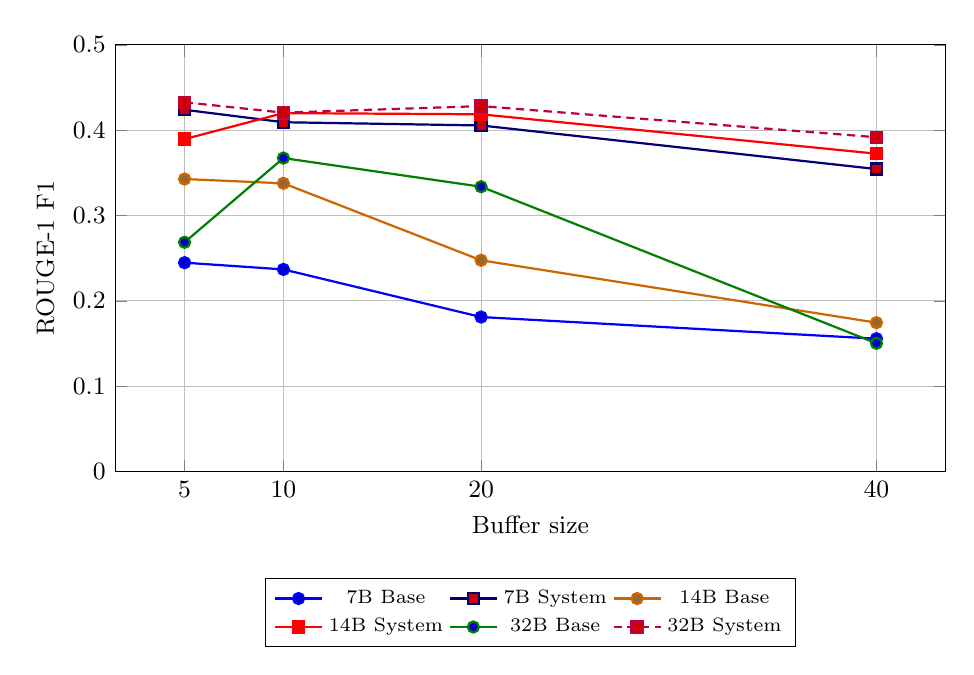
\begin{tikzpicture}
\begin{axis}[
width=\textwidth,
height=7cm,
xlabel={Buffer size},
ylabel={ROUGE-1 F1},
xtick={5,10,20,40},
grid=both,
legend columns=3,
legend style={font=\scriptsize, at={(0.5,-0.25)}, anchor=north},
tick label style={font=\small},
label style={font=\small},
ymin=0,
ymax=0.5
]
\addplot+[color=blue, mark=*, thick] coordinates {(5,0.2448) (10,0.2369) (20,0.1811) (40,0.1557)};
\addlegendentry{7B Base}
\addplot+[color=blue!45!black, mark=square*, thick] coordinates {(5,0.4240) (10,0.4094) (20,0.4056) (40,0.3545)};
\addlegendentry{7B System}
\addplot+[color=orange!80!black, mark=*, thick] coordinates {(5,0.3428) (10,0.3378) (20,0.2476) (40,0.1745)};
\addlegendentry{14B Base}
\addplot+[color=red, mark=square*, thick] coordinates {(5,0.3896) (10,0.4201) (20,0.4187) (40,0.3725)};
\addlegendentry{14B System}
\addplot+[color=green!50!black, mark=*, thick] coordinates {(5,0.2687) (10,0.3674) (20,0.3338) (40,0.1503)};
\addlegendentry{32B Base}
\addplot+[color=purple, mark=square*, thick] coordinates {(5,0.4328) (10,0.4206) (20,0.4283) (40,0.3918)};
\addlegendentry{32B System}
\end{axis}
\end{tikzpicture}
\caption{Average ROUGE-1 F1 on 43 topic-recall probes. The tree system retains more semantically relevant topic content than the linear baseline across all tested model-buffer settings.}
\label{fig:rouge1_buffer_all}
\end{figure*}

Figure~\ref{fig:probe_rag_buffer_all} focuses on recall-probe RAG decisions. Here each probe explicitly asks the model to recover prior topic content. The 14B model shows the expected pattern most clearly: baseline retrieval is high at small buffers indicating poor context retention. The Subchat System system quickly becomes buffer-sufficient. Here, 32B uses more retrieval intentionally indicating small buffer can not store complete context on a topic. As buffer size increases the retrieval rate reduces indicating better context retention in the buffer with less confusion. The model uses more retrieval when the context is unclear or insufficient, But for 7B model because its limited tool calling capability its results are irrelevant.



\begin{figure*}[htbp]
\centering
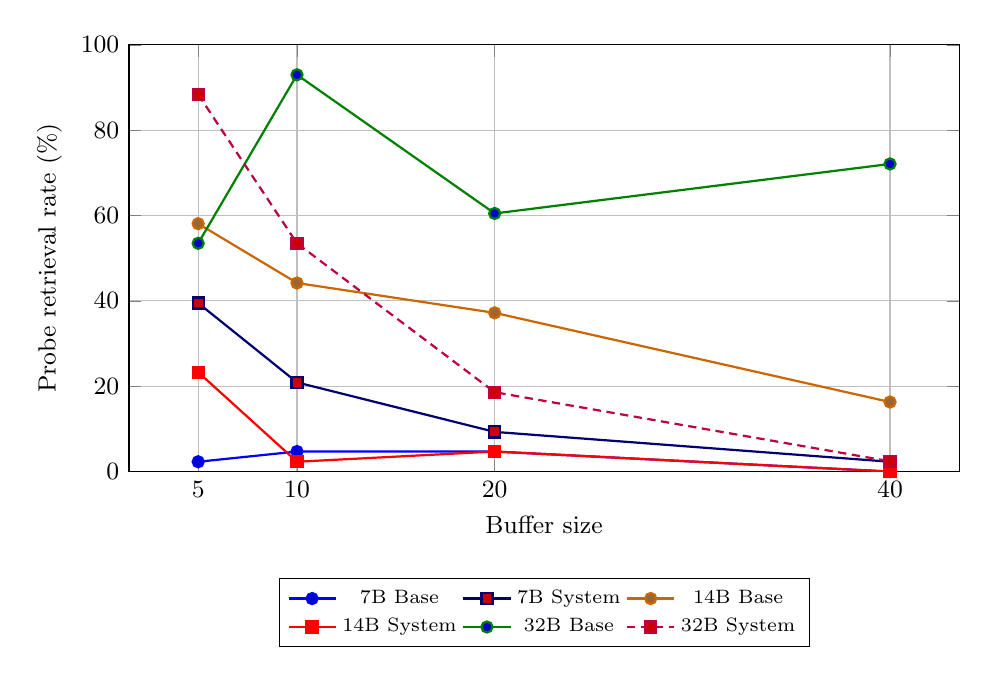
\begin{tikzpicture}
\begin{axis}[
width=\textwidth,
height=7cm,
xlabel={Buffer size},
ylabel={Probe retrieval rate (\%)},
xtick={5,10,20,40},
grid=both,
legend columns=3,
legend style={font=\scriptsize, at={(0.5,-0.25)}, anchor=north},
tick label style={font=\small},
label style={font=\small},
ymin=0,
ymax=100
]
\addplot+[color=blue, mark=*, thick] coordinates {(5,2.3) (10,4.7) (20,4.7) (40,0.0)};
\addlegendentry{7B Base}
\addplot+[color=blue!45!black, mark=square*, thick] coordinates {(5,39.5) (10,20.9) (20,9.3) (40,2.3)};
\addlegendentry{7B System}
\addplot+[color=orange!80!black, mark=*, thick] coordinates {(5,58.1) (10,44.2) (20,37.2) (40,16.3)};
\addlegendentry{14B Base}
\addplot+[color=red, mark=square*, thick] coordinates {(5,23.3) (10,2.3) (20,4.7) (40,0.0)};
\addlegendentry{14B System}
\addplot+[color=green!50!black, mark=*, thick] coordinates {(5,53.5) (10,93.0) (20,60.5) (40,72.1)};
\addlegendentry{32B Base}
\addplot+[color=purple, mark=square*, thick] coordinates {(5,88.4) (10,53.5) (20,18.6) (40,2.4)};
\addlegendentry{32B System}
\end{axis}
\end{tikzpicture}
\caption{RAG retrieval rate during the 43 recall probes. Probe retrieval is used as a memory-sufficiency signal because every probe asks the model to recover earlier topic content.}
\label{fig:probe_rag_buffer_all}
\end{figure*}

Finally, Figure~\ref{fig:tpca_buffer_all} summarizes effective token efficiency. The system sometimes uses more raw input tokens, but it uses fewer tokens per correct answer in every tested setting. This is the key correction to the initial expectation: organized context is not always shorter, but it is more detailed.

\begin{figure*}[htbp]
\centering
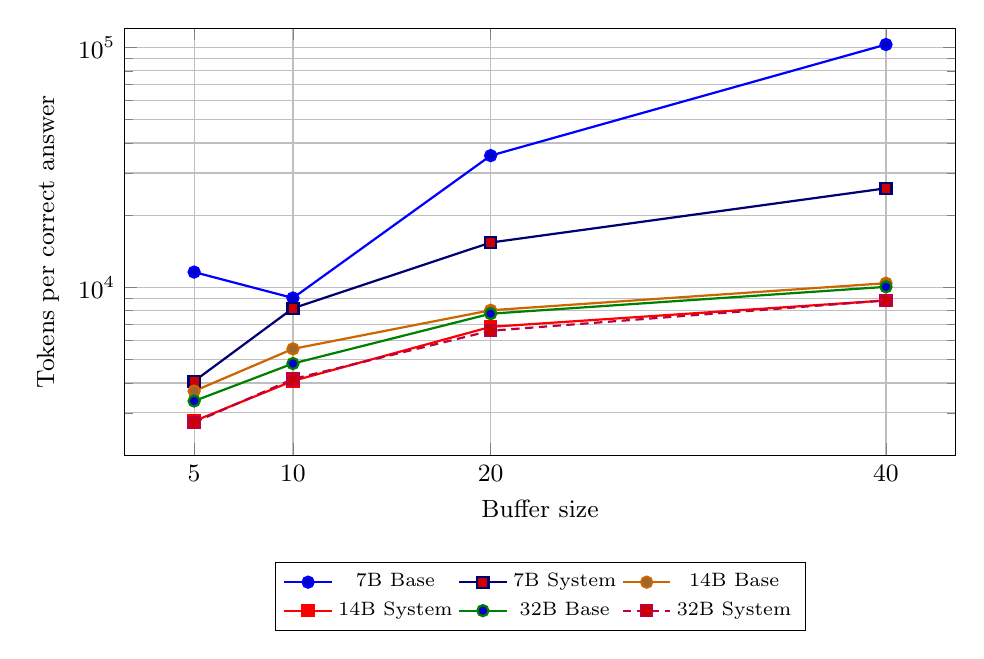
\begin{tikzpicture}
\begin{axis}[
width=\textwidth,
height=7cm,
xlabel={Buffer size},
ylabel={Tokens per correct answer},
xtick={5,10,20,40},
grid=both,
legend columns=3,
legend style={font=\scriptsize, at={(0.5,-0.25)}, anchor=north},
tick label style={font=\small},
label style={font=\small},
ymin=2000,
ymax=120000,
ymode=log
]
\addplot+[color=blue, mark=*, thick] coordinates {(5,11591.1667) (10,9038.0488) (20,35450.6531) (40,102923.4400)};
\addlegendentry{7B Base}
\addplot+[color=blue!45!black, mark=square*, thick] coordinates {(5,4067.4833) (10,8191.4196) (20,15389.0420) (40,25898.8558)};
\addlegendentry{7B System}
\addplot+[color=orange!80!black, mark=*, thick] coordinates {(5,3699.5890) (10,5547.5243) (20,8035.5215) (40,10418.1098)};
\addlegendentry{14B Base}
\addplot+[color=red, mark=square*, thick] coordinates {(5,2773.1043) (10,4079.3790) (20,6853.2095) (40,8825.9488)};
\addlegendentry{14B System}
\addplot+[color=green!50!black, mark=*, thick] coordinates {(5,3363.1150) (10,4819.4720) (20,7775.4519) (40,10059.6345)};
\addlegendentry{32B Base}
\addplot+[color=purple, mark=square*, thick] coordinates {(5,2737.7549) (10,4150.7460) (20,6600.2984) (40,8833.1696)};
\addlegendentry{32B System}
\end{axis}
\end{tikzpicture}
\caption{Tokens per correct answer across model sizes and buffer sizes. The y-axis uses a log scale because the 7B baseline becomes extremely inefficient at larger buffers.}
\label{fig:tpca_buffer_all}
\end{figure*}

\subsection{Result Summary}\label{subsec:findings_summary}

The model-specific and cross-model results support five conclusions. First, branch-local context improves topic isolation across every tested model and buffer size. Second, the useful buffer range is model-dependent: 7B is safest at short buffers, 14B works best around $C=10$ or $C=20$, and 32B peaks at $C=20$. Third, recall probes show that the tree system preserves semantic topic content even when strict prefix-following fails. Fourth, recall-probe RAG is used as the retrieval diagnostic because each probe explicitly asks for old topic content, the model uese more retrieval when context is mixed or insufficient. Fifth, raw input-token count is not the main efficiency result; tokens per correct answer shows that Subchat Trees spends computation more productively as latency for Subchat System was lower.

These results motivate conversation trees as new interface adaption. A parent conversation can hold broad context, child nodes can isolate detailed follow-ups and sibling nodes can explore alternatives without contaminating one another. This matters for ordinary chat, multi-agent workflows and embodied systems where plans, observations, corrections and subgoals naturally form nested conversational state. Long context windows increase capacity, but they do not decide which prior turns belong to the current branch. Subchat Trees makes that structure explicit.
It provides more control to the user.

\section{Discussion}\label{sec5}

\subsection{What the Results Show}\label{subsec:discussion_results}

The experiments show that conversation structure is not merely an interface preference; it changes model behavior. A linear transcript forces the LLM to infer which parts of history belong to the current turn. Subchat Trees externalizes this decision by routing turns into explicit branches. The result is lower topic pollution, higher F1, and stronger recall-probe similarity across every tested model-buffer configuration.

The cross-model pattern is also important. The 7B model shows that architecture cannot fully compensate for weak instruction following: even with better context retention, the model often fails the exact topic-prefix format. The 14B model shows the best practical balance in these runs, achieving high F1 with much lower latency than 32B. The 32B model shows the strongest absolute capability, especially at $C=20$, confirming that model scale and context architecture are complementary rather than interchangeable.

\subsection{Why Larger Buffers Are Not Always Better}\label{subsec:larger_buffers}

The buffer ablation demonstrates that more raw context can become harmful. At $C=40$, summarization is delayed and many raw turns remain in the prompt. This increases the amount of user wording, assistant wording, old instructions, possible RAG context, and unrelated topic material that the model must reconcile. The 14B and 7B models degrade noticeably at this size, and the error counts also rise. The 32B model tolerates the longer prompt better, but even it performs best at $C=20$ rather than $C=40$.

This supports a core claim of the paper: context length and context organization are different problems. Long context windows increase capacity, but they do not decide which branch of a conversation should be active. Subchat Trees improves the structure of the input before the model is asked to reason over it.

\subsection{Token Efficiency Revisited}\label{subsec:token_efficiency_revisited}

The current results revise our initial token-efficiency expectation. We expected that Subchat Trees would always reduce average input tokens because the active branch should be smaller than the full linear history. In practice, the system sometimes uses slightly more raw tokens. The logs suggest a reason: a confused baseline often answers briefly, asks for clarification, or emits a generic response, while a scoped system prompt allows the model to produce longer and more complete answers.

For this reason, tokens per correct answer is the more meaningful efficiency metric. Under that metric, Subchat Trees is consistently better. It may spend more tokens on a given turn, but it spends fewer tokens for each correct topic-tracked answer. This distinction matters for real deployment because users care about useful successful answers, not only raw prompt length.

\subsection{RAG as a Backstop Rather Than a Default}\label{subsec:rag_backstop_discussion}

The recall-probe RAG analysis suggests that retrieval works best as a backstop. In the 14B model and in larger-buffer 32B settings, the baseline frequently asks for retrieval during topic summarization because older topic details have either been evicted or mixed with unrelated turns. The tree system often decides that the branch-local buffer is already sufficient. This is the desired behavior: retrieval should be used when local context is insufficient, not as a replacement for well-organized conversation state.

The 7B exception is informative. It triggers RAG more often in the system condition, especially at short buffers, indicating that the smaller model is less reliable at judging context sufficiency. This makes the retrieval controller itself model-sensitive. Stronger models not only answer better; they also make better decisions about when memory is needed.

\subsection{Limitations}\label{subsec:limitations}

\textbf{Strict Prefix Scoring.} The deterministic scorer counts a response as incorrect if the prefix does not exactly match the expected topic. This is appropriate for testing context isolation, but it can understate semantic quality when a model answers the right content with the wrong label.

\textbf{Model Family.} The current cross-scale runs use Qwen2.5 AWQ models. Additional model families should be evaluated before claiming architecture-independent generality.

\textbf{Buffer Search.} We evaluate $C \in \{5,10,20,40\}$. The best value is model-dependent, and adaptive buffer sizing may outperform any fixed value.

\textbf{RAG Decision Reliability.} RAG decisions depend on the model's ability to judge whether local context is sufficient. The 7B results show that this controller can be miscalibrated for weaker models.

\textbf{User-Specified Branching.} The benchmark uses explicit subchat actions. Real deployments should study automatic branch suggestions and user burden.

\subsection{Deployment Considerations}\label{subsec:deployment}

Production deployment requires efficient vector-index sharding, branch archival policies, cache-aware context assembly, and safeguards for branch inheritance. The architecture is model-agnostic and can run over local vLLM backends, cloud APIs, or hybrid deployments. The main systems lesson is that the context manager should be treated as an active component of the LLM application, not a passive transcript buffer.


\section{Conclusion }\label{sec6}

Subchat Trees hierarchical conversation architecture for isolating topics in long, multi-threaded LLM dialogue. The current evaluation across Qwen2.5 7B, 14B, and 32B models shows that explicit conversation branching improves context-isolation F1 in every tested model-buffer configuration. The best absolute result is obtained by the 32B model at $C=20$, where F1 rises from 69.6\% to 85.2\% and pollution falls from 32.7\% to 16.5\%. The 14B model reaches a similar system F1 of 83.4\% at $C=10$ and 83.1\% at $C=20$, making it the strongest practical tradeoff in these runs.

The recall probes add a second conclusion: Subchat Trees preserves semantically relevant topic content, not only topic labels. Across all models and buffers, system ROUGE-1 exceeds the baseline. Finally, the efficiency analysis shows that raw input-token count is not sufficient for evaluating context architectures. The system sometimes produces longer prompts or completions, but it consistently reduces tokens per correct answer.

Overall, the results support the paper's central claim: long conversations need structure user centric control, not only longer context window. This can significantly imporve performance in multi-tasking system where a user or agent can inherit from a parent node edit in its own sub-node with parallel execution.

% \subsection{Future Directions}\label{subsec:future}

% \textbf{Adaptive Memory Management.} Learn optimal buffer sizes and eviction policies per topic through reinforcement learning.

% \textbf{Automatic Subchat Suggestion.} Use topic-shift classifiers to detect context drift and suggest subchat creation proactively.

% \textbf{Cross-Node Synthesis.} Controlled mechanisms to merge insights from multiple branches while preserving per-branch isolation guarantees.

% \textbf{Multi-Modal Extension.} Apply hierarchical structuring to conversations involving images, code, and documents.

% \textbf{Human Studies.} Conduct user studies comparing Subchat Trees to linear chat on real-world tasks (research, coding, creative writing) to measure cognitive load and task completion.

% \textbf{Alternative Backends.} Evaluate with GPT-4, Claude, and additional open-source models to assess generalizability across LLM families.

% \textbf{Graph Extensions.} Allow directed acyclic graph (DAG) structures where nodes have multiple parents for complex information synthesis.

\subsection{Impact}\label{subsec:impact}

Subchat Trees addresses critical challenges in conversational AI:
\begin{itemize}
    \item \textbf{Privacy:} Isolated contexts prevent sensitive information leakage across topics.
    \item \textbf{Accuracy:} Reduced pollution improves reliability in high-stakes domains (medicine, law, finance).
    \item \textbf{Cost:} Token efficiency reduces barriers for resource-constrained users and organizations.
    \item \textbf{Accessibility:} Explicit conversation structure aids users in navigating complex, multi-topic discussions.
\end{itemize}

We release our implementation, scenario datasets, and evaluation framework as open-source software to accelerate research in structured conversational AI.

%%==================================%%
%% BACK MATTER                     %%
%%==================================%%

\bmhead{Supplementary Information}

The complete source code for Subchat Trees is available at our GitHub repository, including the FastAPI backend, Next.js frontend, final VBRI dataset (JSON format), Kaggle evaluation notebook, evaluation scripts, and buffer-wise result bundles across four buffer sizes.

\bmhead{Acknowledgements}

We thank the developers of ChromaDB, SentenceTransformers, and the Llama and Qwen model families for providing the foundational tools that enabled this research. We also acknowledge the LMSYS team for releasing the Chat-1M dataset~\cite{zheng2024lmsyschat}, the Groq team for API access and the Kaggle platform for GPU compute resources.

\backmatter

\section*{Declarations}

\begin{itemize}
\item \textbf{Funding:} Not applicable.
\item \textbf{Conflict of interest:} The authors declare no competing interests.
\item \textbf{Ethics approval:} Not applicable.
\item \textbf{Consent to participate:} Not applicable.
\item \textbf{Consent for publication:} Not applicable.
\item \textbf{Data availability:} Test scenarios and evaluation logs are available in the supplementary materials. The LMSYS-Chat-1M dataset~\cite{zheng2024lmsyschat} is publicly available.
\item \textbf{Code availability:} Source code is available at: \url{https://github.com/moonmehedi/Subchat-Trees-A-Scalable-Architecture-for-Multi-Threaded-Dialogue-and-Context-Isolation-in-LLM}
\item \textbf{Author contribution:} All authors contributed to the design, implementation, and evaluation of the system. All authors reviewed and approved the final manuscript.
\end{itemize}

\begin{appendices}

\section{Source Conversation Details}\label{secA1}

The five LMSYS-derived source conversations used to construct the final VBRI dataset are briefly described below.

\textbf{\texttt{22807e655dd042348cb0ee4023672e70}.} Tests persona isolation (old man, newlywed, physicist, dog), a Twenty Questions game with repeated role-reversal failures, and LLM meta-discussion. The critical test is whether the model can maintain game state when roles are explicitly swapped.

\textbf{\texttt{6c4992f0aed04dd3bf9a4bc225bb4fb0}.} Tests containment of a failure mode where the model enters a 15+ iteration repetitive loop (``I am able to process and analyze large amounts of text data...''), alongside medical treatments, electroculture, AI consciousness, literature, and pandemic-safety topics.

\textbf{\texttt{8d10c143f8fc4a7599a5a18778fec112}.} The broadest source conversation, covering DSP/wavelets, C code, medical genetics (DSD, Klinefelter syndrome), Linux audio, statistics, quantum physics, cosmology, music physics, sci-fi (Liu Cixin), space exploration, Belgium geography, HAL-9000 roleplay, and games.

\textbf{\texttt{eaf06f12a1d74e5ca30a7ca94a7c4128}.} Tests isolation of an argumentative failure mode where the model incorrectly halves 1\,tsp vanilla to 1/4\,tsp (should be 1/2\,tsp) and defends the error across multiple turns, with interleaved jokes, cookie preferences, and an emoji guessing game.

\textbf{\texttt{ec366fd3e4b5482e8acac750f9b3b55b}.} Includes repeated user-requested context resets across topics spanning Indian history, logic puzzles, LSAT reasoning, Indian legal code, child nutrition, astrology, elections, Bhutan travel, recipes, therapy, and chess.

\textbf{\texttt{merged\_vbri\_temporal}.} The final benchmark merges the five source conversations into a single 309-turn conversation using the VBRI algorithm described in Section~\ref{subsubsec:dataset}. It spans 59 distinct topics and contains 91 topic switches, 64 source-conversation switches, and 25 topic returns. This scenario serves as the testbed for both topic-prefix isolation and recall-probe evaluation.

\section{Kaggle Notebook Execution Pipeline}\label{secA2}

The evaluation pipeline is packaged as a self-contained Kaggle notebook (\texttt{kaggle\_test\_runner.ipynb}) with the following cells:

\begin{enumerate}
    \item \textbf{Cell~1:} Install vLLM dependencies (\texttt{vllm}, \texttt{triton}).
    \item \textbf{Cell~2:} Import libraries and verify GPU availability.
    \item \textbf{Cell~3:} Load Kaggle secrets (GitHub token, Groq key, HuggingFace token) and set \texttt{LLM\_BACKEND=vllm}.
    \item \textbf{Cell~4:} Load Qwen-2.5 14B AWQ with \texttt{vllm.LLM()}, 4-bit quantization, 91\% GPU memory utilization, and \texttt{max\_model\_len=5000}.
    \item \textbf{Cell~5:} Clone the repository (\texttt{kaggle-run} branch) and pull scenario files from Git LFS.
    \item \textbf{Cell~6:} Register the vLLM model with the backend via \texttt{VLLMClient.set\_model(llm)}.
    \item \textbf{Cell~7:} Install backend Python requirements.
    \item \textbf{Cell~8:} Quick integration test (create node, send message, verify response).
    \item \textbf{Cell~9:} Execute the configured serverless evaluation: validate scenario JSON files, run baseline and system tests for the selected buffer sizes, generate Markdown tables, raw JSON metrics, recall-probe logs, and buffer-specific component logs.
\end{enumerate}

The notebook version used for the final benchmark targets \texttt{merged\_realistic\_interleaved.json}; the current result section reports the completed 7B, 14B, and 32B runs for buffer sizes $C \in \{5,10,20,40\}$.

\section{Per-Topic Confusion Matrix Methodology}\label{secA3}

Rather than computing a single global confusion matrix, we compute per-topic matrices. For each of the 59 topics $\tau_i$, we count:
\begin{itemize}
    \item $\text{TP}_i$: Responses correctly scored as belonging to $\tau_i$.
    \item $\text{FP}_i$: Responses incorrectly attributed to $\tau_i$ when the ground truth is a different topic.
    \item $\text{FN}_i$: Responses where $\tau_i$ was expected but a different topic was returned.
\end{itemize}

The weighted-average metrics reported in the model-specific context-isolation tables (Tables~\ref{tab:7b_context_main}, \ref{tab:14b_context_main}, and~\ref{tab:32b_context_main}) weight each topic's precision, recall, and F1 by its support (number of ground-truth instances), ensuring that topics with more test steps contribute proportionally to the aggregate. Macro-average metrics treat all topics equally regardless of support.


\section{Complete Merged Result Tables}\label{secA4}

This appendix reproduces the complete merged tables generated from the current result folders for 7B, 14B, and 32B models across buffer sizes $C \in \{5,10,20,40\}$.

\subsection{7B Merged Tables}\label{app:7b_merged}
\begin{landscape}
\tiny
\begin{longtable}{@{}p{3.8cm}cccccccc@{}}
\caption{7B: merged context-isolation metrics.}\label{tab:app_7b_context}\\

\toprule
\textbf{Metric} & \multicolumn{2}{c}{\textbf{Buffer 5}} & \multicolumn{2}{c}{\textbf{Buffer 10}} & \multicolumn{2}{c}{\textbf{Buffer 20}} & \multicolumn{2}{c}{\textbf{Buffer 40}} \\
\cmidrule(lr){2-3}\cmidrule(lr){4-5}\cmidrule(lr){6-7}\cmidrule(lr){8-9}
 & \textbf{Base} & \textbf{System} & \textbf{Base} & \textbf{System} & \textbf{Base} & \textbf{System} & \textbf{Base} & \textbf{System} \\
\midrule
\endfirsthead

\toprule
\textbf{Metric} & \multicolumn{2}{c}{\textbf{Buffer 5}} & \multicolumn{2}{c}{\textbf{Buffer 10}} & \multicolumn{2}{c}{\textbf{Buffer 20}} & \multicolumn{2}{c}{\textbf{Buffer 40}} \\
\cmidrule(lr){2-3}\cmidrule(lr){4-5}\cmidrule(lr){6-7}\cmidrule(lr){8-9}
 & \textbf{Base} & \textbf{System} & \textbf{Base} & \textbf{System} & \textbf{Base} & \textbf{System} & \textbf{Base} & \textbf{System} \\
\midrule
\endhead
Precision & 44.7\% & 84.0\% & 71.5\% & 88.7\% & 34.9\% & 80.7\% & 21.5\% & 76.2\% \\
Recall & 21.1\% & 58.1\% & 39.6\% & 46.1\% & 15.6\% & 38.3\% & 7.8\% & 33.4\% \\
F1 & 24.3\% & 62.9\% & 44.7\% & 55.2\% & 18.7\% & 45.6\% & 9.8\% & 39.3\% \\
Accuracy & 21.4\% & 58.3\% & 39.8\% & 46.3\% & 15.9\% & 38.5\% & 8.1\% & 33.7\% \\
Pollution Rate & 78.6\% & 41.7\% & 60.2\% & 53.7\% & 84.1\% & 61.5\% & 91.9\% & 66.3\% \\
Macro Precision & 48.5\% & 74.4\% & 70.9\% & 85.6\% & 41.7\% & 76.0\% & 29.0\% & 72.8\% \\
Macro Recall & 33.7\% & 59.6\% & 49.4\% & 59.7\% & 24.7\% & 50.5\% & 17.8\% & 41.4\% \\
Macro F1 & 35.2\% & 60.8\% & 53.6\% & 65.3\% & 27.2\% & 55.6\% & 19.0\% & 46.5\% \\
\botrule
\end{longtable}
\normalsize
\end{landscape}
\begin{landscape}
\tiny
\begin{longtable}{@{}p{3.8cm}cccccccc@{}}
\caption{7B: merged aggregate recall scores and probe cost.}\label{tab:app_7b_recall_agg}\\

\toprule
\textbf{Metric} & \multicolumn{2}{c}{\textbf{Buffer 5}} & \multicolumn{2}{c}{\textbf{Buffer 10}} & \multicolumn{2}{c}{\textbf{Buffer 20}} & \multicolumn{2}{c}{\textbf{Buffer 40}} \\
\cmidrule(lr){2-3}\cmidrule(lr){4-5}\cmidrule(lr){6-7}\cmidrule(lr){8-9}
 & \textbf{Base} & \textbf{System} & \textbf{Base} & \textbf{System} & \textbf{Base} & \textbf{System} & \textbf{Base} & \textbf{System} \\
\midrule
\endfirsthead

\toprule
\textbf{Metric} & \multicolumn{2}{c}{\textbf{Buffer 5}} & \multicolumn{2}{c}{\textbf{Buffer 10}} & \multicolumn{2}{c}{\textbf{Buffer 20}} & \multicolumn{2}{c}{\textbf{Buffer 40}} \\
\cmidrule(lr){2-3}\cmidrule(lr){4-5}\cmidrule(lr){6-7}\cmidrule(lr){8-9}
 & \textbf{Base} & \textbf{System} & \textbf{Base} & \textbf{System} & \textbf{Base} & \textbf{System} & \textbf{Base} & \textbf{System} \\
\midrule
\endhead
Avg ROUGE-1 (F1) & 0.2448 & 0.4240 & 0.2369 & 0.4094 & 0.1811 & 0.4056 & 0.1557 & 0.3545 \\
Avg ROUGE-L (F1) & 0.1270 & 0.3004 & 0.1349 & 0.3097 & 0.1016 & 0.3194 & 0.0861 & 0.2574 \\
Avg BLEU-2 & 0.0364 & 0.1581 & 0.0324 & 0.1259 & 0.0205 & 0.1325 & 0.0172 & 0.1142 \\
Topics Probed & 43 & 43 & 43 & 43 & 43 & 43 & 43 & 43 \\
Total Probe Tokens & 158,043 & 121,521 & 252,519 & 188,722 & 336,942 & 284,817 & 472,634 & 403,852 \\
Avg Tokens per Probe & 3,675 & 2,826 & 5,873 & 4,389 & 7,836 & 6,624 & 10,991 & 9,392 \\
Total Probe Latency & 918.00s & 710.28s & 814.85s & 776.91s & 767.61s & 792.74s & 723.47s & 703.08s \\
Avg Probe Latency & 21.35s & 16.52s & 18.95s & 18.07s & 17.85s & 18.44s & 16.82s & 16.35s \\
\botrule
\end{longtable}
\normalsize
\end{landscape}
\begin{landscape}
\tiny
\begin{longtable}{@{}p{3.8cm}cccccccc@{}}
\caption{7B: per-topic ROUGE-1 F1 across buffers.}\label{tab:app_7b_rouge1_topics}\\

\toprule
\textbf{Metric} & \multicolumn{2}{c}{\textbf{Buffer 5}} & \multicolumn{2}{c}{\textbf{Buffer 10}} & \multicolumn{2}{c}{\textbf{Buffer 20}} & \multicolumn{2}{c}{\textbf{Buffer 40}} \\
\cmidrule(lr){2-3}\cmidrule(lr){4-5}\cmidrule(lr){6-7}\cmidrule(lr){8-9}
 & \textbf{Base} & \textbf{System} & \textbf{Base} & \textbf{System} & \textbf{Base} & \textbf{System} & \textbf{Base} & \textbf{System} \\
\midrule
\endfirsthead

\toprule
\textbf{Metric} & \multicolumn{2}{c}{\textbf{Buffer 5}} & \multicolumn{2}{c}{\textbf{Buffer 10}} & \multicolumn{2}{c}{\textbf{Buffer 20}} & \multicolumn{2}{c}{\textbf{Buffer 40}} \\
\cmidrule(lr){2-3}\cmidrule(lr){4-5}\cmidrule(lr){6-7}\cmidrule(lr){8-9}
 & \textbf{Base} & \textbf{System} & \textbf{Base} & \textbf{System} & \textbf{Base} & \textbf{System} & \textbf{Base} & \textbf{System} \\
\midrule
\endhead
ai\_chat\_tools & 0.2021 & 0.4254 & 0.2410 & 0.2101 & 0.1660 & 0.2949 & 0.1821 & 0.2635 \\
ai\_consciousness & 0.2580 & 0.4540 & 0.1501 & 0.2671 & 0.1476 & 0.2366 & 0.1662 & 0.3648 \\
ai\_consciousness\_friendship & 0.3911 & 0.4905 & 0.2495 & 0.4639 & 0.2624 & 0.4216 & 0.3581 & 0.5567 \\
ai\_meta & 0.2663 & 0.2581 & 0.2994 & 0.3636 & 0.1513 & 0.2757 & 0.1769 & 0.3214 \\
bhutan\_travel & 0.2285 & 0.4050 & 0.1547 & 0.4433 & 0.3182 & 0.0975 & 0.3304 & 0.5440 \\
chess & 0.3337 & 0.3140 & 0.1864 & 0.5036 & 0.2256 & 0.3418 & 0.2354 & 0.4324 \\
child\_nutrition & 0.1623 & 0.3047 & 0.2113 & 0.2341 & 0.1610 & 0.2655 & 0.1934 & 0.1596 \\
cookies\_recipe\_halving & 0.3874 & 0.8199 & 0.4431 & 0.5997 & 0.2359 & 0.6293 & 0.0841 & 0.6293 \\
cookies\_recipe\_halving\_argument & 0.4291 & 0.5270 & 0.3927 & 0.4427 & 0.2213 & 0.6188 & 0.2921 & 0.6237 \\
cookies\_recipe\_halving\_corrections & 0.3542 & 0.5931 & 0.3301 & 0.6345 & 0.0661 & 0.6736 & 0.1684 & 0.6911 \\
cookies\_recipe\_halving\_math\_errors & 0.3121 & 0.8059 & 0.4259 & 0.6610 & 0.0911 & 0.6458 & 0.2279 & 0.6458 \\
covid\_safety & 0.3567 & 0.3862 & 0.2496 & 0.3871 & 0.2354 & 0.0880 & 0.1893 & 0.0698 \\
covid\_safety\_hiv\_aids & 0.1604 & 0.3547 & 0.2304 & 0.1854 & 0.1710 & 0.3229 & 0.0599 & 0.1566 \\
dsp\_wavelets & 0.1245 & 0.1577 & 0.1007 & 0.1582 & 0.1588 & 0.1950 & 0.0609 & 0.0963 \\
electroculture & 0.0892 & 0.2333 & 0.1120 & 0.2422 & 0.0149 & 0.3496 & 0.0591 & 0.3274 \\
emoji\_game & 0.1515 & 0.1117 & 0.1811 & 0.2156 & 0.2063 & 0.3143 & 0.0419 & 0.3000 \\
game\_degree\_guess & 0.1891 & 0.4330 & 0.2290 & 0.5918 & 0.2200 & 0.6593 & 0.1073 & 0.4763 \\
game\_twenty\_questions & 0.1354 & 0.1918 & 0.2139 & 0.2957 & 0.1749 & 0.4551 & 0.0499 & 0.3575 \\
geography\_belgium & 0.3109 & 0.6798 & 0.3982 & 0.5222 & 0.4461 & 0.4358 & 0.1328 & 0.6110 \\
humanity\_future\_150y & 0.3412 & 0.4418 & 0.2256 & 0.4732 & 0.1368 & 0.4710 & 0.0458 & 0.4304 \\
indian\_astrology & 0.1591 & 0.3579 & 0.1761 & 0.2527 & 0.0289 & 0.2203 & 0.0424 & 0.0185 \\
indian\_history & 0.1420 & 0.6154 & 0.1211 & 0.5679 & 0.1869 & 0.6870 & 0.1618 & 0.5185 \\
indian\_legal & 0.2342 & 0.6822 & 0.2560 & 0.4519 & 0.2108 & 0.3882 & 0.2389 & 0.3860 \\
indian\_legal\_family & 0.1410 & 0.3434 & 0.2133 & 0.4432 & 0.2343 & 0.6025 & 0.1953 & 0.0270 \\
jokes & 0.3048 & 0.6551 & 0.1566 & 0.6627 & 0.1901 & 0.5973 & 0.2804 & 0.6638 \\
karnataka\_elections & 0.2515 & 0.3884 & 0.3563 & 0.7264 & 0.0278 & 0.3956 & 0.2916 & 0.2995 \\
linux\_audio & 0.3791 & 0.4970 & 0.3067 & 0.5253 & 0.2950 & 0.4704 & 0.3300 & 0.0591 \\
literature\_camus & 0.2144 & 0.3049 & 0.1960 & 0.2961 & 0.1765 & 0.3049 & 0.2126 & 0.0270 \\
llm\_knowledge & 0.3093 & 0.2710 & 0.2396 & 0.3205 & 0.1585 & 0.2670 & 0.0194 & 0.2085 \\
logic\_puzzle & 0.2775 & 0.7113 & 0.0833 & 0.6097 & 0.2430 & 0.4903 & 0.1870 & 0.6263 \\
lsat\_medical\_conference & 0.1429 & 0.7286 & 0.1687 & 0.4985 & 0.0938 & 0.6478 & 0.1206 & 0.6977 \\
lsat\_product\_codes & 0.1284 & 0.2628 & 0.1806 & 0.2555 & 0.0268 & 0.1056 & 0.0762 & 0.2708 \\
medical\_dsd & 0.2218 & 0.6041 & 0.1549 & 0.3869 & 0.2271 & 0.3125 & 0.1974 & 0.3406 \\
personas\_roleplay & 0.2727 & 0.4322 & 0.2299 & 0.4697 & 0.2337 & 0.7983 & 0.0653 & 0.4448 \\
physics\_cosmology & 0.3249 & 0.6305 & 0.3117 & 0.4609 & 0.2785 & 0.0990 & 0.2125 & 0.4503 \\
physics\_violin\_nanoscale & 0.3377 & 0.1142 & 0.3416 & 0.3005 & 0.2473 & 0.4119 & 0.1557 & 0.2977 \\
scifi\_films & 0.2909 & 0.2210 & 0.2248 & 0.2548 & 0.0148 & 0.1974 & 0.0601 & 0.2759 \\
scifi\_films\_hal9000 & 0.1155 & 0.3492 & 0.2967 & 0.3358 & 0.2331 & 0.4793 & 0.0791 & 0.4857 \\
scifi\_films\_hal9000\_games & 0.1543 & 0.3055 & 0.2009 & 0.2618 & 0.1588 & 0.3373 & 0.0462 & 0.2645 \\
scifi\_films\_liu\_cixin & 0.2654 & 0.2099 & 0.2943 & 0.3290 & 0.3026 & 0.4444 & 0.0996 & 0.3695 \\
therapy & 0.2608 & 0.3848 & 0.2003 & 0.4561 & 0.3206 & 0.5734 & 0.1086 & 0.0428 \\
therapy\_manipulation & 0.2090 & 0.3110 & 0.1898 & 0.4475 & 0.0466 & 0.4167 & 0.0984 & 0.0867 \\
wildfires\_alberta & 0.2067 & 0.4619 & 0.2640 & 0.3957 & 0.0396 & 0.4011 & 0.2525 & 0.3232 \\
\botrule
\end{longtable}
\normalsize
\end{landscape}
\begin{landscape}
\tiny
\begin{longtable}{@{}p{3.8cm}cccccccc@{}}
\caption{7B: per-topic ROUGE-L F1 across buffers.}\label{tab:app_7b_rougel_topics}\\

\toprule
\textbf{Metric} & \multicolumn{2}{c}{\textbf{Buffer 5}} & \multicolumn{2}{c}{\textbf{Buffer 10}} & \multicolumn{2}{c}{\textbf{Buffer 20}} & \multicolumn{2}{c}{\textbf{Buffer 40}} \\
\cmidrule(lr){2-3}\cmidrule(lr){4-5}\cmidrule(lr){6-7}\cmidrule(lr){8-9}
 & \textbf{Base} & \textbf{System} & \textbf{Base} & \textbf{System} & \textbf{Base} & \textbf{System} & \textbf{Base} & \textbf{System} \\
\midrule
\endfirsthead

\toprule
\textbf{Metric} & \multicolumn{2}{c}{\textbf{Buffer 5}} & \multicolumn{2}{c}{\textbf{Buffer 10}} & \multicolumn{2}{c}{\textbf{Buffer 20}} & \multicolumn{2}{c}{\textbf{Buffer 40}} \\
\cmidrule(lr){2-3}\cmidrule(lr){4-5}\cmidrule(lr){6-7}\cmidrule(lr){8-9}
 & \textbf{Base} & \textbf{System} & \textbf{Base} & \textbf{System} & \textbf{Base} & \textbf{System} & \textbf{Base} & \textbf{System} \\
\midrule
\endhead
ai\_chat\_tools & 0.1276 & 0.2810 & 0.1480 & 0.0922 & 0.0779 & 0.1909 & 0.0802 & 0.1579 \\
ai\_consciousness & 0.1159 & 0.1982 & 0.0746 & 0.1786 & 0.0779 & 0.1840 & 0.0803 & 0.3455 \\
ai\_consciousness\_friendship & 0.1508 & 0.2503 & 0.1083 & 0.3138 & 0.1239 & 0.3253 & 0.1266 & 0.3264 \\
ai\_meta & 0.1241 & 0.1263 & 0.1465 & 0.2466 & 0.0798 & 0.1892 & 0.0750 & 0.1923 \\
bhutan\_travel & 0.1183 & 0.3870 & 0.0889 & 0.3488 & 0.3094 & 0.0796 & 0.1550 & 0.4456 \\
chess & 0.1423 & 0.1433 & 0.0993 & 0.4331 & 0.0986 & 0.2852 & 0.1111 & 0.3430 \\
child\_nutrition & 0.0724 & 0.1439 & 0.0999 & 0.1448 & 0.0744 & 0.2157 & 0.0889 & 0.1138 \\
cookies\_recipe\_halving & 0.1635 & 0.7291 & 0.3096 & 0.4749 & 0.1303 & 0.4829 & 0.0664 & 0.4829 \\
cookies\_recipe\_halving\_argument & 0.2162 & 0.3556 & 0.2024 & 0.2710 & 0.1270 & 0.4094 & 0.1445 & 0.3041 \\
cookies\_recipe\_halving\_corrections & 0.1644 & 0.3690 & 0.2300 & 0.4655 & 0.0555 & 0.3473 & 0.1006 & 0.3740 \\
cookies\_recipe\_halving\_math\_errors & 0.1545 & 0.6430 & 0.2630 & 0.5428 & 0.0771 & 0.5432 & 0.1348 & 0.5432 \\
covid\_safety & 0.1783 & 0.1501 & 0.1110 & 0.2979 & 0.1050 & 0.0773 & 0.0930 & 0.0640 \\
covid\_safety\_hiv\_aids & 0.0702 & 0.2993 & 0.1130 & 0.1440 & 0.0895 & 0.3091 & 0.0434 & 0.1398 \\
dsp\_wavelets & 0.0728 & 0.0791 & 0.0597 & 0.0910 & 0.0812 & 0.1269 & 0.0359 & 0.0713 \\
electroculture & 0.0635 & 0.2119 & 0.0744 & 0.2382 & 0.0100 & 0.3391 & 0.0456 & 0.3265 \\
emoji\_game & 0.1038 & 0.0806 & 0.1274 & 0.1540 & 0.1375 & 0.2738 & 0.0389 & 0.1529 \\
game\_degree\_guess & 0.1006 & 0.2108 & 0.1279 & 0.4014 & 0.1087 & 0.5149 & 0.0683 & 0.3312 \\
game\_twenty\_questions & 0.0771 & 0.1120 & 0.1262 & 0.1632 & 0.0885 & 0.3913 & 0.0369 & 0.3238 \\
geography\_belgium & 0.1329 & 0.5853 & 0.1663 & 0.4182 & 0.2032 & 0.4071 & 0.0945 & 0.3808 \\
humanity\_future\_150y & 0.2547 & 0.3886 & 0.1213 & 0.4630 & 0.0815 & 0.4684 & 0.0316 & 0.4094 \\
indian\_astrology & 0.0829 & 0.2640 & 0.0999 & 0.2097 & 0.0246 & 0.1735 & 0.0306 & 0.0139 \\
indian\_history & 0.0966 & 0.4497 & 0.0895 & 0.3580 & 0.1121 & 0.4609 & 0.1225 & 0.4233 \\
indian\_legal & 0.1155 & 0.6173 & 0.1351 & 0.4182 & 0.1197 & 0.3173 & 0.1194 & 0.2202 \\
indian\_legal\_family & 0.0832 & 0.2144 & 0.1343 & 0.3735 & 0.1179 & 0.5665 & 0.1316 & 0.0180 \\
jokes & 0.1628 & 0.5226 & 0.1325 & 0.6209 & 0.1281 & 0.4887 & 0.1771 & 0.5319 \\
karnataka\_elections & 0.1304 & 0.2810 & 0.1987 & 0.6430 & 0.0199 & 0.2706 & 0.1434 & 0.2047 \\
linux\_audio & 0.1954 & 0.3550 & 0.1488 & 0.2373 & 0.1605 & 0.2391 & 0.1449 & 0.0432 \\
literature\_camus & 0.1067 & 0.2587 & 0.0993 & 0.2663 & 0.0858 & 0.2018 & 0.0937 & 0.0240 \\
llm\_knowledge & 0.1494 & 0.1492 & 0.1125 & 0.1700 & 0.0784 & 0.2137 & 0.0141 & 0.1513 \\
logic\_puzzle & 0.1659 & 0.5798 & 0.0702 & 0.5306 & 0.1371 & 0.3666 & 0.1220 & 0.4811 \\
lsat\_medical\_conference & 0.0772 & 0.5771 & 0.1139 & 0.4758 & 0.0704 & 0.6337 & 0.0778 & 0.6487 \\
lsat\_product\_codes & 0.0840 & 0.2416 & 0.1213 & 0.2247 & 0.0255 & 0.1035 & 0.0557 & 0.2610 \\
medical\_dsd & 0.0988 & 0.3196 & 0.0896 & 0.2373 & 0.0939 & 0.2199 & 0.1138 & 0.1339 \\
personas\_roleplay & 0.1096 & 0.1648 & 0.1236 & 0.3371 & 0.1116 & 0.7344 & 0.0435 & 0.2517 \\
physics\_cosmology & 0.1861 & 0.4972 & 0.2315 & 0.2868 & 0.2089 & 0.0921 & 0.1324 & 0.3874 \\
physics\_violin\_nanoscale & 0.1876 & 0.0913 & 0.2067 & 0.1897 & 0.1649 & 0.2348 & 0.1107 & 0.2558 \\
scifi\_films & 0.1211 & 0.1099 & 0.1172 & 0.1471 & 0.0121 & 0.1268 & 0.0384 & 0.2287 \\
scifi\_films\_hal9000 & 0.0878 & 0.1637 & 0.1540 & 0.1810 & 0.1084 & 0.4247 & 0.0494 & 0.2491 \\
scifi\_films\_hal9000\_games & 0.0874 & 0.1468 & 0.1112 & 0.1527 & 0.0907 & 0.2099 & 0.0361 & 0.1391 \\
scifi\_films\_liu\_cixin & 0.1503 & 0.1125 & 0.1625 & 0.2857 & 0.1655 & 0.3670 & 0.0630 & 0.2516 \\
therapy & 0.1365 & 0.3266 & 0.1202 & 0.3894 & 0.1283 & 0.4230 & 0.0658 & 0.0293 \\
therapy\_manipulation & 0.1061 & 0.2736 & 0.1005 & 0.3151 & 0.0361 & 0.3913 & 0.0679 & 0.0559 \\
wildfires\_alberta & 0.1348 & 0.4571 & 0.1305 & 0.3828 & 0.0321 & 0.3140 & 0.0957 & 0.2352 \\
\botrule
\end{longtable}
\normalsize
\end{landscape}
\begin{landscape}
\tiny
\begin{longtable}{@{}p{3.8cm}cccccccc@{}}
\caption{7B: per-topic BLEU-2 across buffers.}\label{tab:app_7b_bleu_topics}\\

\toprule
\textbf{Metric} & \multicolumn{2}{c}{\textbf{Buffer 5}} & \multicolumn{2}{c}{\textbf{Buffer 10}} & \multicolumn{2}{c}{\textbf{Buffer 20}} & \multicolumn{2}{c}{\textbf{Buffer 40}} \\
\cmidrule(lr){2-3}\cmidrule(lr){4-5}\cmidrule(lr){6-7}\cmidrule(lr){8-9}
 & \textbf{Base} & \textbf{System} & \textbf{Base} & \textbf{System} & \textbf{Base} & \textbf{System} & \textbf{Base} & \textbf{System} \\
\midrule
\endfirsthead

\toprule
\textbf{Metric} & \multicolumn{2}{c}{\textbf{Buffer 5}} & \multicolumn{2}{c}{\textbf{Buffer 10}} & \multicolumn{2}{c}{\textbf{Buffer 20}} & \multicolumn{2}{c}{\textbf{Buffer 40}} \\
\cmidrule(lr){2-3}\cmidrule(lr){4-5}\cmidrule(lr){6-7}\cmidrule(lr){8-9}
 & \textbf{Base} & \textbf{System} & \textbf{Base} & \textbf{System} & \textbf{Base} & \textbf{System} & \textbf{Base} & \textbf{System} \\
\midrule
\endhead
ai\_chat\_tools & 0.0168 & 0.0916 & 0.0131 & 0.0100 & 0.0034 & 0.0071 & 0.0087 & 0.0126 \\
ai\_consciousness & 0.0119 & 0.1148 & 0.0001 & 0.0053 & 0.0010 & 0.0023 & 0.0016 & 0.0352 \\
ai\_consciousness\_friendship & 0.0633 & 0.1564 & 0.0126 & 0.1082 & 0.0331 & 0.0756 & 0.0600 & 0.1982 \\
ai\_meta & 0.0260 & 0.0137 & 0.0201 & 0.0341 & 0.0020 & 0.0072 & 0.0031 & 0.0148 \\
bhutan\_travel & 0.0156 & 0.0300 & 0.0030 & 0.0650 & 0.0164 & 0.0000 & 0.0804 & 0.1759 \\
chess & 0.0647 & 0.0375 & 0.0044 & 0.2899 & 0.0125 & 0.0463 & 0.0255 & 0.1829 \\
child\_nutrition & 0.0038 & 0.0940 & 0.0112 & 0.0058 & 0.0015 & 0.0057 & 0.0082 & 0.0000 \\
cookies\_recipe\_halving & 0.1040 & 0.6555 & 0.1880 & 0.3241 & 0.0241 & 0.3456 & 0.0000 & 0.3456 \\
cookies\_recipe\_halving\_argument & 0.1375 & 0.2428 & 0.1045 & 0.1009 & 0.0232 & 0.3317 & 0.0649 & 0.3063 \\
cookies\_recipe\_halving\_corrections & 0.0756 & 0.2668 & 0.0508 & 0.3583 & 0.0000 & 0.4033 & 0.0030 & 0.4252 \\
cookies\_recipe\_halving\_math\_errors & 0.0444 & 0.6123 & 0.1414 & 0.4137 & 0.0000 & 0.3792 & 0.0074 & 0.3792 \\
covid\_safety & 0.0946 & 0.0588 & 0.0088 & 0.0487 & 0.0100 & 0.0000 & 0.0006 & 0.0000 \\
covid\_safety\_hiv\_aids & 0.0076 & 0.0533 & 0.0166 & 0.0015 & 0.0027 & 0.0246 & 0.0000 & 0.0000 \\
dsp\_wavelets & 0.0000 & 0.0000 & 0.0000 & 0.0000 & 0.0001 & 0.0003 & 0.0000 & 0.0000 \\
electroculture & 0.0002 & 0.0019 & 0.0001 & 0.0024 & 0.0000 & 0.0268 & 0.0000 & 0.0187 \\
emoji\_game & 0.0023 & 0.0001 & 0.0057 & 0.0155 & 0.0140 & 0.0386 & 0.0000 & 0.0394 \\
game\_degree\_guess & 0.0048 & 0.1302 & 0.0337 & 0.3565 & 0.0510 & 0.3866 & 0.0001 & 0.1302 \\
game\_twenty\_questions & 0.0003 & 0.0025 & 0.0060 & 0.0107 & 0.0006 & 0.1385 & 0.0000 & 0.0558 \\
geography\_belgium & 0.0573 & 0.3591 & 0.0846 & 0.1555 & 0.1489 & 0.1770 & 0.0000 & 0.3593 \\
humanity\_future\_150y & 0.0324 & 0.0825 & 0.0117 & 0.1073 & 0.0001 & 0.1089 & 0.0000 & 0.0846 \\
indian\_astrology & 0.0016 & 0.1511 & 0.0021 & 0.0043 & 0.0000 & 0.0011 & 0.0000 & 0.0000 \\
indian\_history & 0.0320 & 0.3668 & 0.0041 & 0.3288 & 0.0358 & 0.4292 & 0.0238 & 0.3107 \\
indian\_legal & 0.0279 & 0.4208 & 0.0366 & 0.0891 & 0.0341 & 0.0443 & 0.0337 & 0.0452 \\
indian\_legal\_family & 0.0017 & 0.0289 & 0.0178 & 0.0827 & 0.0231 & 0.2784 & 0.0592 & 0.0000 \\
jokes & 0.0869 & 0.4192 & 0.0154 & 0.4894 & 0.0371 & 0.3817 & 0.1276 & 0.5105 \\
karnataka\_elections & 0.0356 & 0.1337 & 0.0713 & 0.5329 & 0.0000 & 0.0543 & 0.0659 & 0.0100 \\
linux\_audio & 0.0843 & 0.1389 & 0.0395 & 0.2167 & 0.0599 & 0.1208 & 0.0518 & 0.0000 \\
literature\_camus & 0.0068 & 0.0100 & 0.0026 & 0.0088 & 0.0033 & 0.0155 & 0.0069 & 0.0000 \\
llm\_knowledge & 0.0532 & 0.0126 & 0.0095 & 0.0167 & 0.0011 & 0.0045 & 0.0000 & 0.0008 \\
logic\_puzzle & 0.0304 & 0.4504 & 0.0145 & 0.2920 & 0.0229 & 0.1455 & 0.0353 & 0.3373 \\
lsat\_medical\_conference & 0.0211 & 0.4980 & 0.0504 & 0.1472 & 0.0068 & 0.3204 & 0.0111 & 0.3805 \\
lsat\_product\_codes & 0.0019 & 0.0061 & 0.0164 & 0.0035 & 0.0000 & 0.0000 & 0.0000 & 0.0060 \\
medical\_dsd & 0.0055 & 0.2674 & 0.0032 & 0.0567 & 0.0043 & 0.0153 & 0.0046 & 0.0222 \\
personas\_roleplay & 0.0444 & 0.1509 & 0.0421 & 0.1342 & 0.0360 & 0.6437 & 0.0000 & 0.1763 \\
physics\_cosmology & 0.1455 & 0.3288 & 0.0892 & 0.1347 & 0.0774 & 0.0000 & 0.0257 & 0.0943 \\
physics\_violin\_nanoscale & 0.0881 & 0.0007 & 0.1040 & 0.0966 & 0.0830 & 0.1179 & 0.0016 & 0.0180 \\
scifi\_films & 0.0328 & 0.0065 & 0.0102 & 0.0030 & 0.0000 & 0.0003 & 0.0000 & 0.0058 \\
scifi\_films\_hal9000 & 0.0120 & 0.0741 & 0.0420 & 0.0844 & 0.0210 & 0.1106 & 0.0000 & 0.1530 \\
scifi\_films\_hal9000\_games & 0.0110 & 0.0420 & 0.0109 & 0.0337 & 0.0062 & 0.0116 & 0.0000 & 0.0074 \\
scifi\_films\_liu\_cixin & 0.0249 & 0.0205 & 0.0420 & 0.0241 & 0.0368 & 0.1520 & 0.0000 & 0.0496 \\
therapy & 0.0232 & 0.1376 & 0.0168 & 0.0857 & 0.0470 & 0.2326 & 0.0000 & 0.0000 \\
therapy\_manipulation & 0.0086 & 0.0146 & 0.0078 & 0.0849 & 0.0000 & 0.0529 & 0.0000 & 0.0000 \\
wildfires\_alberta & 0.0249 & 0.1150 & 0.0287 & 0.0488 & 0.0000 & 0.0594 & 0.0273 & 0.0186 \\
\botrule
\end{longtable}
\normalsize
\end{landscape}
\begin{landscape}
\tiny
\begin{longtable}{@{}p{3.8cm}cccccccc@{}}
\caption{7B: merged normal conversation performance metrics.}\label{tab:app_7b_perf_normal}\\

\toprule
\textbf{Metric} & \multicolumn{2}{c}{\textbf{Buffer 5}} & \multicolumn{2}{c}{\textbf{Buffer 10}} & \multicolumn{2}{c}{\textbf{Buffer 20}} & \multicolumn{2}{c}{\textbf{Buffer 40}} \\
\cmidrule(lr){2-3}\cmidrule(lr){4-5}\cmidrule(lr){6-7}\cmidrule(lr){8-9}
 & \textbf{Base} & \textbf{System} & \textbf{Base} & \textbf{System} & \textbf{Base} & \textbf{System} & \textbf{Base} & \textbf{System} \\
\midrule
\endfirsthead

\toprule
\textbf{Metric} & \multicolumn{2}{c}{\textbf{Buffer 5}} & \multicolumn{2}{c}{\textbf{Buffer 10}} & \multicolumn{2}{c}{\textbf{Buffer 20}} & \multicolumn{2}{c}{\textbf{Buffer 40}} \\
\cmidrule(lr){2-3}\cmidrule(lr){4-5}\cmidrule(lr){6-7}\cmidrule(lr){8-9}
 & \textbf{Base} & \textbf{System} & \textbf{Base} & \textbf{System} & \textbf{Base} & \textbf{System} & \textbf{Base} & \textbf{System} \\
\midrule
\endhead
Normal Conversation Turns & 309 & 309 & 309 & 309 & 309 & 309 & 309 & 309 \\
Avg Input Tokens & 2,270 & 2,205 & 3,384 & 3,556 & 5,386 & 5,685 & 8,107 & 8,487 \\
Avg Output Tokens & 205 & 164 & 214 & 235 & 235 & 241 & 220 & 230 \\
Avg Total Tokens & 2,476 & 2,369 & 3,598 & 3,791 & 5,622 & 5,927 & 8,327 & 8,717 \\
Total Input Tokens & 701,539 & 681,497 & 1,045,593 & 1,098,821 & 1,664,366 & 1,756,760 & 2,505,151 & 2,622,497 \\
Total Output Tokens & 63,478 & 50,650 & 66,087 & 72,552 & 72,716 & 74,536 & 67,935 & 70,984 \\
Total Tokens & 765,017 & 732,147 & 1,111,680 & 1,171,373 & 1,737,082 & 1,831,296 & 2,573,086 & 2,693,481 \\
Tokens Per Correct Answer & 11,591 & 4,067 & 9,038 & 8,191 & 35,451 & 15,389 & 102,923 & 25,899 \\
Avg Latency & 12.19s & 10.14s & 10.62s & 10.55s & 11.70s & 11.22s & 11.75s & 11.71s \\
Total Latency & 3765.47s & 3133.41s & 3280.66s & 3258.46s & 3615.37s & 3468.37s & 3629.73s & 3618.90s \\
Cost per Query & \$0.000130 & \$0.000123 & \$0.000186 & \$0.000197 & \$0.000288 & \$0.000304 & \$0.000423 & \$0.000443 \\
Cost per 1M Queries & \$130 & \$123 & \$186 & \$197 & \$288 & \$304 & \$423 & \$443 \\
\botrule
\end{longtable}
\normalsize
\end{landscape}
\begin{landscape}
\tiny
\begin{longtable}{@{}p{3.8cm}cccccccc@{}}
\caption{7B: merged performance metrics including recall/summarization probes.}\label{tab:app_7b_perf_probe}\\

\toprule
\textbf{Metric} & \multicolumn{2}{c}{\textbf{Buffer 5}} & \multicolumn{2}{c}{\textbf{Buffer 10}} & \multicolumn{2}{c}{\textbf{Buffer 20}} & \multicolumn{2}{c}{\textbf{Buffer 40}} \\
\cmidrule(lr){2-3}\cmidrule(lr){4-5}\cmidrule(lr){6-7}\cmidrule(lr){8-9}
 & \textbf{Base} & \textbf{System} & \textbf{Base} & \textbf{System} & \textbf{Base} & \textbf{System} & \textbf{Base} & \textbf{System} \\
\midrule
\endfirsthead

\toprule
\textbf{Metric} & \multicolumn{2}{c}{\textbf{Buffer 5}} & \multicolumn{2}{c}{\textbf{Buffer 10}} & \multicolumn{2}{c}{\textbf{Buffer 20}} & \multicolumn{2}{c}{\textbf{Buffer 40}} \\
\cmidrule(lr){2-3}\cmidrule(lr){4-5}\cmidrule(lr){6-7}\cmidrule(lr){8-9}
 & \textbf{Base} & \textbf{System} & \textbf{Base} & \textbf{System} & \textbf{Base} & \textbf{System} & \textbf{Base} & \textbf{System} \\
\midrule
\endhead
Summarization Probe Calls & 43 & 43 & 43 & 43 & 43 & 43 & 43 & 43 \\
Summarization Probe Tokens & 158,043 & 121,521 & 252,519 & 188,722 & 336,942 & 284,817 & 472,634 & 403,852 \\
Avg Tokens per Summarization Probe & 3,675 & 2,826 & 5,873 & 4,389 & 7,836 & 6,624 & 10,991 & 9,392 \\
Combined Evaluated Calls & 352 & 352 & 352 & 352 & 352 & 352 & 352 & 352 \\
Combined Total Tokens & 923,060 & 853,668 & 1,364,199 & 1,360,095 & 2,074,024 & 2,116,113 & 3,045,720 & 3,097,333 \\
Combined Avg Tokens per Call & 2,622 & 2,425 & 3,876 & 3,864 & 5,892 & 6,012 & 8,653 & 8,799 \\
\botrule
\end{longtable}
\normalsize
\end{landscape}
\begin{landscape}
\tiny
\begin{longtable}{@{}p{3.8cm}cccccccc@{}}
\caption{7B: merged recall-probe RAG decision breakdown.}\label{tab:app_7b_rag_probe}\\

\toprule
\textbf{Metric} & \multicolumn{2}{c}{\textbf{Buffer 5}} & \multicolumn{2}{c}{\textbf{Buffer 10}} & \multicolumn{2}{c}{\textbf{Buffer 20}} & \multicolumn{2}{c}{\textbf{Buffer 40}} \\
\cmidrule(lr){2-3}\cmidrule(lr){4-5}\cmidrule(lr){6-7}\cmidrule(lr){8-9}
 & \textbf{Base} & \textbf{System} & \textbf{Base} & \textbf{System} & \textbf{Base} & \textbf{System} & \textbf{Base} & \textbf{System} \\
\midrule
\endfirsthead

\toprule
\textbf{Metric} & \multicolumn{2}{c}{\textbf{Buffer 5}} & \multicolumn{2}{c}{\textbf{Buffer 10}} & \multicolumn{2}{c}{\textbf{Buffer 20}} & \multicolumn{2}{c}{\textbf{Buffer 40}} \\
\cmidrule(lr){2-3}\cmidrule(lr){4-5}\cmidrule(lr){6-7}\cmidrule(lr){8-9}
 & \textbf{Base} & \textbf{System} & \textbf{Base} & \textbf{System} & \textbf{Base} & \textbf{System} & \textbf{Base} & \textbf{System} \\
\midrule
\endhead
Probe Turns & 43 & 43 & 43 & 43 & 43 & 43 & 43 & 43 \\
RAG-Eligible Probe Turns & 43 & 43 & 43 & 43 & 43 & 43 & 43 & 43 \\
Probe RAG Triggered & 1 & 17 & 2 & 9 & 2 & 4 & 0 & 1 \\
Probe Buffer Sufficient & 42 & 26 & 41 & 34 & 41 & 39 & 43 & 42 \\
Probe Retrieval Rate & 2.3\% & 39.5\% & 4.7\% & 20.9\% & 4.7\% & 9.3\% & 0.0\% & 2.3\% \\
Probe Buffer Rate & 97.7\% & 60.5\% & 95.3\% & 79.1\% & 95.3\% & 90.7\% & 100.0\% & 97.7\% \\
Probe Errors & 0 & 0 & 0 & 0 & 0 & 0 & 0 & 0 \\
Probe RAG Disabled & 0 & 0 & 0 & 0 & 0 & 0 & 0 & 0 \\
\botrule
\end{longtable}
\normalsize
\end{landscape}

\subsection{14B Merged Tables}\label{app:14b_merged}
\begin{landscape}
\tiny
\begin{longtable}{@{}p{3.8cm}cccccccc@{}}
\caption{14B: merged context-isolation metrics.}\label{tab:app_14b_context}\\

\toprule
\textbf{Metric} & \multicolumn{2}{c}{\textbf{Buffer 5}} & \multicolumn{2}{c}{\textbf{Buffer 10}} & \multicolumn{2}{c}{\textbf{Buffer 20}} & \multicolumn{2}{c}{\textbf{Buffer 40}} \\
\cmidrule(lr){2-3}\cmidrule(lr){4-5}\cmidrule(lr){6-7}\cmidrule(lr){8-9}
 & \textbf{Base} & \textbf{System} & \textbf{Base} & \textbf{System} & \textbf{Base} & \textbf{System} & \textbf{Base} & \textbf{System} \\
\midrule
\endfirsthead

\toprule
\textbf{Metric} & \multicolumn{2}{c}{\textbf{Buffer 5}} & \multicolumn{2}{c}{\textbf{Buffer 10}} & \multicolumn{2}{c}{\textbf{Buffer 20}} & \multicolumn{2}{c}{\textbf{Buffer 40}} \\
\cmidrule(lr){2-3}\cmidrule(lr){4-5}\cmidrule(lr){6-7}\cmidrule(lr){8-9}
 & \textbf{Base} & \textbf{System} & \textbf{Base} & \textbf{System} & \textbf{Base} & \textbf{System} & \textbf{Base} & \textbf{System} \\
\midrule
\endhead
Precision & 64.5\% & 77.8\% & 81.2\% & 93.2\% & 85.0\% & 89.2\% & 81.6\% & 85.3\% \\
Recall & 52.6\% & 74.4\% & 59.7\% & 80.2\% & 60.1\% & 81.8\% & 55.8\% & 69.5\% \\
F1 & 51.2\% & 73.9\% & 64.3\% & 83.4\% & 62.5\% & 83.1\% & 59.8\% & 73.1\% \\
Accuracy & 52.8\% & 74.4\% & 59.9\% & 80.3\% & 60.2\% & 81.9\% & 56.0\% & 69.6\% \\
Pollution Rate & 47.2\% & 25.6\% & 40.1\% & 19.7\% & 39.8\% & 18.1\% & 44.0\% & 30.4\% \\
Macro Precision & 52.0\% & 67.5\% & 75.7\% & 88.1\% & 77.6\% & 85.4\% & 73.4\% & 79.5\% \\
Macro Recall & 52.7\% & 68.5\% & 67.3\% & 78.7\% & 65.4\% & 79.5\% & 61.8\% & 65.3\% \\
Macro F1 & 48.3\% & 65.8\% & 67.1\% & 80.1\% & 65.1\% & 79.7\% & 61.4\% & 67.9\% \\
\botrule
\end{longtable}
\normalsize
\end{landscape}
\begin{landscape}
\tiny
\begin{longtable}{@{}p{3.8cm}cccccccc@{}}
\caption{14B: merged aggregate recall scores and probe cost.}\label{tab:app_14b_recall_agg}\\

\toprule
\textbf{Metric} & \multicolumn{2}{c}{\textbf{Buffer 5}} & \multicolumn{2}{c}{\textbf{Buffer 10}} & \multicolumn{2}{c}{\textbf{Buffer 20}} & \multicolumn{2}{c}{\textbf{Buffer 40}} \\
\cmidrule(lr){2-3}\cmidrule(lr){4-5}\cmidrule(lr){6-7}\cmidrule(lr){8-9}
 & \textbf{Base} & \textbf{System} & \textbf{Base} & \textbf{System} & \textbf{Base} & \textbf{System} & \textbf{Base} & \textbf{System} \\
\midrule
\endfirsthead

\toprule
\textbf{Metric} & \multicolumn{2}{c}{\textbf{Buffer 5}} & \multicolumn{2}{c}{\textbf{Buffer 10}} & \multicolumn{2}{c}{\textbf{Buffer 20}} & \multicolumn{2}{c}{\textbf{Buffer 40}} \\
\cmidrule(lr){2-3}\cmidrule(lr){4-5}\cmidrule(lr){6-7}\cmidrule(lr){8-9}
 & \textbf{Base} & \textbf{System} & \textbf{Base} & \textbf{System} & \textbf{Base} & \textbf{System} & \textbf{Base} & \textbf{System} \\
\midrule
\endhead
Avg ROUGE-1 (F1) & 0.3428 & 0.3896 & 0.3378 & 0.4201 & 0.2476 & 0.4187 & 0.1745 & 0.3725 \\
Avg ROUGE-L (F1) & 0.2179 & 0.2634 & 0.1982 & 0.3211 & 0.1320 & 0.3143 & 0.0997 & 0.2648 \\
Avg BLEU-2 & 0.0967 & 0.1099 & 0.0870 & 0.1338 & 0.0516 & 0.1237 & 0.0182 & 0.1315 \\
Topics Probed & 43 & 43 & 43 & 43 & 43 & 43 & 43 & 43 \\
Total Probe Tokens & 136,045 & 104,023 & 274,209 & 156,136 & 322,902 & 269,171 & 359,355 & 304,196 \\
Avg Tokens per Probe & 3,164 & 2,419 & 6,377 & 3,631 & 7,509 & 6,260 & 8,357 & 7,074 \\
Total Probe Latency & 1155.49s & 989.76s & 1441.58s & 997.15s & 1284.58s & 1196.07s & 943.70s & 957.29s \\
Avg Probe Latency & 26.87s & 23.02s & 33.53s & 23.19s & 29.87s & 27.82s & 21.95s & 22.26s \\
\botrule
\end{longtable}
\normalsize
\end{landscape}
\begin{landscape}
\tiny
\begin{longtable}{@{}p{3.8cm}cccccccc@{}}
\caption{14B: per-topic ROUGE-1 F1 across buffers.}\label{tab:app_14b_rouge1_topics}\\

\toprule
\textbf{Metric} & \multicolumn{2}{c}{\textbf{Buffer 5}} & \multicolumn{2}{c}{\textbf{Buffer 10}} & \multicolumn{2}{c}{\textbf{Buffer 20}} & \multicolumn{2}{c}{\textbf{Buffer 40}} \\
\cmidrule(lr){2-3}\cmidrule(lr){4-5}\cmidrule(lr){6-7}\cmidrule(lr){8-9}
 & \textbf{Base} & \textbf{System} & \textbf{Base} & \textbf{System} & \textbf{Base} & \textbf{System} & \textbf{Base} & \textbf{System} \\
\midrule
\endfirsthead

\toprule
\textbf{Metric} & \multicolumn{2}{c}{\textbf{Buffer 5}} & \multicolumn{2}{c}{\textbf{Buffer 10}} & \multicolumn{2}{c}{\textbf{Buffer 20}} & \multicolumn{2}{c}{\textbf{Buffer 40}} \\
\cmidrule(lr){2-3}\cmidrule(lr){4-5}\cmidrule(lr){6-7}\cmidrule(lr){8-9}
 & \textbf{Base} & \textbf{System} & \textbf{Base} & \textbf{System} & \textbf{Base} & \textbf{System} & \textbf{Base} & \textbf{System} \\
\midrule
\endhead
ai\_chat\_tools & 0.2148 & 0.3284 & 0.2399 & 0.3234 & 0.2600 & 0.3084 & 0.2542 & 0.4631 \\
ai\_consciousness & 0.3278 & 0.3130 & 0.2393 & 0.3708 & 0.3301 & 0.3407 & 0.2873 & 0.4522 \\
ai\_consciousness\_friendship & 0.4958 & 0.4367 & 0.3854 & 0.4820 & 0.4914 & 0.3919 & 0.4393 & 0.6308 \\
ai\_meta & 0.3203 & 0.2989 & 0.2553 & 0.2653 & 0.2773 & 0.2542 & 0.3800 & 0.2896 \\
bhutan\_travel & 0.2604 & 0.5093 & 0.3620 & 0.3455 & 0.2670 & 0.3578 & 0.0536 & 0.3580 \\
chess & 0.3145 & 0.3860 & 0.2136 & 0.3079 & 0.3286 & 0.3164 & 0.1699 & 0.0541 \\
child\_nutrition & 0.0597 & 0.2338 & 0.0645 & 0.2653 & 0.1847 & 0.1591 & 0.0636 & 0.2512 \\
cookies\_recipe\_halving & 0.3681 & 0.2827 & 0.4463 & 0.8304 & 0.4433 & 0.5869 & 0.1142 & 0.5869 \\
cookies\_recipe\_halving\_argument & 0.5306 & 0.4528 & 0.5782 & 0.4190 & 0.5882 & 0.3776 & 0.2657 & 0.4026 \\
cookies\_recipe\_halving\_corrections & 0.4375 & 0.4103 & 0.5455 & 0.5422 & 0.5263 & 0.5215 & 0.1986 & 0.5100 \\
cookies\_recipe\_halving\_math\_errors & 0.3690 & 0.4563 & 0.5022 & 0.4317 & 0.0601 & 0.5876 & 0.2765 & 0.5876 \\
covid\_safety & 0.3472 & 0.3182 & 0.3711 & 0.4786 & 0.3068 & 0.3505 & 0.2076 & 0.0042 \\
covid\_safety\_hiv\_aids & 0.2908 & 0.2367 & 0.2669 & 0.3147 & 0.1855 & 0.2898 & 0.2060 & 0.2313 \\
dsp\_wavelets & 0.1456 & 0.1837 & 0.1425 & 0.1574 & 0.1225 & 0.1488 & 0.0733 & 0.1285 \\
electroculture & 0.2797 & 0.1461 & 0.3299 & 0.2496 & 0.1563 & 0.3105 & 0.1112 & 0.5948 \\
emoji\_game & 0.2098 & 0.1628 & 0.2237 & 0.2578 & 0.1969 & 0.1227 & 0.1229 & 0.2469 \\
game\_degree\_guess & 0.1818 & 0.3028 & 0.2967 & 0.7091 & 0.3461 & 0.7200 & 0.1608 & 0.2519 \\
game\_twenty\_questions & 0.1682 & 0.0996 & 0.2496 & 0.1376 & 0.1858 & 0.1557 & 0.0856 & 0.2444 \\
geography\_belgium & 0.6840 & 0.6197 & 0.6166 & 0.1516 & 0.3885 & 0.6626 & 0.2201 & 0.2827 \\
humanity\_future\_150y & 0.6165 & 0.4975 & 0.4989 & 0.4812 & 0.0258 & 0.4957 & 0.0386 & 0.4494 \\
indian\_astrology & 0.2555 & 0.3868 & 0.3511 & 0.2678 & 0.1743 & 0.3361 & 0.1135 & 0.6588 \\
indian\_history & 0.3762 & 0.5625 & 0.1754 & 0.6824 & 0.1889 & 0.7087 & 0.1823 & 0.7525 \\
indian\_legal & 0.3273 & 0.4579 & 0.3074 & 0.4966 & 0.2822 & 0.5000 & 0.2462 & 0.3847 \\
indian\_legal\_family & 0.4045 & 0.4332 & 0.2607 & 0.4029 & 0.0270 & 0.5334 & 0.1333 & 0.0503 \\
jokes & 0.0833 & 0.5138 & 0.1844 & 0.5936 & 0.1852 & 0.7105 & 0.2451 & 0.7034 \\
karnataka\_elections & 0.4453 & 0.3189 & 0.4810 & 0.4940 & 0.1914 & 0.4581 & 0.1667 & 0.6508 \\
linux\_audio & 0.7019 & 0.5343 & 0.7342 & 0.6992 & 0.4084 & 0.5210 & 0.4132 & 0.5544 \\
literature\_camus & 0.2219 & 0.3341 & 0.2500 & 0.4397 & 0.2137 & 0.3065 & 0.0444 & 0.0279 \\
llm\_knowledge & 0.3154 & 0.2412 & 0.3287 & 0.3081 & 0.3302 & 0.3605 & 0.0665 & 0.3344 \\
logic\_puzzle & 0.2078 & 0.5396 & 0.3003 & 0.3687 & 0.2439 & 0.4073 & 0.1748 & 0.6639 \\
lsat\_medical\_conference & 0.3557 & 0.5696 & 0.4831 & 0.6859 & 0.0942 & 0.6933 & 0.0993 & 0.4019 \\
lsat\_product\_codes & 0.1998 & 0.2197 & 0.1917 & 0.2729 & 0.0222 & 0.2556 & 0.1023 & 0.0164 \\
medical\_dsd & 0.3864 & 0.3557 & 0.3853 & 0.4140 & 0.0182 & 0.4112 & 0.2974 & 0.0194 \\
personas\_roleplay & 0.3044 & 0.3812 & 0.3127 & 0.3097 & 0.2711 & 0.4118 & 0.2355 & 0.4390 \\
physics\_cosmology & 0.5671 & 0.4351 & 0.3138 & 0.4839 & 0.0361 & 0.5460 & 0.0532 & 0.4037 \\
physics\_violin\_nanoscale & 0.7542 & 0.8120 & 0.3249 & 0.3952 & 0.5492 & 0.3971 & 0.3101 & 0.4575 \\
scifi\_films & 0.2425 & 0.3483 & 0.2421 & 0.3645 & 0.2878 & 0.3446 & 0.1211 & 0.0518 \\
scifi\_films\_hal9000 & 0.3087 & 0.3922 & 0.3003 & 0.4535 & 0.2899 & 0.4344 & 0.0444 & 0.4400 \\
scifi\_films\_hal9000\_games & 0.2065 & 0.2346 & 0.2326 & 0.2776 & 0.1924 & 0.2086 & 0.0856 & 0.2585 \\
scifi\_films\_liu\_cixin & 0.4177 & 0.4797 & 0.3933 & 0.5158 & 0.3931 & 0.5862 & 0.0440 & 0.1220 \\
therapy & 0.3477 & 0.6481 & 0.3125 & 0.6585 & 0.2588 & 0.5422 & 0.1864 & 0.7239 \\
therapy\_manipulation & 0.3819 & 0.3748 & 0.4803 & 0.4704 & 0.0119 & 0.4891 & 0.0340 & 0.5561 \\
wildfires\_alberta & 0.3077 & 0.5054 & 0.3505 & 0.4897 & 0.3036 & 0.3812 & 0.3733 & 0.3257 \\
\botrule
\end{longtable}
\normalsize
\end{landscape}
\begin{landscape}
\tiny
\begin{longtable}{@{}p{3.8cm}cccccccc@{}}
\caption{14B: per-topic ROUGE-L F1 across buffers.}\label{tab:app_14b_rougel_topics}\\

\toprule
\textbf{Metric} & \multicolumn{2}{c}{\textbf{Buffer 5}} & \multicolumn{2}{c}{\textbf{Buffer 10}} & \multicolumn{2}{c}{\textbf{Buffer 20}} & \multicolumn{2}{c}{\textbf{Buffer 40}} \\
\cmidrule(lr){2-3}\cmidrule(lr){4-5}\cmidrule(lr){6-7}\cmidrule(lr){8-9}
 & \textbf{Base} & \textbf{System} & \textbf{Base} & \textbf{System} & \textbf{Base} & \textbf{System} & \textbf{Base} & \textbf{System} \\
\midrule
\endfirsthead

\toprule
\textbf{Metric} & \multicolumn{2}{c}{\textbf{Buffer 5}} & \multicolumn{2}{c}{\textbf{Buffer 10}} & \multicolumn{2}{c}{\textbf{Buffer 20}} & \multicolumn{2}{c}{\textbf{Buffer 40}} \\
\cmidrule(lr){2-3}\cmidrule(lr){4-5}\cmidrule(lr){6-7}\cmidrule(lr){8-9}
 & \textbf{Base} & \textbf{System} & \textbf{Base} & \textbf{System} & \textbf{Base} & \textbf{System} & \textbf{Base} & \textbf{System} \\
\midrule
\endhead
ai\_chat\_tools & 0.1074 & 0.1834 & 0.1087 & 0.2196 & 0.1196 & 0.1834 & 0.1134 & 0.2548 \\
ai\_consciousness & 0.3026 & 0.1396 & 0.1288 & 0.2334 & 0.2706 & 0.2488 & 0.1205 & 0.4032 \\
ai\_consciousness\_friendship & 0.2266 & 0.1606 & 0.1622 & 0.3122 & 0.2275 & 0.1939 & 0.2401 & 0.3135 \\
ai\_meta & 0.1797 & 0.1663 & 0.1259 & 0.1628 & 0.1203 & 0.1292 & 0.1458 & 0.1805 \\
bhutan\_travel & 0.1571 & 0.3628 & 0.3182 & 0.2964 & 0.1263 & 0.2836 & 0.0383 & 0.3128 \\
chess & 0.1331 & 0.2616 & 0.1048 & 0.1851 & 0.1301 & 0.2210 & 0.0949 & 0.0461 \\
child\_nutrition & 0.0392 & 0.0956 & 0.0409 & 0.2027 & 0.0793 & 0.1155 & 0.0430 & 0.2077 \\
cookies\_recipe\_halving & 0.1813 & 0.1653 & 0.1980 & 0.7435 & 0.1873 & 0.4820 & 0.0803 & 0.4820 \\
cookies\_recipe\_halving\_argument & 0.2857 & 0.3270 & 0.3050 & 0.2413 & 0.3205 & 0.2587 & 0.1538 & 0.2468 \\
cookies\_recipe\_halving\_corrections & 0.2500 & 0.2500 & 0.3192 & 0.3675 & 0.3158 & 0.3954 & 0.1206 & 0.3152 \\
cookies\_recipe\_halving\_math\_errors & 0.2222 & 0.2586 & 0.2496 & 0.2620 & 0.0420 & 0.4068 & 0.1415 & 0.4068 \\
covid\_safety & 0.1856 & 0.1316 & 0.2742 & 0.3512 & 0.1546 & 0.2762 & 0.0908 & 0.0042 \\
covid\_safety\_hiv\_aids & 0.2370 & 0.1243 & 0.1054 & 0.2201 & 0.0940 & 0.1870 & 0.1166 & 0.1349 \\
dsp\_wavelets & 0.1249 & 0.1030 & 0.0757 & 0.1204 & 0.0625 & 0.1038 & 0.0520 & 0.0940 \\
electroculture & 0.2510 & 0.0897 & 0.2919 & 0.2017 & 0.0901 & 0.2993 & 0.0748 & 0.5302 \\
emoji\_game & 0.1422 & 0.1074 & 0.1311 & 0.1828 & 0.1205 & 0.1078 & 0.1102 & 0.2147 \\
game\_degree\_guess & 0.0973 & 0.1655 & 0.1332 & 0.5280 & 0.1336 & 0.5557 & 0.0863 & 0.1679 \\
game\_twenty\_questions & 0.1027 & 0.0681 & 0.1342 & 0.0894 & 0.1048 & 0.1123 & 0.0589 & 0.1881 \\
geography\_belgium & 0.6061 & 0.4361 & 0.2951 & 0.0831 & 0.2500 & 0.4736 & 0.1292 & 0.1538 \\
humanity\_future\_150y & 0.5938 & 0.4608 & 0.4883 & 0.4742 & 0.0159 & 0.4769 & 0.0305 & 0.4226 \\
indian\_astrology & 0.1294 & 0.2221 & 0.1778 & 0.2448 & 0.0890 & 0.2954 & 0.0922 & 0.4461 \\
indian\_history & 0.2475 & 0.4625 & 0.1345 & 0.5405 & 0.1556 & 0.5827 & 0.1042 & 0.4746 \\
indian\_legal & 0.1955 & 0.3175 & 0.1292 & 0.4139 & 0.1349 & 0.4018 & 0.1343 & 0.2621 \\
indian\_legal\_family & 0.3669 & 0.3946 & 0.1326 & 0.3534 & 0.0187 & 0.3727 & 0.1079 & 0.0294 \\
jokes & 0.0606 & 0.4266 & 0.1206 & 0.5342 & 0.1222 & 0.6694 & 0.1383 & 0.6667 \\
karnataka\_elections & 0.3047 & 0.2054 & 0.2262 & 0.3333 & 0.1222 & 0.3877 & 0.1190 & 0.4190 \\
linux\_audio & 0.6374 & 0.4979 & 0.7167 & 0.6527 & 0.2073 & 0.2093 & 0.2369 & 0.2280 \\
literature\_camus & 0.0989 & 0.2334 & 0.1101 & 0.3838 & 0.1031 & 0.2319 & 0.0317 & 0.0259 \\
llm\_knowledge & 0.1228 & 0.1216 & 0.1389 & 0.2165 & 0.1338 & 0.3065 & 0.0463 & 0.2121 \\
logic\_puzzle & 0.1299 & 0.4075 & 0.1769 & 0.2723 & 0.1341 & 0.2826 & 0.1100 & 0.4844 \\
lsat\_medical\_conference & 0.1816 & 0.5198 & 0.2928 & 0.6005 & 0.0659 & 0.6392 & 0.0722 & 0.3690 \\
lsat\_product\_codes & 0.1199 & 0.1907 & 0.1362 & 0.2356 & 0.0169 & 0.2035 & 0.0671 & 0.0104 \\
medical\_dsd & 0.1813 & 0.1541 & 0.2873 & 0.3283 & 0.0114 & 0.3270 & 0.1250 & 0.0194 \\
personas\_roleplay & 0.1629 & 0.2525 & 0.1406 & 0.2312 & 0.1133 & 0.2762 & 0.1038 & 0.3039 \\
physics\_cosmology & 0.2960 & 0.3839 & 0.1854 & 0.3320 & 0.0206 & 0.3658 & 0.0380 & 0.3421 \\
physics\_violin\_nanoscale & 0.5767 & 0.6466 & 0.1987 & 0.1949 & 0.4249 & 0.2249 & 0.2119 & 0.2484 \\
scifi\_films & 0.1104 & 0.1826 & 0.1135 & 0.2689 & 0.1200 & 0.2779 & 0.0781 & 0.0345 \\
scifi\_films\_hal9000 & 0.1417 & 0.1905 & 0.1360 & 0.3012 & 0.1318 & 0.2339 & 0.0333 & 0.2050 \\
scifi\_films\_hal9000\_games & 0.1196 & 0.1404 & 0.1121 & 0.1506 & 0.0929 & 0.1396 & 0.0638 & 0.1355 \\
scifi\_films\_liu\_cixin & 0.1994 & 0.3140 & 0.2050 & 0.4087 & 0.2184 & 0.5081 & 0.0440 & 0.0871 \\
therapy & 0.1508 & 0.4341 & 0.1364 & 0.5528 & 0.1280 & 0.3222 & 0.1017 & 0.5654 \\
therapy\_manipulation & 0.2596 & 0.1635 & 0.3704 & 0.3949 & 0.0119 & 0.4457 & 0.0212 & 0.4634 \\
wildfires\_alberta & 0.1506 & 0.4087 & 0.1525 & 0.3827 & 0.1328 & 0.3013 & 0.1659 & 0.2733 \\
\botrule
\end{longtable}
\normalsize
\end{landscape}
\begin{landscape}
\tiny
\begin{longtable}{@{}p{3.8cm}cccccccc@{}}
\caption{14B: per-topic BLEU-2 across buffers.}\label{tab:app_14b_bleu_topics}\\

\toprule
\textbf{Metric} & \multicolumn{2}{c}{\textbf{Buffer 5}} & \multicolumn{2}{c}{\textbf{Buffer 10}} & \multicolumn{2}{c}{\textbf{Buffer 20}} & \multicolumn{2}{c}{\textbf{Buffer 40}} \\
\cmidrule(lr){2-3}\cmidrule(lr){4-5}\cmidrule(lr){6-7}\cmidrule(lr){8-9}
 & \textbf{Base} & \textbf{System} & \textbf{Base} & \textbf{System} & \textbf{Base} & \textbf{System} & \textbf{Base} & \textbf{System} \\
\midrule
\endfirsthead

\toprule
\textbf{Metric} & \multicolumn{2}{c}{\textbf{Buffer 5}} & \multicolumn{2}{c}{\textbf{Buffer 10}} & \multicolumn{2}{c}{\textbf{Buffer 20}} & \multicolumn{2}{c}{\textbf{Buffer 40}} \\
\cmidrule(lr){2-3}\cmidrule(lr){4-5}\cmidrule(lr){6-7}\cmidrule(lr){8-9}
 & \textbf{Base} & \textbf{System} & \textbf{Base} & \textbf{System} & \textbf{Base} & \textbf{System} & \textbf{Base} & \textbf{System} \\
\midrule
\endhead
ai\_chat\_tools & 0.0055 & 0.0352 & 0.0102 & 0.0287 & 0.0146 & 0.0153 & 0.0184 & 0.0926 \\
ai\_consciousness & 0.0256 & 0.0166 & 0.0045 & 0.0333 & 0.0241 & 0.0244 & 0.0131 & 0.0875 \\
ai\_consciousness\_friendship & 0.1301 & 0.0978 & 0.0638 & 0.1361 & 0.1404 & 0.0494 & 0.0917 & 0.3078 \\
ai\_meta & 0.0372 & 0.0150 & 0.0134 & 0.0057 & 0.0187 & 0.0049 & 0.0685 & 0.0125 \\
bhutan\_travel & 0.0076 & 0.1192 & 0.0283 & 0.0194 & 0.0132 & 0.0234 & 0.0000 & 0.0237 \\
chess & 0.0280 & 0.0101 & 0.0004 & 0.0133 & 0.0528 & 0.0148 & 0.0008 & 0.0000 \\
child\_nutrition & 0.0000 & 0.0088 & 0.0000 & 0.0092 & 0.0037 & 0.0000 & 0.0000 & 0.0055 \\
cookies\_recipe\_halving & 0.1018 & 0.0147 & 0.1781 & 0.6779 & 0.1476 & 0.2447 & 0.0001 & 0.2447 \\
cookies\_recipe\_halving\_argument & 0.2416 & 0.1021 & 0.2869 & 0.1026 & 0.3142 & 0.0434 & 0.0037 & 0.0972 \\
cookies\_recipe\_halving\_corrections & 0.1573 & 0.1257 & 0.2562 & 0.2130 & 0.2683 & 0.1991 & 0.0035 & 0.1989 \\
cookies\_recipe\_halving\_math\_errors & 0.0893 & 0.1331 & 0.2590 & 0.1573 & 0.0000 & 0.2211 & 0.0161 & 0.2211 \\
covid\_safety & 0.0422 & 0.0241 & 0.0353 & 0.1091 & 0.0178 & 0.0283 & 0.0018 & 0.0000 \\
covid\_safety\_hiv\_aids & 0.0247 & 0.0199 & 0.0379 & 0.0197 & 0.0032 & 0.0222 & 0.0007 & 0.0150 \\
dsp\_wavelets & 0.0000 & 0.0003 & 0.0000 & 0.0000 & 0.0000 & 0.0000 & 0.0000 & 0.0000 \\
electroculture & 0.0065 & 0.0001 & 0.0182 & 0.0029 & 0.0002 & 0.0138 & 0.0000 & 0.2963 \\
emoji\_game & 0.0153 & 0.0024 & 0.0136 & 0.0112 & 0.0175 & 0.0025 & 0.0016 & 0.0413 \\
game\_degree\_guess & 0.0025 & 0.0403 & 0.0688 & 0.5187 & 0.0729 & 0.4783 & 0.0013 & 0.0096 \\
game\_twenty\_questions & 0.0008 & 0.0000 & 0.0201 & 0.0000 & 0.0021 & 0.0003 & 0.0000 & 0.0042 \\
geography\_belgium & 0.4252 & 0.3883 & 0.3481 & 0.0005 & 0.2031 & 0.3440 & 0.0046 & 0.1007 \\
humanity\_future\_150y & 0.2943 & 0.1373 & 0.1447 & 0.1311 & 0.0000 & 0.1458 & 0.0000 & 0.0976 \\
indian\_astrology & 0.0052 & 0.0488 & 0.0325 & 0.0047 & 0.0017 & 0.0230 & 0.0031 & 0.3342 \\
indian\_history & 0.1571 & 0.3048 & 0.0199 & 0.5262 & 0.0123 & 0.4971 & 0.0173 & 0.6198 \\
indian\_legal & 0.0681 & 0.0985 & 0.0552 & 0.1386 & 0.0453 & 0.1413 & 0.0506 & 0.0437 \\
indian\_legal\_family & 0.0578 & 0.0886 & 0.0298 & 0.0545 & 0.0000 & 0.1683 & 0.0069 & 0.0000 \\
jokes & 0.0005 & 0.3785 & 0.0050 & 0.3503 & 0.0308 & 0.5097 & 0.0361 & 0.5080 \\
karnataka\_elections & 0.1348 & 0.0372 & 0.2206 & 0.1681 & 0.0076 & 0.1458 & 0.0061 & 0.3900 \\
linux\_audio & 0.4441 & 0.1668 & 0.4696 & 0.4476 & 0.1207 & 0.1922 & 0.1654 & 0.2537 \\
literature\_camus & 0.0075 & 0.0205 & 0.0130 & 0.0879 & 0.0103 & 0.0127 & 0.0000 & 0.0000 \\
llm\_knowledge & 0.0237 & 0.0043 & 0.0460 & 0.0132 & 0.0388 & 0.0337 & 0.0000 & 0.0341 \\
logic\_puzzle & 0.0163 & 0.2133 & 0.0471 & 0.0371 & 0.0596 & 0.0719 & 0.0040 & 0.3404 \\
lsat\_medical\_conference & 0.0730 & 0.2202 & 0.1947 & 0.4022 & 0.0001 & 0.3661 & 0.0009 & 0.0542 \\
lsat\_product\_codes & 0.0029 & 0.0010 & 0.0013 & 0.0066 & 0.0000 & 0.0056 & 0.0001 & 0.0000 \\
medical\_dsd & 0.0696 & 0.1232 & 0.0469 & 0.0643 & 0.0000 & 0.0648 & 0.0757 & 0.0000 \\
personas\_roleplay & 0.0581 & 0.0466 & 0.0471 & 0.0209 & 0.0274 & 0.0929 & 0.0160 & 0.1076 \\
physics\_cosmology & 0.3036 & 0.1249 & 0.1219 & 0.1819 & 0.0000 & 0.2040 & 0.0000 & 0.0571 \\
physics\_violin\_nanoscale & 0.6226 & 0.6431 & 0.0999 & 0.1477 & 0.2751 & 0.1499 & 0.0914 & 0.1320 \\
scifi\_films & 0.0142 & 0.0308 & 0.0177 & 0.0374 & 0.0183 & 0.0215 & 0.0001 & 0.0000 \\
scifi\_films\_hal9000 & 0.1116 & 0.1118 & 0.0844 & 0.1199 & 0.0593 & 0.1071 & 0.0000 & 0.1765 \\
scifi\_films\_hal9000\_games & 0.0155 & 0.0026 & 0.0238 & 0.0123 & 0.0067 & 0.0004 & 0.0000 & 0.0058 \\
scifi\_films\_liu\_cixin & 0.1551 & 0.2025 & 0.1438 & 0.2035 & 0.1278 & 0.2541 & 0.0000 & 0.0000 \\
therapy & 0.0728 & 0.3720 & 0.0605 & 0.3061 & 0.0207 & 0.2017 & 0.0052 & 0.5191 \\
therapy\_manipulation & 0.0472 & 0.0375 & 0.1180 & 0.0954 & 0.0000 & 0.1376 & 0.0000 & 0.2028 \\
wildfires\_alberta & 0.0591 & 0.1593 & 0.0564 & 0.1378 & 0.0427 & 0.0407 & 0.0783 & 0.0182 \\
\botrule
\end{longtable}
\normalsize
\end{landscape}
\begin{landscape}
\tiny
\begin{longtable}{@{}p{3.8cm}cccccccc@{}}
\caption{14B: merged normal conversation performance metrics.}\label{tab:app_14b_perf_normal}\\

\toprule
\textbf{Metric} & \multicolumn{2}{c}{\textbf{Buffer 5}} & \multicolumn{2}{c}{\textbf{Buffer 10}} & \multicolumn{2}{c}{\textbf{Buffer 20}} & \multicolumn{2}{c}{\textbf{Buffer 40}} \\
\cmidrule(lr){2-3}\cmidrule(lr){4-5}\cmidrule(lr){6-7}\cmidrule(lr){8-9}
 & \textbf{Base} & \textbf{System} & \textbf{Base} & \textbf{System} & \textbf{Base} & \textbf{System} & \textbf{Base} & \textbf{System} \\
\midrule
\endfirsthead

\toprule
\textbf{Metric} & \multicolumn{2}{c}{\textbf{Buffer 5}} & \multicolumn{2}{c}{\textbf{Buffer 10}} & \multicolumn{2}{c}{\textbf{Buffer 20}} & \multicolumn{2}{c}{\textbf{Buffer 40}} \\
\cmidrule(lr){2-3}\cmidrule(lr){4-5}\cmidrule(lr){6-7}\cmidrule(lr){8-9}
 & \textbf{Base} & \textbf{System} & \textbf{Base} & \textbf{System} & \textbf{Base} & \textbf{System} & \textbf{Base} & \textbf{System} \\
\midrule
\endhead
Normal Conversation Turns & 309 & 309 & 309 & 309 & 309 & 309 & 309 & 309 \\
Avg Input Tokens & 1,818 & 1,919 & 3,152 & 3,092 & 4,659 & 5,396 & 5,685 & 5,981 \\
Avg Output Tokens & 133 & 145 & 170 & 182 & 177 & 215 & 148 & 160 \\
Avg Total Tokens & 1,952 & 2,064 & 3,321 & 3,274 & 4,837 & 5,611 & 5,833 & 6,141 \\
Total Input Tokens & 561,795 & 592,924 & 973,916 & 955,556 & 1,439,776 & 1,667,280 & 1,756,657 & 1,848,024 \\
Total Output Tokens & 41,238 & 44,890 & 52,376 & 56,130 & 54,831 & 66,582 & 45,676 & 49,555 \\
Total Tokens & 603,033 & 637,814 & 1,026,292 & 1,011,686 & 1,494,607 & 1,733,862 & 1,802,333 & 1,897,579 \\
Tokens Per Correct Answer & 3,700 & 2,773 & 5,548 & 4,079 & 8,036 & 6,853 & 10,418 & 8,826 \\
Avg Latency & 16.71s & 16.16s & 15.00s & 13.58s & 16.06s & 17.69s & 14.58s & 14.64s \\
Total Latency & 5161.96s & 4993.71s & 4635.76s & 4195.00s & 4962.52s & 5466.95s & 4504.21s & 4524.19s \\
Cost per Query & \$0.000102 & \$0.000108 & \$0.000171 & \$0.000169 & \$0.000247 & \$0.000287 & \$0.000296 & \$0.000312 \\
Cost per 1M Queries & \$102 & \$108 & \$171 & \$169 & \$247 & \$287 & \$296 & \$312 \\
\botrule
\end{longtable}
\normalsize
\end{landscape}
\begin{landscape}
\tiny
\begin{longtable}{@{}p{3.8cm}cccccccc@{}}
\caption{14B: merged performance metrics including recall/summarization probes.}\label{tab:app_14b_perf_probe}\\

\toprule
\textbf{Metric} & \multicolumn{2}{c}{\textbf{Buffer 5}} & \multicolumn{2}{c}{\textbf{Buffer 10}} & \multicolumn{2}{c}{\textbf{Buffer 20}} & \multicolumn{2}{c}{\textbf{Buffer 40}} \\
\cmidrule(lr){2-3}\cmidrule(lr){4-5}\cmidrule(lr){6-7}\cmidrule(lr){8-9}
 & \textbf{Base} & \textbf{System} & \textbf{Base} & \textbf{System} & \textbf{Base} & \textbf{System} & \textbf{Base} & \textbf{System} \\
\midrule
\endfirsthead

\toprule
\textbf{Metric} & \multicolumn{2}{c}{\textbf{Buffer 5}} & \multicolumn{2}{c}{\textbf{Buffer 10}} & \multicolumn{2}{c}{\textbf{Buffer 20}} & \multicolumn{2}{c}{\textbf{Buffer 40}} \\
\cmidrule(lr){2-3}\cmidrule(lr){4-5}\cmidrule(lr){6-7}\cmidrule(lr){8-9}
 & \textbf{Base} & \textbf{System} & \textbf{Base} & \textbf{System} & \textbf{Base} & \textbf{System} & \textbf{Base} & \textbf{System} \\
\midrule
\endhead
Summarization Probe Calls & 43 & 43 & 43 & 43 & 43 & 43 & 43 & 43 \\
Summarization Probe Tokens & 136,045 & 104,023 & 274,209 & 156,136 & 322,902 & 269,171 & 359,355 & 304,196 \\
Avg Tokens per Summarization Probe & 3,164 & 2,419 & 6,377 & 3,631 & 7,509 & 6,260 & 8,357 & 7,074 \\
Combined Evaluated Calls & 352 & 352 & 352 & 352 & 352 & 352 & 352 & 352 \\
Combined Total Tokens & 739,078 & 741,837 & 1,300,501 & 1,167,822 & 1,817,509 & 2,003,033 & 2,161,688 & 2,201,775 \\
Combined Avg Tokens per Call & 2,100 & 2,107 & 3,695 & 3,318 & 5,163 & 5,690 & 6,141 & 6,255 \\
\botrule
\end{longtable}
\normalsize
\end{landscape}
\begin{landscape}
\tiny
\begin{longtable}{@{}p{3.8cm}cccccccc@{}}
\caption{14B: merged recall-probe RAG decision breakdown.}\label{tab:app_14b_rag_probe}\\

\toprule
\textbf{Metric} & \multicolumn{2}{c}{\textbf{Buffer 5}} & \multicolumn{2}{c}{\textbf{Buffer 10}} & \multicolumn{2}{c}{\textbf{Buffer 20}} & \multicolumn{2}{c}{\textbf{Buffer 40}} \\
\cmidrule(lr){2-3}\cmidrule(lr){4-5}\cmidrule(lr){6-7}\cmidrule(lr){8-9}
 & \textbf{Base} & \textbf{System} & \textbf{Base} & \textbf{System} & \textbf{Base} & \textbf{System} & \textbf{Base} & \textbf{System} \\
\midrule
\endfirsthead

\toprule
\textbf{Metric} & \multicolumn{2}{c}{\textbf{Buffer 5}} & \multicolumn{2}{c}{\textbf{Buffer 10}} & \multicolumn{2}{c}{\textbf{Buffer 20}} & \multicolumn{2}{c}{\textbf{Buffer 40}} \\
\cmidrule(lr){2-3}\cmidrule(lr){4-5}\cmidrule(lr){6-7}\cmidrule(lr){8-9}
 & \textbf{Base} & \textbf{System} & \textbf{Base} & \textbf{System} & \textbf{Base} & \textbf{System} & \textbf{Base} & \textbf{System} \\
\midrule
\endhead
Probe Turns & 43 & 43 & 43 & 43 & 43 & 43 & 43 & 43 \\
RAG-Eligible Probe Turns & 43 & 43 & 43 & 43 & 43 & 43 & 43 & 41 \\
Probe RAG Triggered & 25 & 10 & 19 & 1 & 16 & 2 & 7 & 0 \\
Probe Buffer Sufficient & 18 & 33 & 24 & 42 & 27 & 41 & 36 & 41 \\
Probe Retrieval Rate & 58.1\% & 23.3\% & 44.2\% & 2.3\% & 37.2\% & 4.7\% & 16.3\% & 0.0\% \\
Probe Buffer Rate & 41.9\% & 76.7\% & 55.8\% & 97.7\% & 62.8\% & 95.3\% & 83.7\% & 100.0\% \\
Probe Errors & 0 & 0 & 0 & 0 & 0 & 0 & 0 & 2 \\
Probe RAG Disabled & 0 & 0 & 0 & 0 & 0 & 0 & 0 & 0 \\
\botrule
\end{longtable}
\normalsize
\end{landscape}

\subsection{32B Merged Tables}\label{app:32b_merged}
\begin{landscape}
\tiny
\begin{longtable}{@{}p{3.8cm}cccccccc@{}}
\caption{32B: merged context-isolation metrics.}\label{tab:app_32b_context}\\

\toprule
\textbf{Metric} & \multicolumn{2}{c}{\textbf{Buffer 5}} & \multicolumn{2}{c}{\textbf{Buffer 10}} & \multicolumn{2}{c}{\textbf{Buffer 20}} & \multicolumn{2}{c}{\textbf{Buffer 40}} \\
\cmidrule(lr){2-3}\cmidrule(lr){4-5}\cmidrule(lr){6-7}\cmidrule(lr){8-9}
 & \textbf{Base} & \textbf{System} & \textbf{Base} & \textbf{System} & \textbf{Base} & \textbf{System} & \textbf{Base} & \textbf{System} \\
\midrule
\endfirsthead

\toprule
\textbf{Metric} & \multicolumn{2}{c}{\textbf{Buffer 5}} & \multicolumn{2}{c}{\textbf{Buffer 10}} & \multicolumn{2}{c}{\textbf{Buffer 20}} & \multicolumn{2}{c}{\textbf{Buffer 40}} \\
\cmidrule(lr){2-3}\cmidrule(lr){4-5}\cmidrule(lr){6-7}\cmidrule(lr){8-9}
 & \textbf{Base} & \textbf{System} & \textbf{Base} & \textbf{System} & \textbf{Base} & \textbf{System} & \textbf{Base} & \textbf{System} \\
\midrule
\endhead
Precision & 88.0\% & 88.5\% & 87.3\% & 94.4\% & 89.9\% & 93.4\% & 84.9\% & 90.0\% \\
Recall & 64.6\% & 83.1\% & 69.2\% & 80.2\% & 67.2\% & 83.4\% & 63.6\% & 74.4\% \\
F1 & 68.6\% & 83.2\% & 71.1\% & 83.7\% & 69.6\% & 85.2\% & 65.7\% & 78.2\% \\
Accuracy & 64.7\% & 83.2\% & 69.3\% & 80.3\% & 67.3\% & 83.5\% & 63.8\% & 74.4\% \\
Pollution Rate & 35.3\% & 16.8\% & 30.7\% & 19.7\% & 32.7\% & 16.5\% & 36.2\% & 25.6\% \\
Macro Precision & 83.6\% & 85.1\% & 81.4\% & 91.8\% & 86.7\% & 93.0\% & 78.3\% & 88.2\% \\
Macro Recall & 73.9\% & 81.9\% & 75.2\% & 79.8\% & 75.8\% & 86.8\% & 71.6\% & 74.0\% \\
Macro F1 & 74.4\% & 80.8\% & 73.9\% & 81.9\% & 74.5\% & 87.1\% & 68.4\% & 76.7\% \\
\botrule
\end{longtable}
\normalsize
\end{landscape}
\begin{landscape}
\tiny
\begin{longtable}{@{}p{3.8cm}cccccccc@{}}
\caption{32B: merged aggregate recall scores and probe cost.}\label{tab:app_32b_recall_agg}\\

\toprule
\textbf{Metric} & \multicolumn{2}{c}{\textbf{Buffer 5}} & \multicolumn{2}{c}{\textbf{Buffer 10}} & \multicolumn{2}{c}{\textbf{Buffer 20}} & \multicolumn{2}{c}{\textbf{Buffer 40}} \\
\cmidrule(lr){2-3}\cmidrule(lr){4-5}\cmidrule(lr){6-7}\cmidrule(lr){8-9}
 & \textbf{Base} & \textbf{System} & \textbf{Base} & \textbf{System} & \textbf{Base} & \textbf{System} & \textbf{Base} & \textbf{System} \\
\midrule
\endfirsthead

\toprule
\textbf{Metric} & \multicolumn{2}{c}{\textbf{Buffer 5}} & \multicolumn{2}{c}{\textbf{Buffer 10}} & \multicolumn{2}{c}{\textbf{Buffer 20}} & \multicolumn{2}{c}{\textbf{Buffer 40}} \\
\cmidrule(lr){2-3}\cmidrule(lr){4-5}\cmidrule(lr){6-7}\cmidrule(lr){8-9}
 & \textbf{Base} & \textbf{System} & \textbf{Base} & \textbf{System} & \textbf{Base} & \textbf{System} & \textbf{Base} & \textbf{System} \\
\midrule
\endhead
Avg ROUGE-1 (F1) & 0.2687 & 0.4328 & 0.3674 & 0.4206 & 0.3338 & 0.4283 & 0.1503 & 0.3918 \\
Avg ROUGE-L (F1) & 0.1767 & 0.2830 & 0.2274 & 0.2982 & 0.2009 & 0.3016 & 0.0878 & 0.2624 \\
Avg BLEU-2 & 0.0502 & 0.1452 & 0.1023 & 0.1253 & 0.0731 & 0.1247 & 0.0234 & 0.1206 \\
Topics Probed & 43 & 43 & 43 & 43 & 43 & 43 & 43 & 43 \\
Total Probe Tokens & 119,832 & 131,487 & 249,908 & 175,875 & 373,285 & 264,906 & 324,171 & 310,617 \\
Avg Tokens per Probe & 2,787 & 3,058 & 5,812 & 4,090 & 8,681 & 6,161 & 7,539 & 7,224 \\
Total Probe Latency & 1959.92s & 2495.09s & 2965.46s & 2722.82s & 3002.40s & 2796.51s & 1888.54s & 2288.25s \\
Avg Probe Latency & 45.58s & 58.03s & 68.96s & 63.32s & 69.82s & 65.04s & 43.92s & 53.22s \\
\botrule
\end{longtable}
\normalsize
\end{landscape}
\begin{landscape}
\tiny
\begin{longtable}{@{}p{3.8cm}cccccccc@{}}
\caption{32B: per-topic ROUGE-1 F1 across buffers.}\label{tab:app_32b_rouge1_topics}\\

\toprule
\textbf{Metric} & \multicolumn{2}{c}{\textbf{Buffer 5}} & \multicolumn{2}{c}{\textbf{Buffer 10}} & \multicolumn{2}{c}{\textbf{Buffer 20}} & \multicolumn{2}{c}{\textbf{Buffer 40}} \\
\cmidrule(lr){2-3}\cmidrule(lr){4-5}\cmidrule(lr){6-7}\cmidrule(lr){8-9}
 & \textbf{Base} & \textbf{System} & \textbf{Base} & \textbf{System} & \textbf{Base} & \textbf{System} & \textbf{Base} & \textbf{System} \\
\midrule
\endfirsthead

\toprule
\textbf{Metric} & \multicolumn{2}{c}{\textbf{Buffer 5}} & \multicolumn{2}{c}{\textbf{Buffer 10}} & \multicolumn{2}{c}{\textbf{Buffer 20}} & \multicolumn{2}{c}{\textbf{Buffer 40}} \\
\cmidrule(lr){2-3}\cmidrule(lr){4-5}\cmidrule(lr){6-7}\cmidrule(lr){8-9}
 & \textbf{Base} & \textbf{System} & \textbf{Base} & \textbf{System} & \textbf{Base} & \textbf{System} & \textbf{Base} & \textbf{System} \\
\midrule
\endhead
ai\_chat\_tools & 0.3593 & 0.2817 & 0.3653 & 0.4000 & 0.2252 & 0.3455 & 0.1798 & 0.3985 \\
ai\_consciousness & 0.2589 & 0.2945 & 0.2690 & 0.3389 & 0.2391 & 0.2936 & 0.3008 & 0.3789 \\
ai\_consciousness\_friendship & 0.3647 & 0.4213 & 0.4780 & 0.3983 & 0.3721 & 0.4308 & 0.4514 & 0.5257 \\
ai\_meta & 0.3122 & 0.2893 & 0.2543 & 0.3714 & 0.3302 & 0.3252 & 0.2917 & 0.3237 \\
bhutan\_travel & 0.0681 & 0.4394 & 0.3073 & 0.3465 & 0.2359 & 0.3370 & 0.2375 & 0.3178 \\
chess & 0.1337 & 0.2837 & 0.2213 & 0.3636 & 0.3053 & 0.3150 & 0.2119 & 0.3994 \\
child\_nutrition & 0.0638 & 0.4402 & 0.2080 & 0.3421 & 0.2978 & 0.2587 & 0.0932 & 0.1436 \\
cookies\_recipe\_halving & 0.2179 & 0.2867 & 0.4158 & 0.4301 & 0.3452 & 0.5273 & 0.2761 & 0.4919 \\
cookies\_recipe\_halving\_argument & 0.4920 & 0.5110 & 0.5490 & 0.5207 & 0.5615 & 0.5908 & 0.0746 & 0.5483 \\
cookies\_recipe\_halving\_corrections & 0.3374 & 0.4641 & 0.4379 & 0.5014 & 0.4885 & 0.5215 & 0.4712 & 0.6383 \\
cookies\_recipe\_halving\_math\_errors & 0.2980 & 0.3601 & 0.4378 & 0.4779 & 0.3725 & 0.6658 & 0.0625 & 0.6711 \\
covid\_safety & 0.0666 & 0.3727 & 0.2711 & 0.3954 & 0.4353 & 0.3837 & 0.0105 & 0.0278 \\
covid\_safety\_hiv\_aids & 0.2625 & 0.2839 & 0.3945 & 0.2798 & 0.2540 & 0.3451 & 0.0425 & 0.1702 \\
dsp\_wavelets & 0.0219 & 0.1659 & 0.1858 & 0.1408 & 0.0889 & 0.1393 & 0.1619 & 0.1412 \\
electroculture & 0.3497 & 0.3807 & 0.3422 & 0.3136 & 0.2393 & 0.2780 & 0.0274 & 0.4615 \\
emoji\_game & 0.0530 & 0.2049 & 0.0714 & 0.1611 & 0.2295 & 0.2025 & 0.1935 & 0.3711 \\
game\_degree\_guess & 0.2363 & 0.5035 & 0.4760 & 0.5303 & 0.2430 & 0.5520 & 0.2832 & 0.4530 \\
game\_twenty\_questions & 0.0622 & 0.3232 & 0.2625 & 0.2580 & 0.1781 & 0.2983 & 0.0848 & 0.2668 \\
geography\_belgium & 0.2431 & 0.7078 & 0.7831 & 0.7617 & 0.7337 & 0.6773 & 0.0315 & 0.4696 \\
humanity\_future\_150y & 0.0726 & 0.4762 & 0.4314 & 0.5175 & 0.4013 & 0.5255 & 0.1046 & 0.5148 \\
indian\_astrology & 0.2117 & 0.3719 & 0.2398 & 0.4101 & 0.3303 & 0.2766 & 0.0158 & 0.3860 \\
indian\_history & 0.4359 & 0.5957 & 0.4598 & 0.6909 & 0.4674 & 0.7200 & 0.0348 & 0.6828 \\
indian\_legal & 0.2776 & 0.5057 & 0.3402 & 0.5200 & 0.2718 & 0.4604 & 0.3042 & 0.4163 \\
indian\_legal\_family & 0.3731 & 0.4562 & 0.3778 & 0.3916 & 0.4031 & 0.3633 & 0.0952 & 0.0862 \\
jokes & 0.1695 & 0.5631 & 0.3401 & 0.5741 & 0.2282 & 0.6022 & 0.2323 & 0.6625 \\
karnataka\_elections & 0.5378 & 0.4565 & 0.6090 & 0.5541 & 0.6195 & 0.5926 & 0.0519 & 0.5620 \\
linux\_audio & 0.3931 & 0.6580 & 0.2950 & 0.7880 & 0.4305 & 0.6247 & 0.4551 & 0.5430 \\
literature\_camus & 0.4306 & 0.4123 & 0.2305 & 0.3801 & 0.2489 & 0.3654 & 0.2259 & 0.1739 \\
llm\_knowledge & 0.3466 & 0.2486 & 0.3029 & 0.2781 & 0.3465 & 0.3035 & 0.0167 & 0.2689 \\
logic\_puzzle & 0.1705 & 0.6264 & 0.3270 & 0.4738 & 0.3732 & 0.5411 & 0.2595 & 0.5215 \\
lsat\_medical\_conference & 0.3634 & 0.5178 & 0.4884 & 0.5458 & 0.5304 & 0.5755 & 0.0389 & 0.5687 \\
lsat\_product\_codes & 0.1460 & 0.1701 & 0.3030 & 0.2417 & 0.1482 & 0.2594 & 0.0091 & 0.0149 \\
medical\_dsd & 0.5132 & 0.6422 & 0.3523 & 0.4580 & 0.3178 & 0.4941 & 0.1636 & 0.4150 \\
personas\_roleplay & 0.1545 & 0.3648 & 0.3643 & 0.3044 & 0.2461 & 0.3614 & 0.0453 & 0.3707 \\
physics\_cosmology & 0.1074 & 0.7212 & 0.6006 & 0.5472 & 0.3183 & 0.5584 & 0.3599 & 0.2720 \\
physics\_violin\_nanoscale & 0.1750 & 0.6464 & 0.6553 & 0.2805 & 0.3333 & 0.4191 & 0.0645 & 0.3710 \\
scifi\_films & 0.1024 & 0.3740 & 0.3040 & 0.3259 & 0.2366 & 0.2978 & 0.0216 & 0.3197 \\
scifi\_films\_hal9000 & 0.2781 & 0.4240 & 0.3800 & 0.3768 & 0.3339 & 0.4161 & 0.2787 & 0.5191 \\
scifi\_films\_hal9000\_games & 0.2012 & 0.2663 & 0.2249 & 0.2076 & 0.2246 & 0.3794 & 0.0868 & 0.3407 \\
scifi\_films\_liu\_cixin & 0.4142 & 0.5891 & 0.4684 & 0.6078 & 0.3903 & 0.5851 & 0.0361 & 0.5776 \\
therapy & 0.4405 & 0.4694 & 0.2214 & 0.5247 & 0.1860 & 0.4114 & 0.0187 & 0.1756 \\
therapy\_manipulation & 0.3303 & 0.5221 & 0.2782 & 0.3647 & 0.2313 & 0.3978 & 0.0424 & 0.5239 \\
wildfires\_alberta & 0.7071 & 0.5173 & 0.4730 & 0.3929 & 0.5624 & 0.3991 & 0.0171 & 0.3627 \\
\botrule
\end{longtable}
\normalsize
\end{landscape}
\begin{landscape}
\tiny
\begin{longtable}{@{}p{3.8cm}cccccccc@{}}
\caption{32B: per-topic ROUGE-L F1 across buffers.}\label{tab:app_32b_rougel_topics}\\

\toprule
\textbf{Metric} & \multicolumn{2}{c}{\textbf{Buffer 5}} & \multicolumn{2}{c}{\textbf{Buffer 10}} & \multicolumn{2}{c}{\textbf{Buffer 20}} & \multicolumn{2}{c}{\textbf{Buffer 40}} \\
\cmidrule(lr){2-3}\cmidrule(lr){4-5}\cmidrule(lr){6-7}\cmidrule(lr){8-9}
 & \textbf{Base} & \textbf{System} & \textbf{Base} & \textbf{System} & \textbf{Base} & \textbf{System} & \textbf{Base} & \textbf{System} \\
\midrule
\endfirsthead

\toprule
\textbf{Metric} & \multicolumn{2}{c}{\textbf{Buffer 5}} & \multicolumn{2}{c}{\textbf{Buffer 10}} & \multicolumn{2}{c}{\textbf{Buffer 20}} & \multicolumn{2}{c}{\textbf{Buffer 40}} \\
\cmidrule(lr){2-3}\cmidrule(lr){4-5}\cmidrule(lr){6-7}\cmidrule(lr){8-9}
 & \textbf{Base} & \textbf{System} & \textbf{Base} & \textbf{System} & \textbf{Base} & \textbf{System} & \textbf{Base} & \textbf{System} \\
\midrule
\endhead
ai\_chat\_tools & 0.1629 & 0.1596 & 0.2037 & 0.2397 & 0.1026 & 0.2435 & 0.0986 & 0.2798 \\
ai\_consciousness & 0.1431 & 0.1848 & 0.1368 & 0.1885 & 0.1195 & 0.1808 & 0.2061 & 0.2197 \\
ai\_consciousness\_friendship & 0.1563 & 0.2272 & 0.2537 & 0.2318 & 0.1697 & 0.2893 & 0.2069 & 0.3204 \\
ai\_meta & 0.1306 & 0.1736 & 0.1518 & 0.2337 & 0.1336 & 0.2127 & 0.1329 & 0.1871 \\
bhutan\_travel & 0.0481 & 0.3653 & 0.2703 & 0.3242 & 0.1454 & 0.2806 & 0.1625 & 0.2877 \\
chess & 0.0840 & 0.1576 & 0.1277 & 0.1935 & 0.1371 & 0.1752 & 0.0984 & 0.1895 \\
child\_nutrition & 0.0435 & 0.2912 & 0.1350 & 0.2606 & 0.2286 & 0.2040 & 0.0529 & 0.0764 \\
cookies\_recipe\_halving & 0.1401 & 0.1470 & 0.2013 & 0.2826 & 0.1548 & 0.3682 & 0.1448 & 0.3573 \\
cookies\_recipe\_halving\_argument & 0.2812 & 0.2912 & 0.2876 & 0.2781 & 0.3102 & 0.3415 & 0.0672 & 0.3133 \\
cookies\_recipe\_halving\_corrections & 0.1963 & 0.2762 & 0.2438 & 0.3215 & 0.3155 & 0.3110 & 0.2670 & 0.4113 \\
cookies\_recipe\_halving\_math\_errors & 0.1806 & 0.1918 & 0.2242 & 0.2726 & 0.2118 & 0.4465 & 0.0573 & 0.4430 \\
covid\_safety & 0.0378 & 0.1660 & 0.1295 & 0.2747 & 0.2902 & 0.2531 & 0.0105 & 0.0232 \\
covid\_safety\_hiv\_aids & 0.2179 & 0.1986 & 0.3423 & 0.1840 & 0.2021 & 0.2619 & 0.0243 & 0.0947 \\
dsp\_wavelets & 0.0170 & 0.1068 & 0.1577 & 0.1021 & 0.0650 & 0.0898 & 0.0813 & 0.1045 \\
electroculture & 0.3174 & 0.3150 & 0.3105 & 0.2616 & 0.1439 & 0.2691 & 0.0229 & 0.2418 \\
emoji\_game & 0.0419 & 0.1449 & 0.0602 & 0.1316 & 0.1538 & 0.1805 & 0.1505 & 0.3286 \\
game\_degree\_guess & 0.1519 & 0.2517 & 0.2579 & 0.3509 & 0.1229 & 0.2724 & 0.1358 & 0.3328 \\
game\_twenty\_questions & 0.0470 & 0.2216 & 0.1702 & 0.2095 & 0.1205 & 0.2496 & 0.0633 & 0.1783 \\
geography\_belgium & 0.1389 & 0.5994 & 0.7367 & 0.7224 & 0.6586 & 0.5550 & 0.0210 & 0.3000 \\
humanity\_future\_150y & 0.0495 & 0.3692 & 0.3327 & 0.5030 & 0.1692 & 0.4986 & 0.0624 & 0.4598 \\
indian\_astrology & 0.1696 & 0.2049 & 0.1358 & 0.2275 & 0.1619 & 0.2618 & 0.0095 & 0.3465 \\
indian\_history & 0.3333 & 0.4574 & 0.3218 & 0.5164 & 0.3370 & 0.5000 & 0.0348 & 0.3724 \\
indian\_legal & 0.2310 & 0.4211 & 0.2019 & 0.4145 & 0.1332 & 0.3915 & 0.1458 & 0.2881 \\
indian\_legal\_family & 0.2533 & 0.4253 & 0.3082 & 0.2819 & 0.3260 & 0.2110 & 0.0714 & 0.0682 \\
jokes & 0.1186 & 0.4725 & 0.1814 & 0.5237 & 0.1456 & 0.4696 & 0.1333 & 0.4984 \\
karnataka\_elections & 0.3761 & 0.3130 & 0.3851 & 0.4326 & 0.4040 & 0.3951 & 0.0461 & 0.4147 \\
linux\_audio & 0.1792 & 0.5152 & 0.1475 & 0.5671 & 0.2007 & 0.3317 & 0.1993 & 0.2921 \\
literature\_camus & 0.3375 & 0.1921 & 0.1099 & 0.2255 & 0.1121 & 0.2248 & 0.1146 & 0.1234 \\
llm\_knowledge & 0.2470 & 0.2336 & 0.1464 & 0.2258 & 0.2333 & 0.2312 & 0.0167 & 0.1974 \\
logic\_puzzle & 0.1172 & 0.4451 & 0.1761 & 0.2939 & 0.1964 & 0.3539 & 0.1628 & 0.2893 \\
lsat\_medical\_conference & 0.2782 & 0.4139 & 0.3159 & 0.4230 & 0.3749 & 0.4929 & 0.0278 & 0.5375 \\
lsat\_product\_codes & 0.0902 & 0.1438 & 0.2100 & 0.1869 & 0.1159 & 0.2340 & 0.0079 & 0.0081 \\
medical\_dsd & 0.3383 & 0.3028 & 0.1869 & 0.2563 & 0.1944 & 0.3222 & 0.1273 & 0.2916 \\
personas\_roleplay & 0.0935 & 0.2240 & 0.1783 & 0.1948 & 0.1157 & 0.2290 & 0.0302 & 0.2356 \\
physics\_cosmology & 0.0785 & 0.3806 & 0.3571 & 0.4306 & 0.2200 & 0.3206 & 0.2271 & 0.2184 \\
physics\_violin\_nanoscale & 0.1125 & 0.3802 & 0.3925 & 0.1789 & 0.2143 & 0.2058 & 0.0323 & 0.2039 \\
scifi\_films & 0.0599 & 0.2044 & 0.1761 & 0.1673 & 0.1205 & 0.2285 & 0.0108 & 0.2211 \\
scifi\_films\_hal9000 & 0.1716 & 0.2026 & 0.1700 & 0.1988 & 0.1948 & 0.2484 & 0.1434 & 0.2977 \\
scifi\_films\_hal9000\_games & 0.1096 & 0.1341 & 0.1065 & 0.1213 & 0.1184 & 0.2638 & 0.0615 & 0.2044 \\
scifi\_films\_liu\_cixin & 0.2973 & 0.3492 & 0.2928 & 0.5120 & 0.1963 & 0.4946 & 0.0301 & 0.3448 \\
therapy & 0.3688 & 0.2985 & 0.1195 & 0.3692 & 0.1023 & 0.2547 & 0.0187 & 0.1311 \\
therapy\_manipulation & 0.1920 & 0.3417 & 0.1429 & 0.2199 & 0.1215 & 0.3115 & 0.0424 & 0.2374 \\
wildfires\_alberta & 0.4591 & 0.2747 & 0.2809 & 0.2881 & 0.3455 & 0.3097 & 0.0146 & 0.3116 \\
\botrule
\end{longtable}
\normalsize
\end{landscape}
\begin{landscape}
\tiny
\begin{longtable}{@{}p{3.8cm}cccccccc@{}}
\caption{32B: per-topic BLEU-2 across buffers.}\label{tab:app_32b_bleu_topics}\\

\toprule
\textbf{Metric} & \multicolumn{2}{c}{\textbf{Buffer 5}} & \multicolumn{2}{c}{\textbf{Buffer 10}} & \multicolumn{2}{c}{\textbf{Buffer 20}} & \multicolumn{2}{c}{\textbf{Buffer 40}} \\
\cmidrule(lr){2-3}\cmidrule(lr){4-5}\cmidrule(lr){6-7}\cmidrule(lr){8-9}
 & \textbf{Base} & \textbf{System} & \textbf{Base} & \textbf{System} & \textbf{Base} & \textbf{System} & \textbf{Base} & \textbf{System} \\
\midrule
\endfirsthead

\toprule
\textbf{Metric} & \multicolumn{2}{c}{\textbf{Buffer 5}} & \multicolumn{2}{c}{\textbf{Buffer 10}} & \multicolumn{2}{c}{\textbf{Buffer 20}} & \multicolumn{2}{c}{\textbf{Buffer 40}} \\
\cmidrule(lr){2-3}\cmidrule(lr){4-5}\cmidrule(lr){6-7}\cmidrule(lr){8-9}
 & \textbf{Base} & \textbf{System} & \textbf{Base} & \textbf{System} & \textbf{Base} & \textbf{System} & \textbf{Base} & \textbf{System} \\
\midrule
\endhead
ai\_chat\_tools & 0.0435 & 0.0100 & 0.0397 & 0.0510 & 0.0072 & 0.0158 & 0.0010 & 0.0507 \\
ai\_consciousness & 0.0076 & 0.0153 & 0.0128 & 0.0232 & 0.0048 & 0.0109 & 0.0140 & 0.0447 \\
ai\_consciousness\_friendship & 0.0723 & 0.0778 & 0.1927 & 0.0575 & 0.0414 & 0.0744 & 0.1491 & 0.1902 \\
ai\_meta & 0.0359 & 0.0140 & 0.0067 & 0.0461 & 0.0367 & 0.0202 & 0.0171 & 0.0212 \\
bhutan\_travel & 0.0000 & 0.0490 & 0.0091 & 0.0160 & 0.0051 & 0.0268 & 0.0194 & 0.0137 \\
chess & 0.0003 & 0.0124 & 0.0080 & 0.0537 & 0.0524 & 0.0120 & 0.0072 & 0.0664 \\
child\_nutrition & 0.0000 & 0.1020 & 0.0014 & 0.0235 & 0.0095 & 0.0029 & 0.0000 & 0.0001 \\
cookies\_recipe\_halving & 0.0086 & 0.0246 & 0.1124 & 0.1197 & 0.0427 & 0.2121 & 0.0225 & 0.1917 \\
cookies\_recipe\_halving\_argument & 0.1584 & 0.1943 & 0.2612 & 0.1855 & 0.2123 & 0.2724 & 0.0000 & 0.2352 \\
cookies\_recipe\_halving\_corrections & 0.0532 & 0.1553 & 0.1810 & 0.2390 & 0.1654 & 0.2065 & 0.2178 & 0.3684 \\
cookies\_recipe\_halving\_math\_errors & 0.0368 & 0.0641 & 0.1382 & 0.1478 & 0.0492 & 0.3809 & 0.0000 & 0.3860 \\
covid\_safety & 0.0000 & 0.0334 & 0.0061 & 0.0462 & 0.0853 & 0.0390 & 0.0000 & 0.0000 \\
covid\_safety\_hiv\_aids & 0.0045 & 0.0292 & 0.0562 & 0.0253 & 0.0081 & 0.0390 & 0.0000 & 0.0039 \\
dsp\_wavelets & 0.0000 & 0.0001 & 0.0001 & 0.0000 & 0.0000 & 0.0000 & 0.0002 & 0.0000 \\
electroculture & 0.0230 & 0.0398 & 0.0221 & 0.0135 & 0.0013 & 0.0065 & 0.0000 & 0.0969 \\
emoji\_game & 0.0000 & 0.0047 & 0.0001 & 0.0004 & 0.0109 & 0.0008 & 0.0210 & 0.0531 \\
game\_degree\_guess & 0.0021 & 0.2231 & 0.2233 & 0.2389 & 0.0162 & 0.2464 & 0.0235 & 0.1251 \\
game\_twenty\_questions & 0.0000 & 0.0378 & 0.0190 & 0.0117 & 0.0037 & 0.0253 & 0.0000 & 0.0155 \\
geography\_belgium & 0.0092 & 0.5862 & 0.6837 & 0.5830 & 0.5051 & 0.3415 & 0.0000 & 0.2922 \\
humanity\_future\_150y & 0.0000 & 0.1126 & 0.0686 & 0.1525 & 0.0525 & 0.1549 & 0.0000 & 0.1271 \\
indian\_astrology & 0.0014 & 0.0445 & 0.0024 & 0.0537 & 0.0339 & 0.0073 & 0.0000 & 0.0615 \\
indian\_history & 0.2017 & 0.3420 & 0.2062 & 0.4688 & 0.2199 & 0.4842 & 0.0000 & 0.4438 \\
indian\_legal & 0.0164 & 0.1489 & 0.0720 & 0.1419 & 0.0268 & 0.0997 & 0.0632 & 0.0603 \\
indian\_legal\_family & 0.0383 & 0.1027 & 0.0411 & 0.0444 & 0.0560 & 0.0367 & 0.0010 & 0.0000 \\
jokes & 0.0036 & 0.3549 & 0.1232 & 0.4182 & 0.0608 & 0.3134 & 0.0369 & 0.3528 \\
karnataka\_elections & 0.2233 & 0.1528 & 0.3479 & 0.2507 & 0.3306 & 0.2920 & 0.0000 & 0.2861 \\
linux\_audio & 0.0654 & 0.4264 & 0.0308 & 0.5697 & 0.1055 & 0.2957 & 0.1563 & 0.2753 \\
literature\_camus & 0.0827 & 0.0621 & 0.0056 & 0.0497 & 0.0112 & 0.0404 & 0.0110 & 0.0002 \\
llm\_knowledge & 0.0315 & 0.0035 & 0.0227 & 0.0069 & 0.0312 & 0.0103 & 0.0000 & 0.0052 \\
logic\_puzzle & 0.0113 & 0.2971 & 0.0820 & 0.1127 & 0.1006 & 0.2282 & 0.0554 & 0.1900 \\
lsat\_medical\_conference & 0.0791 & 0.1617 & 0.2212 & 0.1903 & 0.1897 & 0.2320 & 0.0000 & 0.2213 \\
lsat\_product\_codes & 0.0008 & 0.0003 & 0.0158 & 0.0026 & 0.0000 & 0.0061 & 0.0000 & 0.0000 \\
medical\_dsd & 0.1895 & 0.3432 & 0.0281 & 0.0931 & 0.0141 & 0.1551 & 0.0066 & 0.0716 \\
personas\_roleplay & 0.0017 & 0.0723 & 0.0940 & 0.0297 & 0.0117 & 0.0661 & 0.0000 & 0.0639 \\
physics\_cosmology & 0.0016 & 0.5549 & 0.3539 & 0.2033 & 0.0968 & 0.2486 & 0.1576 & 0.0117 \\
physics\_violin\_nanoscale & 0.0024 & 0.4295 & 0.3353 & 0.0398 & 0.1217 & 0.1732 & 0.0000 & 0.1243 \\
scifi\_films & 0.0000 & 0.0470 & 0.0258 & 0.0211 & 0.0129 & 0.0110 & 0.0000 & 0.0162 \\
scifi\_films\_hal9000 & 0.0298 & 0.1229 & 0.0670 & 0.1095 & 0.0852 & 0.1141 & 0.0251 & 0.2024 \\
scifi\_films\_hal9000\_games & 0.0025 & 0.0124 & 0.0042 & 0.0027 & 0.0070 & 0.0341 & 0.0000 & 0.0264 \\
scifi\_films\_liu\_cixin & 0.0652 & 0.3296 & 0.1404 & 0.2925 & 0.0797 & 0.2703 & 0.0000 & 0.3287 \\
therapy & 0.1285 & 0.1151 & 0.0090 & 0.1663 & 0.0078 & 0.0683 & 0.0000 & 0.0004 \\
therapy\_manipulation & 0.0197 & 0.1637 & 0.0062 & 0.0406 & 0.0076 & 0.0456 & 0.0000 & 0.1329 \\
wildfires\_alberta & 0.5053 & 0.1687 & 0.1193 & 0.0444 & 0.2224 & 0.0433 & 0.0000 & 0.0291 \\
\botrule
\end{longtable}
\normalsize
\end{landscape}
\begin{landscape}
\tiny
\begin{longtable}{@{}p{3.8cm}cccccccc@{}}
\caption{32B: merged normal conversation performance metrics.}\label{tab:app_32b_perf_normal}\\

\toprule
\textbf{Metric} & \multicolumn{2}{c}{\textbf{Buffer 5}} & \multicolumn{2}{c}{\textbf{Buffer 10}} & \multicolumn{2}{c}{\textbf{Buffer 20}} & \multicolumn{2}{c}{\textbf{Buffer 40}} \\
\cmidrule(lr){2-3}\cmidrule(lr){4-5}\cmidrule(lr){6-7}\cmidrule(lr){8-9}
 & \textbf{Base} & \textbf{System} & \textbf{Base} & \textbf{System} & \textbf{Base} & \textbf{System} & \textbf{Base} & \textbf{System} \\
\midrule
\endfirsthead

\toprule
\textbf{Metric} & \multicolumn{2}{c}{\textbf{Buffer 5}} & \multicolumn{2}{c}{\textbf{Buffer 10}} & \multicolumn{2}{c}{\textbf{Buffer 20}} & \multicolumn{2}{c}{\textbf{Buffer 40}} \\
\cmidrule(lr){2-3}\cmidrule(lr){4-5}\cmidrule(lr){6-7}\cmidrule(lr){8-9}
 & \textbf{Base} & \textbf{System} & \textbf{Base} & \textbf{System} & \textbf{Base} & \textbf{System} & \textbf{Base} & \textbf{System} \\
\midrule
\endhead
Normal Conversation Turns & 309 & 309 & 309 & 309 & 309 & 309 & 309 & 309 \\
Avg Input Tokens & 2,038 & 2,119 & 3,165 & 3,156 & 5,043 & 5,292 & 6,252 & 6,405 \\
Avg Output Tokens & 139 & 158 & 173 & 176 & 191 & 219 & 162 & 170 \\
Avg Total Tokens & 2,177 & 2,277 & 3,338 & 3,331 & 5,234 & 5,511 & 6,413 & 6,575 \\
Total Input Tokens & 629,813 & 654,649 & 977,889 & 975,125 & 1,558,268 & 1,635,311 & 1,931,805 & 1,979,202 \\
Total Output Tokens & 42,810 & 48,954 & 53,478 & 54,260 & 59,026 & 67,566 & 49,943 & 52,427 \\
Total Tokens & 672,623 & 703,603 & 1,031,367 & 1,029,385 & 1,617,294 & 1,702,877 & 1,981,748 & 2,031,629 \\
Tokens Per Correct Answer & 3,363 & 2,738 & 4,819 & 4,151 & 7,775 & 6,600 & 10,060 & 8,833 \\
Avg Latency & 36.91s & 35.86s & 37.52s & 33.71s & 38.99s & 39.29s & 34.77s & 33.56s \\
Total Latency & 11404.56s & 11081.32s & 11594.14s & 10417.47s & 12046.50s & 12139.55s & 10745.07s & 10370.19s \\
Cost per Query & \$0.000113 & \$0.000119 & \$0.000172 & \$0.000172 & \$0.000267 & \$0.000282 & \$0.000326 & \$0.000334 \\
Cost per 1M Queries & \$113 & \$119 & \$172 & \$172 & \$267 & \$282 & \$326 & \$334 \\
\botrule
\end{longtable}
\normalsize
\end{landscape}
\begin{landscape}
\tiny
\begin{longtable}{@{}p{3.8cm}cccccccc@{}}
\caption{32B: merged performance metrics including recall/summarization probes.}\label{tab:app_32b_perf_probe}\\

\toprule
\textbf{Metric} & \multicolumn{2}{c}{\textbf{Buffer 5}} & \multicolumn{2}{c}{\textbf{Buffer 10}} & \multicolumn{2}{c}{\textbf{Buffer 20}} & \multicolumn{2}{c}{\textbf{Buffer 40}} \\
\cmidrule(lr){2-3}\cmidrule(lr){4-5}\cmidrule(lr){6-7}\cmidrule(lr){8-9}
 & \textbf{Base} & \textbf{System} & \textbf{Base} & \textbf{System} & \textbf{Base} & \textbf{System} & \textbf{Base} & \textbf{System} \\
\midrule
\endfirsthead

\toprule
\textbf{Metric} & \multicolumn{2}{c}{\textbf{Buffer 5}} & \multicolumn{2}{c}{\textbf{Buffer 10}} & \multicolumn{2}{c}{\textbf{Buffer 20}} & \multicolumn{2}{c}{\textbf{Buffer 40}} \\
\cmidrule(lr){2-3}\cmidrule(lr){4-5}\cmidrule(lr){6-7}\cmidrule(lr){8-9}
 & \textbf{Base} & \textbf{System} & \textbf{Base} & \textbf{System} & \textbf{Base} & \textbf{System} & \textbf{Base} & \textbf{System} \\
\midrule
\endhead
Summarization Probe Calls & 43 & 43 & 43 & 43 & 43 & 43 & 43 & 43 \\
Summarization Probe Tokens & 119,832 & 131,487 & 249,908 & 175,875 & 373,285 & 264,906 & 324,171 & 310,617 \\
Avg Tokens per Summarization Probe & 2,787 & 3,058 & 5,812 & 4,090 & 8,681 & 6,161 & 7,539 & 7,224 \\
Combined Evaluated Calls & 352 & 352 & 352 & 352 & 352 & 352 & 352 & 352 \\
Combined Total Tokens & 792,455 & 835,090 & 1,281,275 & 1,205,260 & 1,990,579 & 1,967,783 & 2,305,919 & 2,342,246 \\
Combined Avg Tokens per Call & 2,251 & 2,372 & 3,640 & 3,424 & 5,655 & 5,590 & 6,551 & 6,654 \\
\botrule
\end{longtable}
\normalsize
\end{landscape}
\begin{landscape}
\tiny
\begin{longtable}{@{}p{3.8cm}cccccccc@{}}
\caption{32B: merged recall-probe RAG decision breakdown.}\label{tab:app_32b_rag_probe}\\

\toprule
\textbf{Metric} & \multicolumn{2}{c}{\textbf{Buffer 5}} & \multicolumn{2}{c}{\textbf{Buffer 10}} & \multicolumn{2}{c}{\textbf{Buffer 20}} & \multicolumn{2}{c}{\textbf{Buffer 40}} \\
\cmidrule(lr){2-3}\cmidrule(lr){4-5}\cmidrule(lr){6-7}\cmidrule(lr){8-9}
 & \textbf{Base} & \textbf{System} & \textbf{Base} & \textbf{System} & \textbf{Base} & \textbf{System} & \textbf{Base} & \textbf{System} \\
\midrule
\endfirsthead

\toprule
\textbf{Metric} & \multicolumn{2}{c}{\textbf{Buffer 5}} & \multicolumn{2}{c}{\textbf{Buffer 10}} & \multicolumn{2}{c}{\textbf{Buffer 20}} & \multicolumn{2}{c}{\textbf{Buffer 40}} \\
\cmidrule(lr){2-3}\cmidrule(lr){4-5}\cmidrule(lr){6-7}\cmidrule(lr){8-9}
 & \textbf{Base} & \textbf{System} & \textbf{Base} & \textbf{System} & \textbf{Base} & \textbf{System} & \textbf{Base} & \textbf{System} \\
\midrule
\endhead
Probe Turns & 43 & 43 & 43 & 43 & 43 & 43 & 43 & 43 \\
RAG-Eligible Probe Turns & 43 & 43 & 43 & 43 & 43 & 43 & 43 & 42 \\
Probe RAG Triggered & 23 & 38 & 40 & 23 & 26 & 8 & 31 & 1 \\
Probe Buffer Sufficient & 20 & 5 & 3 & 20 & 17 & 35 & 12 & 41 \\
Probe Retrieval Rate & 53.5\% & 88.4\% & 93.0\% & 53.5\% & 60.5\% & 18.6\% & 72.1\% & 2.4\% \\
Probe Buffer Rate & 46.5\% & 11.6\% & 7.0\% & 46.5\% & 39.5\% & 81.4\% & 27.9\% & 97.6\% \\
Probe Errors & 0 & 0 & 0 & 0 & 0 & 0 & 0 & 1 \\
Probe RAG Disabled & 0 & 0 & 0 & 0 & 0 & 0 & 0 & 0 \\
\botrule
\end{longtable}
\normalsize
\end{landscape}

\end{appendices}

\bibliography{sn-bibliography}

\end{document}
